\documentclass[11pt,a4paper]{article}

\usepackage{fontspec}
\usepackage{xeCJK}
\setCJKmainfont{FandolSong-Regular.otf}[BoldFont=FandolSong-Bold.otf,
                                        ItalicFont=FandolKai-Regular.otf]
\setCJKsansfont{FandolHei-Regular.otf}[BoldFont=FandolHei-Bold.otf]
\setCJKmonofont{FandolFang-Regular.otf}
\usepackage[margin=1in]{geometry}
\usepackage{amsmath,amssymb,amsthm}
\usepackage{graphicx}
\usepackage{booktabs,longtable,array,calc}
\usepackage{microtype}
\usepackage{xcolor}
\usepackage[hidelinks]{hyperref}
\usepackage{caption}
\usepackage{float}
\usepackage{etoolbox}
\hypersetup{pdftitle={Causal Evolution Dynamics: Formalizing the Boundaries of Grounding and Hysteresis in Complex Systems},pdfauthor={Zhizhi Liao (廖至智)}}
\AtBeginEnvironment{longtable}{\small}
\setlength{\tabcolsep}{4pt}
\renewcommand{\arraystretch}{1.12}
\captionsetup{font=small,labelfont=bf,skip=6pt}
\graphicspath{{./}}
\setlength{\emergencystretch}{3em}
\setcounter{secnumdepth}{0}
\setcounter{tocdepth}{0}
\providecommand{\tightlist}{\setlength{\itemsep}{0pt}\setlength{\parskip}{0pt}}
\newcounter{none}
\AtBeginEnvironment{thebibliography}{\footnotesize\setlength{\itemsep}{0pt}\linespread{0.97}\selectfont}

\title{\bfseries Causal Evolution Dynamics: Formalizing the Boundaries of Grounding and Hysteresis in Complex Systems}
\author{Zhizhi Liao (廖至智) \\
Independent Researcher \\
\texttt{liaozhizhi@foxmail.com}}
\date{November 2026}

\begin{document}
\maketitle

\begin{abstract}
\section{Causal Evolution Dynamics: Formalizing the Boundaries of Grounding and Hysteresis in Complex Systems}\label{causal-evolution-dynamics-formalizing-the-boundaries-of-grounding-and-hysteresis-in-complex-systems}

\emph{Draft 1.0 --- abstract. Every number quoted here is produced by
\texttt{evolution\_sim.py} and re-checked by \texttt{-\/-selftest} (10 invariant groups) and
\texttt{-\/-audit-doc} (28 claims). No number is typed from memory.}

\begin{center}\rule{0.5\linewidth}{0.5pt}\end{center}

\subsection{Abstract}\label{abstract}

Complex systems increasingly report on their own success. When the report and
the delivery come from different places, a system can keep recording completion
after the work has stopped landing. We give this failure a formal treatment
rather than a rhetorical one.

We build a minimal formal system: nine axioms, twelve definitions, ten
inference rules, an explicit domain for every variable, and a four-valued
verdict (\texttt{PASS} / \texttt{FAIL} / \texttt{INVALID} / \texttt{NOT\_RUN}) that is a statement about the
\emph{scope} of a claim rather than about its success. Two dynamical laws are kept
separate throughout, because they are not the same equation: a saturating
metabolic law (M1, used while dormant) and a linear accounting law (M2, used
while active). Earlier versions of this work treated their concatenation as one
``unified equation''; we show they have different fixed points, different
stability and different time constants, and that the concatenation is an
assumption (A7) rather than a derivation.

Three results survive the audit.

\begin{enumerate}
\def\labelenumi{\arabic{enumi}.}
\tightlist
\item
  \textbf{The deadlock boundary is hyperbolic and exact.} Under a quasi-static
  substrate assumption and a wake rule that requires \(\kappa\) consecutive
  qualifying cycles, the dormant state is permanent if and only if
  \(\chi<\chi_{\min}=1/(1-\theta_{\mathrm{wake}})\), where
  \(\chi(v)=Y\phi_v v/(m_0\phi_{\mathrm{dorm}})\) is the charging margin of the
  agent itself; equivalently \(\chi_0<1/(f(1-\theta_{\mathrm{wake}}))\) with
  \(\chi_0=\chi(V_{\max})\) and \(f=v/V_{\max}\). The two forms differ by the factor
  \(f\) and must not be quoted interchangeably. Because the uptake law is unimodal,
  the margin has a finite maximum: \(\sup_S\chi(S)=27.78\) and
  \(\sup_S A_\infty=0.964\), attained at \(S=\sqrt{K_sK_i}\). Deadlock above \(0.964\)
  is therefore immune to any amount of substrate --- the pinned agent of §2.4 at
  \(\theta=0.99\) is pinned for that reason --- while below it a flood buys at most
  the factor \(v_{\max}/v(S_0)=1.56\) and rescues only a margin still above
  \(0.64\,\chi_{\min}\). The ceiling comes from the \(S^2/K_i\) term, not from a
  decaying marginal return; we no longer claim the stronger statement, which is
  false in the range this paper's sweep covers.
\item
  \textbf{A closed system has no hysteresis loop.} With a Lyapunov function
  \(V=S\), a batch system without feed drives \(S\to0\) and then \(A\) below any
  threshold in finite time; the downward edge is autonomous and the upward edge
  can never fire. The general claim that \emph{any} hysteresis loop needs an
  external upward trigger is false (van der Pol is a counterexample), and we
  withdraw it.
\item
  \textbf{A drift detector with power one, and its limits.} Any affine-invariant
  statistic has power exactly \(\alpha\) against linear drift; sliding-window
  variance has an expectation that does not grow with \(n\). The cumulative
  potential
  \(\Phi_n=n\Delta_{\mathrm{drift}}+\varepsilon_0-\varepsilon_n\) has
  signal-to-noise \(n\Delta_{\mathrm{drift}}/(\sqrt2\sigma)\to\infty\). It is
  unbiased and consistent, but \textbf{not sufficient} and not efficient: the OLS
  slope has variance \(12\sigma^2/[n(n^2-1)]\), an order of magnitude smaller.
\end{enumerate}

We then audit our own framework and publish the audit. Twenty-eight implicit
assumptions are identified; \textbf{eleven are load-bearing} --- if any one fails, at
least one of the results above or one headline number collapses. They are listed
in Table 1 with the specific theorem each supports, and the seventeen that are
not load-bearing are inventoried with their failure modes. We also withdraw two strong
claims of the earlier draft (that multiplicative availability is \emph{necessary} in
systems, and that the observed cliff is a \emph{phase transition}), and we downgrade
the latter to a conjecture that is, in the independent-agent limit, false.

Finally we report a controlled ablation in a 100-agent sandbox. Type-A commits a
fixed scope and reads only its own log; Type-B commits a scope that is a function
of the world's verdict. Both face the same capacity trajectory. Type-A stops
delivering permanently at cycle 100, dies at 107, and its own log ends 15.56\%
above what landed. Type-B is stranded at 279. The lifetime ratio is \textbf{2.61},
not the 9.19
that the previous draft reported; the difference is a unit error in the wake
gate, which we isolate as a three-way sensitivity table (2.61 / 2.18 / 9.19).
Wiring the \texttt{INVALID} channel into Type-A --- and changing nothing else --- is
sufficient for it to survive the same 300 cycles with a zero log gap. The
channel, not the drift, is what the cliff is made of.

The extinction is scheduled rather than emergent: Corollary 4 places each death
four to seven cycles after the onset, from the upkeep rates alone.

The algebraic skeleton --- the threshold equivalence of Lemma 4, the mutual
exclusion of the two modes, and the totality of the four-valued verdict --- is
machine-checked in Lean 4 (\texttt{formal\_verification/Core\_Theorems.lean}): 0 errors,
0 warnings, no \texttt{sorry}, with the \texttt{\#print\ axioms} receipts printed from the
source rather than summarised here.

We make no claim of universality. The contribution is a boundary that can be
checked, three proofs that can be refuted, and a list of the assumptions that
would have to hold for either.

\end{abstract}

\noindent\textbf{Keywords:} grounding; hysteresis; deadlock; open systems; self-report;

% ===== 01_Introduction.md =====

\section{1. Introduction}\label{introduction}

\emph{Draft 1.0. Section numbers here match \texttt{02\_Method.md}, \texttt{03\_Results.md} and
\texttt{04\_Discussion.md}; cross-references have been checked against them.}

\begin{center}\rule{0.5\linewidth}{0.5pt}\end{center}

\subsection{1.1 The failure mode}\label{the-failure-mode}

A system that reports its own completion has two descriptions of the same
cycle: what it says it did, and what landed. When both descriptions are produced
by the same process they agree by construction, and agreement is not evidence.
The interesting case is when they can diverge --- when a commitment is fixed
before the capacity is known, and the record is written by the party that made
the commitment.

This is not a metaphorical worry. It is the ordinary condition of any system
that advertises a scope, is paid for the scope, and observes only its own
intent. Three properties make it dangerous rather than merely inaccurate.

\textbf{The failure is silent.} Nothing in the agent's own record changes at the
moment delivery stops. A variance alarm on its own series fires zero times,
because the series is smooth: it records the claim, and the claim is a constant.
The drift is real, monotone, and invisible to every affine-invariant statistic
(§2.8).

\textbf{The failure is late.} The delivery threshold and the break-even threshold are
different numbers. An agent stops landing work when
\(\mathrm{capacity}<\mathrm{claim}\); it starts losing charge at the slower rate
\(\mathrm{capacity}<\mathrm{claim}/(1+\epsilon_m)\). In our shipped scenario those
are \(0.930\) and \(0.809\) of day-1 capacity, and the agent crosses the first
permanently at cycle 100 and the second only after its income has already gone to
zero. The distance between the two thresholds is the length of the drought it
cannot see.

\textbf{The failure is absorbing, and the absorption has a ceiling.} Once charge falls
below the wake threshold, a saturating recharge law still has a positive limit, so
``no matter how much substrate'' cannot be argued from saturation alone. What closes
the recovery is the shape of the uptake law. (Ax1) is unimodal, with its maximum at
\(S=\sqrt{K_sK_i}=2\), so the charging margin is bounded: \(\sup_S\chi(S)=27.78\) and
\(\sup_S A_\infty=0.964\). Above that ceiling no substrate level restores the agent ---
this is the regime of the \(\theta=0.99\) example in §2.4, where an agent is pinned
with substrate still available. Below the ceiling, flooding buys a bounded factor
and no more, and it rescues only a margin that has not yet fallen below
\(\chi_{\min}\,v(S_0)/v_{\max}=11.37\). Theorem 1 gives the boundary; Corollary 3\('\)
(§2.5) gives the ceiling on where the environment can push it.

Our earlier draft tried to compress these three properties into a single
equation and a single ``law of evolution''. That was wrong, and correcting it is
the point of this paper. There is no single equation. There are two laws with
different fixed points, joined at a switching manifold by an assumption. The
structure that matters lives in the \emph{join}, not in either law, and pretending
otherwise produced numbers that did not survive their own audit: a headline
lifetime ratio that was 3.5x too large, a deadlock boundary whose left tail was
made entirely of shock transients, and one self-test that was a tautology.

\subsection{1.2 What we do instead}\label{what-we-do-instead}

We separate the description into four layers and keep them separate.

\textbf{(i) A formal system.} Nine axioms (uptake law, dormant charge law, active
accounting law, delivery map, commitment policy, hysteresis switch, environment,
death, independence), twelve definitions --- including a formal deadlock predicate
and a formal phase-transition predicate --- and ten inference rules. Every variable
carries an explicit domain. A statement that cannot be derived from these is not
a theorem in this paper, whatever the simulation shows.

\textbf{(ii) Four verdicts, not two.} A binary success/failure conflates two very
different situations: \emph{the work was attempted and nothing landed}, and \emph{the work
was attempted and part of the scope does not exist}. The second is not a
failure; it is a refusal to answer outside the domain of the question. We write
\texttt{INVALID} for it, and \texttt{NOT\_RUN} for the case where no attempt was made. This is
not cosmetic. In our sandbox Type-A issues \textbf{zero} \texttt{FAIL} verdicts in 300 cycles
and \textbf{708} \texttt{INVALID} verdicts, and books every one of them as \texttt{PASS} in its own
log. That single number is the mechanism of its death.

\textbf{(iii) Proofs first, simulation second.} Theorems are proved from the axioms.
The simulation has exactly two roles: to \emph{locate} a boundary that a theorem
predicts, and to run an ablation that no theorem covers. When the two disagree,
the theorem wins and the code is a bug. This happened four times; the
verification report documents each one, including the two that changed published
numbers.

\textbf{(iv) An audit of our own assumptions.} We list 28 things we assumed without
proving, mark the 11 that are load-bearing, and state which theorem collapses
when each fails. We regard this table as a contribution rather than a
confession: a reader who wants to disagree with our conclusion needs it in order
to know where to push.

\subsection{1.3 Contributions}\label{contributions}

\subsubsection{C1 --- A deadlock boundary that is exact, conditional, and checkable}\label{c1-a-deadlock-boundary-that-is-exact-conditional-and-checkable}

In a dormant state obeying \(\dot A=Y\phi_v v(S)(1-A)-\phi_{\mathrm{dorm}}m_0\),
the asymptotic charge is \(A_\infty=1-1/\chi\) with
\(\chi=Y\phi_v v/(m_0\phi_{\mathrm{dorm}})\). Hence

\[
\mathrm{DL}
\iff A_\infty<\theta_{\mathrm{wake}}
\iff \chi<\frac{1}{1-\theta_{\mathrm{wake}}}
\iff \chi_0<\frac{1}{f\,(1-\theta_{\mathrm{wake}})},
\qquad f=\frac{v}{V_{\max}},
\]

where \(\chi_0=\chi(V_{\max})\) is the margin of a hypothetical
\(V_{\max}\)-capacity agent. The two inequalities are the same statement divided by
\(f\); quoting one while computing the other is a factor-\(f\) error, and the
verification report records exactly that error being made in our own code
(its §6.2).

The equivalence itself is algebra. What is \emph{not} algebra is the list of
conditions under which it is a statement about the system rather than about a
frozen parameter:

\begin{itemize}
\tightlist
\item
  \textbf{H1 (entry).} \(A(0)\le\theta_{\mathrm{wake}}\) when dormancy begins.
\item
  \textbf{H2 (quasi-static substrate).} \(S\) is approximately constant on the charging
  time scale \(\tau=1/(m_0\phi_{\mathrm{dorm}}\chi)\).
\item
  \textbf{H3 (wake rule).} Waking requires \(A\ge\theta_{\mathrm{wake}}\) for \(\kappa\)
  consecutive cycles.
\end{itemize}

All three are necessary. Without H1 the theorem is simply false: an agent that
enters dormancy at \(A(0)>\theta_{\mathrm{wake}}\) with \(A_\infty<\theta_{\mathrm{wake}}\)
can satisfy the wake rule before it falls below the threshold. We give that
counterexample explicitly (§2.5), because the code we audited violated H1 on its
very first line of the dormant branch.

Two consequences replace intuitions that are, in our experience, commonly held.

Two different interventions have been run together under the phrase ``adding
resources'', and they have different answers. Keeping them apart is the correction.

\emph{Raising the agent's capacity is expensive, not impossible.} With \(\chi=c_0W\),

\[
\frac{\partial A_\infty}{\partial W}=\frac{1}{c_0W^2}=\frac{1}{\chi W}>0,
\qquad
\lim_{W\to\infty}\frac{\partial A_\infty}{\partial W}=0 .
\]

Inside the deadlock region the finite increment
\(\Delta W/W=\chi_{\min}/\chi-1\) needed to cross the threshold is strictly
positive; an infinitesimal increase changes nothing, and the marginal return decays
quadratically. This is Corollary 3, and it is a statement about a capacity the agent
may be \emph{given}: it says the escape is affordable but not free. It does not say the escape is
impossible, and the earlier draft quoted it as though it did.

\emph{Flooding the environment is bounded, and the bound is the whole story.} The
environment enters through \(W=v(S_0R)\sigma\), so what matters is the shape of \(v\),
not a derivative. Because (Ax1) is unimodal,

\[
\chi(R)\le\chi_{\max}:=c_0v_{\max}=\frac{c_0V_{\max}}{1+2\sqrt{K_s/K_i}}=27.78,
\qquad
\sup_R A_\infty=1-\frac{1}{\chi_{\max}}=0.964 .
\]

This is Corollary 3\('\), and it splits the claim into two regimes that the slogan
had merged. Above \(\theta=0.964\) no substrate level escapes at all: the ceiling is
below the bar, and more substrate past the peak \emph{lowers} the charging rate because
the \(S^2/K_i\) term dominates. That is the regime of the \(\theta=0.99\) example,
where an agent sits pinned with substrate available. Below \(0.964\) a flood does
help, and it rescues exactly the agents with
\(\chi(t)>\chi_{\min}\,v(S_0)/v_{\max}=11.37\), i.e.~agents whose margin has
fallen less than \(36\%\) below the boundary. In the reference scenario
\(\chi(t)\in[14.63,\,17.78]\) throughout, so every deadlocked agent satisfies that
inequality --- which means the sandbox's deadlocks are \emph{not} substrate-limited, and
the earlier draft's claim that they were is withdrawn here rather than argued away.

What survives is the part that is a theorem: the ceiling \(\sup_R A_\infty=0.964\),
the location of its maximum at \(S=\sqrt{K_sK_i}\), and the fact that past that
point additional substrate is harmful. The slogan ``the bottleneck is \(\chi\), not
the resource'' is therefore true in a weaker form than we claimed --- the resource can
move \(\chi\) by at most the factor \(v_{\max}/v(S_0)=1.56\) --- and only in the dormant
phase (M1), with H1--H3.

\emph{The boundary is not a constant.} It is the image of \(\chi(t)\):
\(\theta^\ast(t)=1-1/\chi(t)\). Under geometric drift the boundary moves left at a
rate set by the drift, which is why a boundary measured at one horizon does not
transfer to another. In our sandbox \(\theta^\ast(1)=0.9437\) and
\(\theta^\ast(300)=0.9317\), and the measured half-saturation point is \(0.9325\).
Appendix A.5 shows why the two numbers must agree: the deadlock probability is a
lognormal CDF whose argument vanishes at the terminal anchor, so the centre of the
transition \emph{is} the anchor for every dispersion and every population size. Only
the width is a free parameter, and only the sample median of this seed (1.0277
rather than 1) moves the centre, by \(0.0018\) in \(\theta\). The first cohort of
deaths at \(\theta\ge0.94\) occurs at cycle 27 --- 17 of 43 at \(\theta=0.94\), 44 of 50
at \(\theta=0.95\) --- and corresponds to the day-1 anchor, because those agents'
individual \(\chi_i=17.78\,v_i/m_i\) is already below \(\chi_{\min}\) before any
drift has accumulated. A single number explains both the onset and the halfway
point only when it is read as the family \(\theta^\ast(t)\). A paper that quotes
one threshold without its horizon quotes an artefact of its stopping rule.

\subsubsection{C2 --- A no-loop theorem for closed systems, and the withdrawal of a stronger claim}\label{c2-a-no-loop-theorem-for-closed-systems-and-the-withdrawal-of-a-stronger-claim}

Take \(V=S\) as a Lyapunov function in a batch system with no feed. Then
\(\dot S=-v(S)X<0\) whenever \(S>0\), so \(S\to0\); consequently \(\chi\to0\),
\(A_\infty\to-\infty\), and \(A\) crosses any threshold in finite time. The downward
edge of the hysteresis band is autonomous; the upward edge is unreachable. The
band is not a loop but a one-way door.

This is a theorem about \emph{this class} of systems, and the qualifier is not
rhetorical. The earlier draft claimed that an external upward trigger is
necessary for \emph{any} hysteresis loop. That is false: the van der Pol oscillator
\cite{vanderpol1926} has a relaxation loop whose slow variable is internal and
which needs no external event to complete a cycle. We withdraw the general claim and keep the
conditional one. Two further restrictions are worth stating because they are
easy to lose: the result needs \(X(t)\ge X_{\min}>0\) (otherwise \(v(S)X\) can stall
at \(S=0\) before \(\chi\) collapses), and it says nothing about fed systems, which
is precisely where the interesting dynamics live.

\subsubsection{C3 --- A power theorem for drift detection, stated with its limits}\label{c3-a-power-theorem-for-drift-detection-stated-with-its-limits}

Let \(x_n=a-n\Delta_{\mathrm{drift}}+\varepsilon_n\) with \(\varepsilon_n\) i.i.d., zero mean,
variance \(\sigma^2\). A statistic \(T\) is \emph{affine-invariant} if
\(T(x+c+dn)=T(x)\) for all \(c,d\). Such a statistic has power exactly \(\alpha\)
against every non-zero drift rate: subtracting the mean and the trend leaves the
noise, and the noise distribution does not depend on the drift. This covers OLS
residual variance, window-detrended variance, and any statistic that depends only
on the \emph{shape} of the series.

Sliding-window variance is not affine-invariant, but its expectation is
constant in \(n\):

\[
\mathbb{E}s_n^2=\sigma^2\frac{w-1}{w}+\Delta_{\mathrm{drift}}^2\frac{w^2-1}{12}.
\]

It can see drift, but it cannot accumulate evidence: for a fixed threshold there
is a \(\Delta_{\mathrm{drift}}^\ast(c,w)\) below which power is \(\alpha\), and above
which power is one, with no ``the longer I look the more certain I become''
regime.

The cumulative potential

\[
\Phi_n=\sum_{k=1}^{n}(x_{k-1}-x_k)=n\Delta_{\mathrm{drift}}+\varepsilon_0-\varepsilon_n
\]

has expected value \(n\Delta_{\mathrm{drift}}\),
\(\mathrm{Var}\,\Phi_n=2\sigma^2\), and signal-to-noise
\(n\Delta_{\mathrm{drift}}/(\sqrt2\sigma)\to\infty\). That is the good news. The
honest qualifications are three:

\begin{enumerate}
\def\labelenumi{\arabic{enumi}.}
\tightlist
\item
  \(\Phi_n\) is an \textbf{endpoint difference}. It is impartial to everything between
  \(t=0\) and \(t=n\); a drift that reverses in the middle cancels in \(\Phi\) but not
  in a CUSUM.
\item
  It is \textbf{not sufficient} and \textbf{not efficient}. Under Gaussian noise the OLS
  slope has variance \(12\sigma^2/[n(n^2-1)]\), which is smaller by a factor of
  order \(n\) than \(\mathrm{Var}(\Phi_n/n)\).
\item
  Its virtue is interpretive, not statistical: \(\Phi_n\) \emph{is} the remaining
  headroom, so a threshold on \(\Phi\) is a statement about the system rather than
  about a test statistic.
\end{enumerate}

We therefore present C3 as ``a detector with power one that has a physical
reading'', not as ``the right detector''.

\subsubsection{C4 --- An audit: 28 assumptions, 11 load-bearing}\label{c4-an-audit-28-assumptions-11-load-bearing}

Table 1 (§2.2) lists the load-bearing set and the theorem each one supports. The
full inventory, with the seventeen non-load-bearing entries and the specific
failure mode of each, is §3.1 of the verification report. We single out three
because they are the ones a referee will press.

\begin{itemize}
\tightlist
\item
  \textbf{A8 (failed work earns nothing).} If failed work still earns, Type-A's charge
  never reaches zero: on the same capacity trajectory it settles at
  \(A_{200}=0.85\) and the extinction at cycle 107 disappears. The causal chain of
  the central empirical claim is therefore
  \emph{drift \(\to\) capacity below claim \(\to\) zero delivery \(\to\) no income (A8) \(\to\) linear
  account to zero (A5)}, of which only the first two steps are axioms. The
  earlier draft attributed the whole chain to the drift. That was a misattribution.
\item
  \textbf{A10 (atomicity).} If Type-A can deliver partially, its income at cycle 100
  is \(0.927C_0\), its net flow is \(1.15\times0.927-0.93=+0.137\), and it never
  dies. The cliff is entirely a consequence of atomic commitment.
\item
  \textbf{A20 (the unit of the wake gate).} This one is a warning about our own
  arithmetic: comparing a pulse peak against a cycle mean inflated the reported
  lifetime ratio from 2.61 to 9.19. The three self-consistent readings are
  2.61 / 2.18 / 9.19, and the choice between them is a modelling decision that
  must be declared, not hidden.
\end{itemize}

\subsubsection{C5 --- A controlled ablation that identifies the mechanism}\label{c5-a-controlled-ablation-that-identifies-the-mechanism}

Theorems do not tell us whether the verdict channel is load-bearing. An ablation
does. Two arms, same agents, same capacity trajectory, same seed; the only
difference is whether Type-A subscribes to the world's verdict.

{\def\LTcaptype{none} % do not increment counter
\begin{longtable}[]{@{}lrrrr@{}}
\toprule\noalign{}
arm & extinct & delivered & recorded & gap \\
\midrule\noalign{}
\endhead
\bottomrule\noalign{}
\endlastfoot
self-assessed (\texttt{self}) & 107 & 7676.9 & 8871.7 & 1194.8 (15.56\%) \\
verdict-wired (\texttt{r7}) & survives 300 & 23602.9 & 23602.9 & 0 \\
\end{longtable}
}

The \texttt{r7} arm has no dormancy --- Type-A never had any --- so it is not a candidate
system. It is a counterfactual that isolates the channel, and that is all we
claim for it. But it is enough to move the causal attribution from the drift to
the missing verdict, because the drift is identical in both arms.

\subsection{1.4 What we withdrew}\label{what-we-withdrew}

Honesty is cheap to assert and expensive to practise, so the withdrawals are
listed as a table rather than as a sentence.

{\def\LTcaptype{none} % do not increment counter
\begin{longtable}[]{@{}
  >{\raggedright\arraybackslash}p{(\linewidth - 4\tabcolsep) * \real{0.3333}}
  >{\raggedright\arraybackslash}p{(\linewidth - 4\tabcolsep) * \real{0.3333}}
  >{\raggedright\arraybackslash}p{(\linewidth - 4\tabcolsep) * \real{0.3333}}@{}}
\toprule\noalign{}
\begin{minipage}[b]{\linewidth}\raggedright
claim in the earlier draft
\end{minipage} & \begin{minipage}[b]{\linewidth}\raggedright
status now
\end{minipage} & \begin{minipage}[b]{\linewidth}\raggedright
reason
\end{minipage} \\
\midrule\noalign{}
\endhead
\bottomrule\noalign{}
\endlastfoot
``one unified equation'' & \textbf{withdrawn} & M1 and M2 have different fixed points and different stability; the join is assumption A7 \\
``multiplicative availability is necessary in cascaded systems'' & \textbf{withdrawn} & parallel redundancy gives \(1-(1-a)^k\); full correlation gives \(a\); min-selection gives \(\min_j a_j\) \\
``the cliff at cycle 100 is a phase transition'' & \textbf{downgraded to conjecture; false in the independent limit} & with independent agents the survival curve is \(1-F_T(t)\) for a \(C^\infty\) \(F_T\): no non-analytic point, no diverging susceptibility \\
``Type-B lives 10x longer'' & \textbf{corrected to 2.61x} & the wake gate compared a pulse peak with a cycle mean \\
``the deadlock boundary is measured'' & \textbf{corrected} & one-cycle verdicts on shocked peaks produced a spurious left tail \\
``adding resources cannot exit a deadlock'' & \textbf{narrowed to a ceiling} & true only above \(\theta=0.964\); below it a flood rescues every agent in the reference scenario. The old argument used the derivative on the ascending branch, which cannot support a conclusion that only the \(S^2/K_i\) term can give \\
``R7 is coupled into the loop'' & \textbf{now true, and shown to matter} & the four verdicts were not implemented in the earlier code; they are now, and the ablation changes the outcome \\
\end{longtable}
}

\subsection{1.5 What would refute us}\label{what-would-refute-us}

A paper that cannot be refuted is not a paper. Each result has a specific
failure mode, and we state it in the same units we would use to test it.

\begin{itemize}
\tightlist
\item
  \textbf{C1} fails if a dormant system with \(\chi>\chi_{\min}\) and
  \(A(0)\le\theta_{\mathrm{wake}}\) fails to wake for reasons other than substrate
  limitation. It also fails if measured boundaries do not move with the horizon
  as \(\theta^\ast(t)=1-1/\chi(t)\) predicts.
\item
  \textbf{C2} fails if a closed batch system is exhibited with a sustained hysteresis
  loop. It says nothing about open systems, and we do not extend it to them.
\item
  \textbf{C3} fails if an affine-invariant statistic is shown to have power above
  \(\alpha\) against a pure linear drift. It does \emph{not} claim that all variance
  methods are useless: a detector that models the trend can work, and should be
  preferred on efficiency grounds.
\item
  \textbf{C5} fails if the \texttt{r7} arm dies or the \texttt{self} arm survives. Both are checked
  by \texttt{-\/-selftest} (test 10), so the claim is machine-falsifiable in the
  repository, not merely in principle.
\end{itemize}

\subsubsection{1.5.1 Formal verification artifacts}\label{formal-verification-artifacts}

Everything above that is \emph{algebraic} rather than \emph{empirical} has been
machine-checked rather than argued. \texttt{formal\_verification/Core\_Theorems.lean}
covers, in Lean 4 using core and \texttt{Std} only, the three discrete facts the
argument rests on:

\begin{itemize}
\tightlist
\item
  \textbf{The threshold equivalence of Lemma 4}, which is the algebraic core of
  Theorem 1: \texttt{chi\ \textless{}\ 1/(1-theta)} and \texttt{1\ -\ 1/chi\ \textless{}\ theta} are the same
  statement, given \texttt{0\ \textless{}\ chi} and \texttt{theta\ \textless{}\ 1}. The same section records that
  the reversal \texttt{theta\ \textless{}\ 1\ -\ 1/chi} is the \emph{escape} condition rather than the
  deadlock condition, and exhibits a machine-checked counterexample at the
  paper's own operating point (\texttt{chi\ =\ 17.7778}, \texttt{theta\ =\ 0.95}) for the
  reversed form.
\item
  \textbf{The mutual exclusion of the two modes}, in both readings: the wake and
  dormancy threshold predicates cannot both fire at one charge, and the
  transition function returns one constructor. The second reading is a
  property of the machine rather than of the charge, which is why the band
  \texttt{theta\_dorm\ \textless{}\ A\ \textless{}\ theta\_wake} carries memory instead of behaving as a coin
  flip.
\item
  \textbf{The four-valued verdict as a discrete collapse}: the map from a physical
  witness to \texttt{PASS} / \texttt{FAIL} / \texttt{INVALID} / \texttt{NOT\_RUN} is total, deterministic
  and surjective, and on the delivered axis it is a step with no intermediate
  value.
\end{itemize}

The file compiles with zero errors, zero warnings and no \texttt{sorry}, and its
axiom footprint is printed from the source by \texttt{\#print\ axioms} rather than
summarised here: two of the results name no axioms at all, one names only
\texttt{propext}, and the rest name \texttt{propext}, \texttt{Classical.choice} and \texttt{Quot.sound},
which is the standard footprint of rewriting with \texttt{Std}'s ordered-field
lemmas. Two further \texttt{native\_decide} axioms appear only for the closed
arithmetic of the counterexample.

We provide this artifact as a verifiable baseline rather than as a claim that
the argument is beyond review, and we note one boundary so that it cannot be
mistaken for a result: the file does not formalise the differential
equations, the order-statistic law or the simulation. It checks the discrete
skeleton and nothing above it. Independent scrutiny and correction are
welcome, and we would rather be told where the formalisation and the text
disagree than have it inferred that they cannot.

\subsection{1.6 Relation to existing work}\label{relation-to-existing-work}

The ingredients are classical and we claim no novelty for them individually:
Michaelis--Menten kinetics and substrate inhibition for the uptake law
\cite{johnson2011michaelis}; the energy-charge account of adenylate pools for
the charge variable \cite{atkinson1968}; Lyapunov and LaSalle for the no-loop
result; AIMD for the adjustable-scope arm; the endpoint-difference/CUSUM family
for \(\Phi\); order statistics for the width of the transition; and the
reliability-theory product law for the cascaded case. The
contribution is the assembly: keeping two laws separate, giving the verdict four
values with explicit scope semantics, proving the boundary as a conditional
rather than quoting it as a law, and publishing the assumption audit that most
frameworks keep in a drawer.

The agent-side literature is recent and bears directly on the verdict, so we
state the relation rather than leave it implied. Model-based judges carry
position, verbosity and self-enhancement biases \cite{zheng2023judging}, which is
why a checker drawn from the same distribution as the agent is not an
independent witness. Intrinsic self-correction --- asking the model to grade its
own output without new external evidence --- does not reliably improve reasoning
\cite{huang2023cannot,madaan2023selfrefine}. Agent benchmarks that score against
a real artefact, rather than against a self-report, are the practical form of
the witness requirement \cite{jimenez2023swebench}. Multi-agent failures cluster
in verification and in inter-agent misalignment \cite{cemri2025why}, which is the
taxonomy-level version of the case this paper isolates. The four-valued verdict
is the audit-side counterpart: it refuses to fold ``we did not look'' and ``it did
not run'' into ``it failed'', because those three states assign responsibility to
three different parties.

Two named ideas are used as objects of study rather than as citations.
Goodhart's observation --- that a measure ceases to be a good measure when it
becomes a target --- is the informal version of the A8/A10 mechanism: the agent
optimises the recorded quantity, and the recording has been decoupled from
delivery. The microbiology of persistence supplies the phenomenology of the
dormant law (cheap upkeep, saturating recharge); we use the shape and make no
empirical claim about any organism.

\subsection{1.7 Organisation}\label{organisation}

Section 2 fixes the formal system: domains, twelve definitions, the ten
inference rules, the two-regime model with the proof that M1 and M2 are
inequivalent, the proof of Theorem 1 including the three conditions under which
it is a statement about the system rather than about a frozen parameter, the
atomic mechanism that places the onset at cycle 100, and the ledger semantics of
the four verdicts. Section 3 reports the sandbox: the base scenario, the lifespan
gap, the ledger discrepancy, the boundary sweep with its two analytic anchors, the
ablation, and the sensitivity tables. Section 4 discusses the three consequences
of the framework and states what it does not cover; Section 5 concludes.

Appendix A proves the four lemmas on which the quantitative claims depend --- the
non-existence of a singular limit between M1 and M2 (A.7, placed first), the
closed form for the wake-gate crossing (A.1), the stranding latency (A.2) and the
order-statistic law of the boundary (A.5) --- and records the saturation assumption
A28 with its dependency chain (A.28).

The verification report that preceded this draft --- including the four defects it
found and the numbers that changed because of them --- is kept in the repository as
a separate document. We cite it rather than paraphrase it, because the
corrections are part of the result.

\begin{center}\rule{0.5\linewidth}{0.5pt}\end{center}

The eleven load-bearing assumptions are collected in Table 1 (§2.2), with the
axiom or decision that realises each and the result that fails if it is false. The
remaining seventeen are inventoried in §3.1 of the verification report.

% ===== 02_Method.md =====

\section{2. Method}\label{method}

\subsection{2.0 Naming conventions and the status of every symbol}\label{naming-conventions-and-the-status-of-every-symbol}

Two naming conventions are fixed here and used without exception in Sections 2--5.

\textbf{M1 / M2.} The dormant and active phases are governed by \emph{different} equations,
and the paper refers to them as separate models:

{\def\LTcaptype{none} % do not increment counter
\begin{longtable}[]{@{}
  >{\raggedright\arraybackslash}p{(\linewidth - 6\tabcolsep) * \real{0.2500}}
  >{\raggedright\arraybackslash}p{(\linewidth - 6\tabcolsep) * \real{0.2500}}
  >{\raggedright\arraybackslash}p{(\linewidth - 6\tabcolsep) * \real{0.2500}}
  >{\raggedright\arraybackslash}p{(\linewidth - 6\tabcolsep) * \real{0.2500}}@{}}
\toprule\noalign{}
\begin{minipage}[b]{\linewidth}\raggedright
label
\end{minipage} & \begin{minipage}[b]{\linewidth}\raggedright
phase
\end{minipage} & \begin{minipage}[b]{\linewidth}\raggedright
equation
\end{minipage} & \begin{minipage}[b]{\linewidth}\raggedright
character
\end{minipage} \\
\midrule\noalign{}
\endhead
\bottomrule\noalign{}
\endlastfoot
\textbf{M1} & dormant & \(\dot A = Y\phi_v v(S)(1-A)-\phi_{\mathrm{dorm}}m_0\) & saturating, negative feedback \((1-A)\) \\
\textbf{M2} & active & \(\dot A = \dfrac{m_0}{D_0}\big[(1+\epsilon_m)d-c\big]\) & linear accounting, no feedback \\
\end{longtable}
}

The earlier draft used ``M1'' for the active branch and ``M2'' for the dormant one.
That labelling is reversed here, and it is reversed because the substantive claim
is that the two are \emph{not} the same model: the labels follow the order in which
the results depend on them, not the order in which they appear in a cycle. Any
citation of the earlier draft must be read with this swap.

\textbf{Ax / A.} Axioms are written \texttt{Ax1}--\texttt{Ax9}. Implicit assumptions inventoried by
the audit are written \texttt{A1}--\texttt{A28}. The two numbering schemes are unrelated:
\texttt{A5} (an assumption about the active law) is realised by \texttt{Ax3} (the axiom), not
by \texttt{Ax5} (the commitment policy). Table 1 is the only place where both numbering
schemes appear in the same row; the verification report (§3.1) gives the full
inventory, including the seventeen entries that are not load-bearing.

\textbf{Quantities.} \(C\) is the cycle-mean capacity (what an agent can deliver over a
cycle); \(W\) is the pulse peak (the rate at which a dormant agent charges).
They differ by a factor of \(1.74\) in the reference scenario and are never
interchanged. \(\chi\) is the charging margin; \(\chi_0\) is \(\chi\) evaluated at
\(W=V_{\max}\), and \(f=W/V_{\max}\). The two are routinely confused in the numbers,
so we fix the reference values once: \(c_0=Y\phi_v/(m_0\phi_{\mathrm{dorm}})=5.5556\),
\(\chi_0=c_0V_{\max}=55.556\), and at the operating point \(W(1)=v(S_0)=3.2\) one has
\(f=0.32\) and \(\chi(1)=f\chi_0=17.7778\). A quoted margin is meaningless without
saying which of the two it is.

\textbf{Two symbols that are not the same symbol.} Delta appears twice with unrelated
meanings, written differently so that a reader who meets one cannot silently
substitute the other. \(\delta\) is the \emph{upkeep deficit}: maintenance owed but not
paid between the saturation reference and the onset, in units of \(m_{0,i}\)
(Corollary 4, §2.6). \(\Delta_{\mathrm{drift}}\) is the \emph{linear drift rate}: the
per-step decline of the mean under the C3 null (Proposition 5, §2.8). The first
is a stock, bounded by the horizon; the second is a rate. The earlier draft wrote
both as \(\delta\), separating them only by context; the subscript is the fix.

\textbf{Three epsilons, two glyphs.} The letter carries three unrelated roles, and the
glyph together with the subscript is what separates them. \(\epsilon_m\) (lunate
\(\epsilon\), subscript \(m\)) is the \emph{accounting markup} of Ax3: a delivered unit is
credited at \(1+\epsilon_m\) times its own capacity against a maintenance charge of
one, and \(\epsilon_m=0.15\) in §2.9. It is what sets the duty-cycle threshold
\(\epsilon_m/(1+\epsilon_m)=13.04\%\) of §3.7. \(\varepsilon\) (bare) is the \emph{drift rate} of Ax7: the fractional decrement of \(R\)
per ten-cycle block, \(\varepsilon=0.01\), applied multiplicatively so that
\(R=(1-\varepsilon)^{k}\) after \(k\) blocks. Its logarithmic equivalent is
\(-\ln(0.99)=0.01005\), not \(0.01\); the paper uses the multiplicative form
throughout, and every number in §3.5 is computed from it.
\(\varepsilon_n\) and \(\varepsilon_0\) (subscripted without \(m\)) are the
\emph{observation noise} of the C3 null in Proposition 5, i.i.d. with zero mean and
variance \(\sigma^2\). Markup and drift differ by a factor of fifteen and never
appear in the same expression --- Ax3 and its corollaries against Ax7 and A.1 ---
so substituting one for the other produces a visible inconsistency rather than a
rounding error. That is the whole reason they are printed with different glyphs;
it is not a claim that they are related.

\textbf{\(\kappa\), \(\kappa_i\), and \(A_{\mathrm{sleep}}\).} Three run lengths govern the
switch, and none of them is a charge. \(\kappa_i\) is a \emph{state}: the agent's
current run of consecutive cycles that satisfy the gate it is under (§2.1).
\(\kappa\) without a subscript is the \emph{constant} a rule requires, \(\kappa=3\) in
§2.9, and the same length governs both waking (Ax6, H3) and the deadlock
confirmation of I5, because one shocked or borderline sample is evidence in
neither direction; the counters are separate and start at zero.
\(A_{\mathrm{sleep}}\) is not a charge despite the letter: it is the number of
consecutive \texttt{FAIL} verdicts that triggers dormancy (Ax6, A.2), equal to \(2\) in
§2.9. The earlier draft wrote that clause \(f\ge2\) with \(f=W/V_{\max}\); since
\(W\le V_{\max}\) the predicate could never fire, and it was never what the
implementation tested.

\subsection{2.1 State space and domains}\label{state-space-and-domains}

Time is discrete, \(t\in\mathbb{N}\), one step per fed-batch cycle. The state of
agent \(i\) is

\[
x_i(t)=\big(A_i,\,m_i,\,c_i,\,d_i,\,\kappa_i\big),
\]

with domains

\[
A_i\in\mathbb{R},\qquad
m_i\in\{\mathrm{act},\mathrm{dorm},\mathrm{dead}\},\qquad
c_i\in[0,C_{0,i}],\qquad
d_i\in[0,c_i],\qquad
\kappa_i\in\mathbb{N}_0 .
\]

Two domain conventions are adopted deliberately and they constrain what can be
claimed later.

\begin{enumerate}
\def\labelenumi{\arabic{enumi}.}
\tightlist
\item
  \textbf{\(A\) is not restricted to \([0,1]\).} \texttt{Ax3} is linear and does not preserve the
  unit interval. The implementation projects the upper bound
  (\(A\leftarrow\min(A,1)\)) and treats \(A\le0\) as an absorbing event. A projection
  is not an invariant, so the model is an affine system with an absorbing set,
  not a flow on a compact simplex. Lemma 1 is stated for the branch \(A<1\), which
  is the only branch Theorem 1 uses.
\item
  \textbf{\(A\le0\) is death, not equilibrium.} \texttt{Ax8} makes it irreversible. There is
  therefore no interior equilibrium of \texttt{M2} with \(d=0\); the only fixed point of
  the active law with zero delivery lies on the boundary.
\end{enumerate}

The environment state is \((R,\sigma)\), with \(R>0\) the resource index and
\(\sigma\in\{\sigma_s,1\}\) the shock multiplier. Capacity and peak are

\[
C(t)=\frac{1}{n}\sum_{j=0}^{n-1}v\big(S_0R(t)(1-\delta_s)^j\big)\sigma(t),
\qquad
W(t)=v\big(S_0R(t)\big)\sigma(t),
\]

with \(n=8\), \(\delta_s=0.22\), \(S_0=0.5\). In the reference scenario
\(C(1)=1.8426\) and \(W(1)=3.2000\).

Figure 1 fixes the vocabulary of the rest of the paper: the charge account of a
single agent with dormancy enabled and disabled, and the two surfaces against
which the reserve is read.

\begin{figure}
\centering
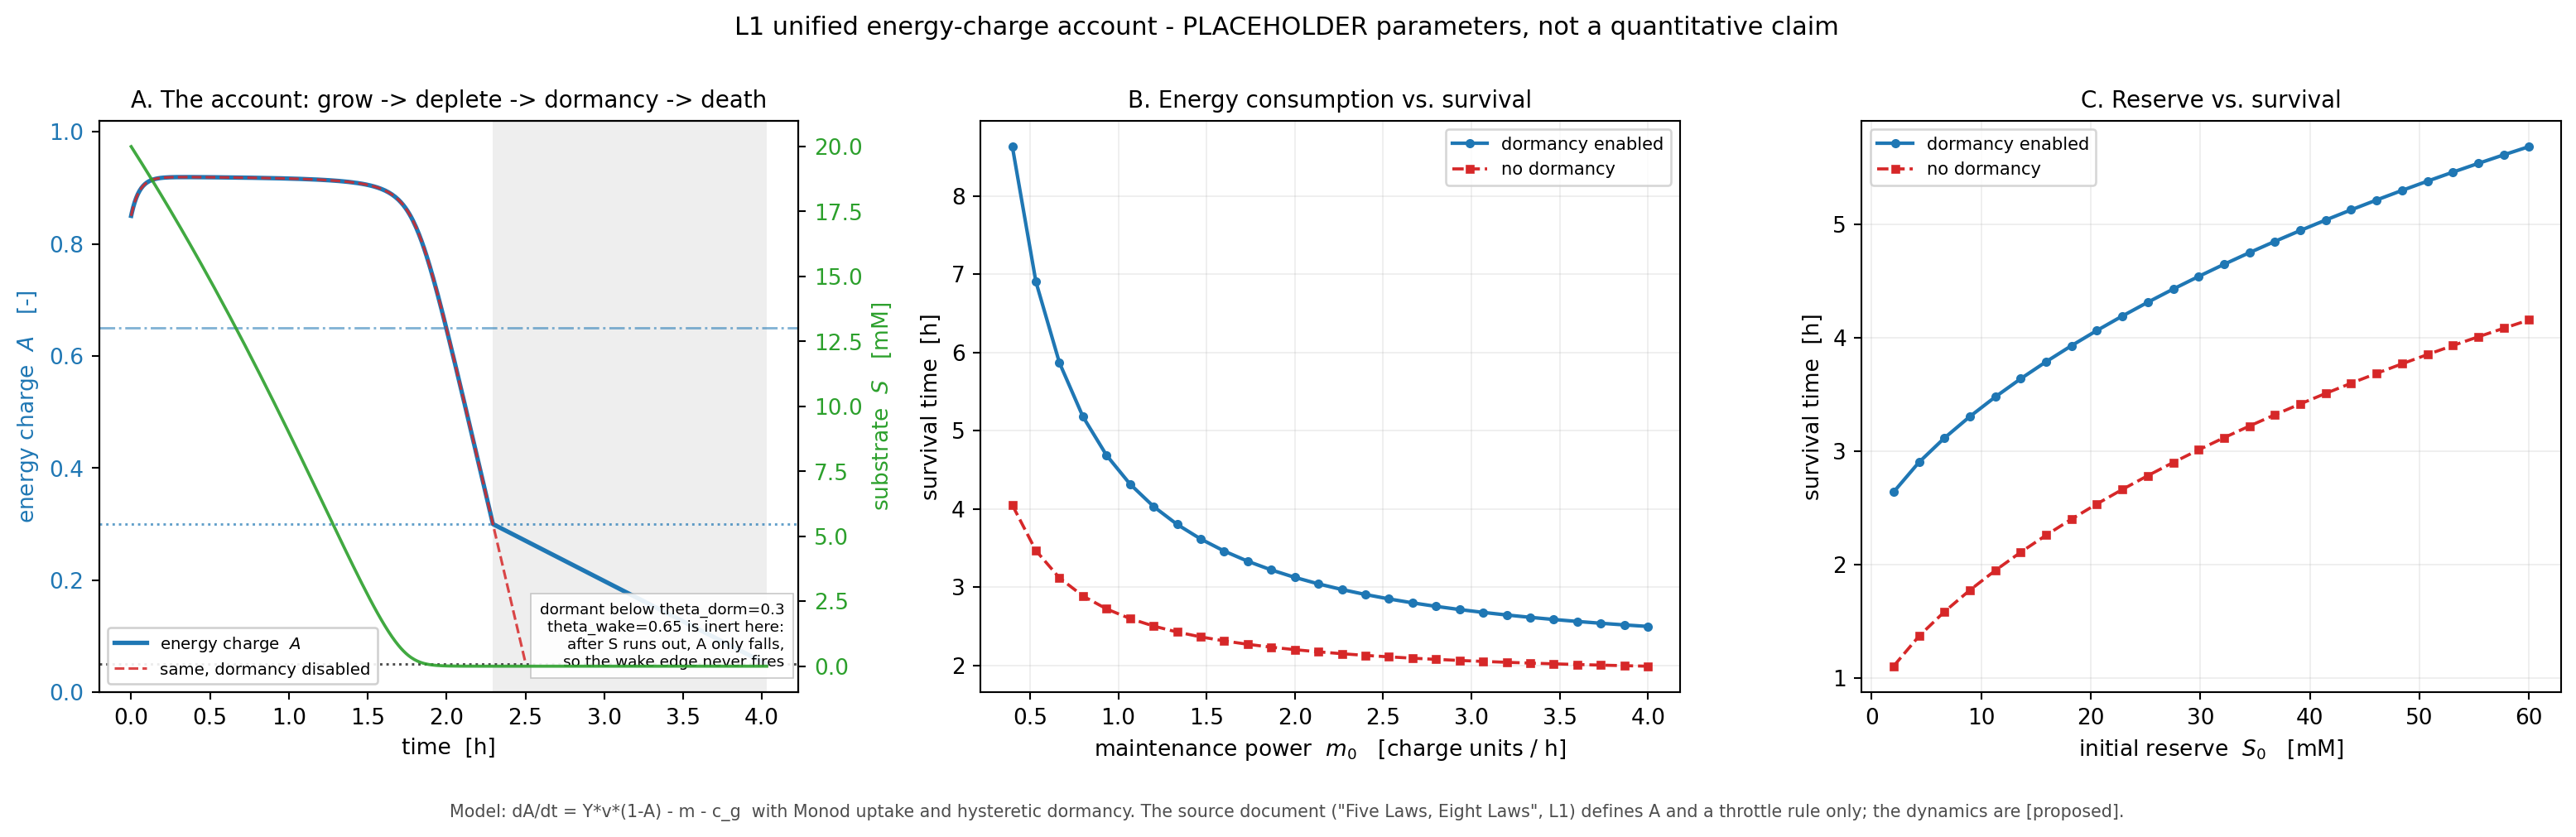
\includegraphics[width=1\linewidth,height=\textheight,keepaspectratio,alt={The L1 energy-charge account. (a) Growth, substrate depletion, dormancy and death, with dormancy enabled (solid) and disabled (dashed). (b) Survival against maintenance rate. (c) Survival against initial reserve. Open markers are censored, not death times.}]{figures/fig1_energy_account.png}
\caption{The L1 energy-charge account. (a) Growth, substrate depletion, dormancy and death, with dormancy enabled (solid) and disabled (dashed). (b) Survival against maintenance rate. (c) Survival against initial reserve. Open markers are censored, not death times.}
\end{figure}

\subsection{2.2 Axioms}\label{axioms}

The following nine statements are the entire starting set. Anything not derivable
from them is labelled empirical.

\textbf{Ax1 (uptake).} \(v(S)=V_{\max}S/(K_s+S+S^2/K_i)\), with
\(V_{\max}=10\), \(K_s=1\), \(K_i=4\). \(v\in C^\infty\), \(v(0)=0\), \(v\) is increasing on
\([0,\sqrt{K_sK_i})=(0,2)\) and decreasing beyond. The operating point is
\(S_0=0.5<2\), so \(C\) increases in \(R\) throughout the scenario. Figure 2 shows
the law and its inhibitory branch.

\begin{figure}
\centering
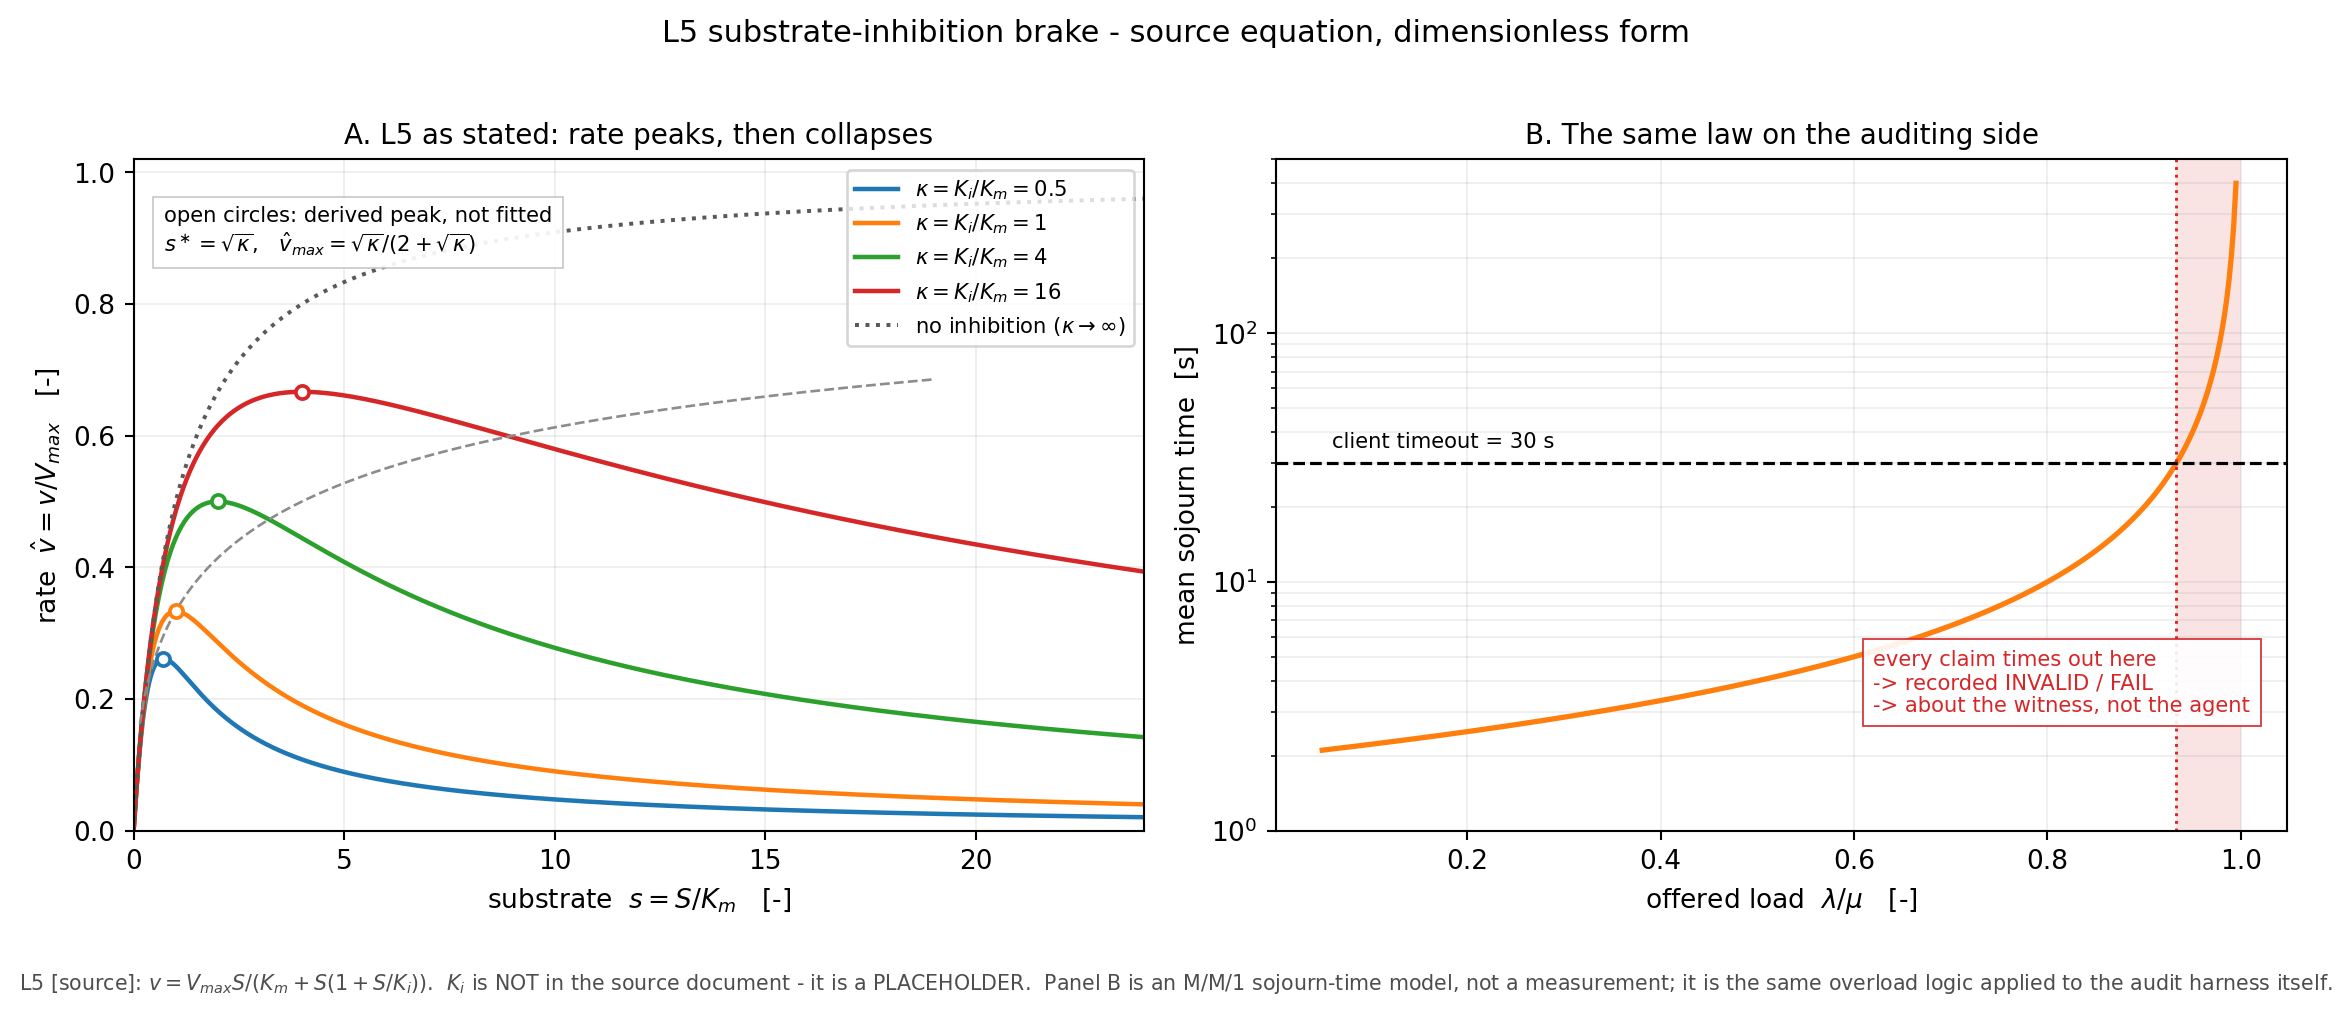
\includegraphics[width=1\linewidth,height=\textheight,keepaspectratio,alt={The uptake law and its inhibitory branch. (a) The rate rises to a derived maximum at the geometric mean of the half-saturation and inhibition constants, then collapses as the reciprocal of the substrate; open circles mark the analytic peak, the dashed curve the locus of achievable peaks. (b) The same overload logic on the auditing side: mean sojourn time in an M/M/1 queue.}]{figures/fig2_inhibition.png}
\caption{The uptake law and its inhibitory branch. (a) The rate rises to a derived maximum at the geometric mean of the half-saturation and inhibition constants, then collapses as the reciprocal of the substrate; open circles mark the analytic peak, the dashed curve the locus of achievable peaks. (b) The same overload logic on the auditing side: mean sojourn time in an M/M/1 queue.}
\end{figure}

\textbf{Ax2 (dormant charging, M1).} For \(m=\mathrm{dorm}\),
\(\dot A=Y\phi_v v(S)(1-A)-\phi_{\mathrm{dorm}}m_0\). This is the law on the
shock-free branch. During an episode the uptake is \(W=\sigma_sv(S)\), and the same
equation holds with \(v(S)\) replaced by \(W\); because D8 defines \(\chi\) on the peak
\(W\), the identity \(A_\infty=1-1/\chi\) is the fixed point of this equation exactly
when \(W=v(S)\), which is the branch on which Theorem 1's deadlock verdicts are
issued (I5).

\textbf{Ax3 (active accounting, M2).} For \(m=\mathrm{act}\),
\(\dot A=\dfrac{m_0}{D_0}[(1+\epsilon_m)d-c]\).

\textbf{Ax4 (delivery map).} \(d=c\cdot\mathbf{1}[C\ge c]\) for Type-A (atomic);
\(d=\min(c,C)\) for Type-B (divisible).

\textbf{Ax5 (commitment policy).} \(c_A\equiv D_0\); \(c_B=a\) with
\(a_{t+1}=\min(D_0,1.05a_t)\) on \texttt{PASS} and \(a_{t+1}=0.95a_t\) on \texttt{FAIL}.

\textbf{Ax6 (hysteresis switch; Type-B).} For an agent that may enter dormancy
(Type-B; I4 excludes Type-A), \(\mathrm{act}\to\mathrm{dorm}\) iff
\(A<\theta_{\mathrm{dorm}}\) or \(A_{\mathrm{sleep}}\) consecutive cycles were judged
\texttt{FAIL}; \(\mathrm{dorm}\to\mathrm{act}\) iff \(A\ge\theta_{\mathrm{wake}}\) for
\(\kappa\) consecutive cycles. The second entry condition is the verdict streak of
§2.7, not a load ratio; the implementation keeps it as \texttt{SLEEP\_AFTER=2}.

\textbf{Ax7 (environment).} \(R\) is multiplied by \(1-\varepsilon\) every \(10\) cycles,
so that \(R(t)=(1-\varepsilon)^{\lfloor t/P\rfloor}\);
\(\sigma=\sigma_s\) on cycles \(t\bmod P\in\{0,\dots,L-1\}\) and \(1\) otherwise.

\textbf{Ax8 (death).} \(A\le0\Rightarrow m=\mathrm{dead}\), irreversibly.

\textbf{Ax9 (independence).} Agents share the exogenous \(C(t)\) and do not interact.
\(v_i\) and \(m_{0,i}\) are independent static lognormal factors with
\(\sigma_v=0.08\), \(\sigma_m=0.12\).

\textbf{Inference rules.} Ten rules are used, and a statement derived with anything
else is not a proof in this paper: modus ponens (IR1); universal instantiation,
agent to population (IR2); induction, used for the cascaded product (IR3);
monotone convergence, used for \(A(t)\to A_\infty\) (IR4); comparison principle and
Gronwall, used for the quasi-static error (IR5); l'Hôpital and asymptotic
expansion, used for the tail of \(v\) (IR6); reductio, used for the no-loop theorem
and for the empty-set argument of §2.7 (IR7); Lyapunov functions, used for the
closed batch system (IR8); the law of large numbers, used for the \(N\to\infty\)
reading of the boundary (IR9); and the delta method, used for the interval on
\(\tau\) (IR10). A numerical agreement is not a proof, a parameter sweep is not a
proof, and a parameter chosen to produce a phenomenon is not a derivation: any
statement that rests on those three is recorded as an empirical regularity.

\textbf{Table 1. The eleven load-bearing assumptions of the audit, and what each supports.}

{\def\LTcaptype{none} % do not increment counter
\begin{longtable}[]{@{}
  >{\raggedright\arraybackslash}p{(\linewidth - 6\tabcolsep) * \real{0.0952}}
  >{\raggedright\arraybackslash}p{(\linewidth - 6\tabcolsep) * \real{0.2976}}
  >{\raggedright\arraybackslash}p{(\linewidth - 6\tabcolsep) * \real{0.2738}}
  >{\raggedright\arraybackslash}p{(\linewidth - 6\tabcolsep) * \real{0.3333}}@{}}
\toprule\noalign{}
\begin{minipage}[b]{\linewidth}\raggedright
ID
\end{minipage} & \begin{minipage}[b]{\linewidth}\raggedright
assumption in words
\end{minipage} & \begin{minipage}[b]{\linewidth}\raggedright
axiom / decision that realises it
\end{minipage} & \begin{minipage}[b]{\linewidth}\raggedright
result that fails if it is false
\end{minipage} \\
\midrule\noalign{}
\endhead
\bottomrule\noalign{}
\endlastfoot
A1 & uptake is algebraic, not stateful & Ax1 & \(\chi\) undefined; Theorem 1 not computable \\
A5 & the active phase is linear with no feedback & Ax3 (M2) & recovery to \(A\approx0.95\); no extinction \\
A7 & M1 and M2 may be joined at the switch & Ax6 & two theorems about two systems; the join is unjustified \\
A8 & failed work earns nothing & Ax3 with \(d=0\) & extinction disappears \\
A10 & Type-A tasks are atomic & Ax4 & positive margin at cycle 100; no step \\
A13 & no reproduction, inheritance or variation & Ax9 & cohort survival, not evolution \\
A14 & agents are independent & Ax9 & frequency dependence; a genuine phase transition possible \\
A16 & utilisation is fixed & scenario choice & ordering reverses near \(U=0.445\) \\
A20 & the wake gate is peak-to-peak & wake rule, §2.7 & \(279\to233\) or \(983\) \\
A21 & deadlock needs three shock-free samples & §2.7, I5 & spurious left tail at \(\theta=0.90\) \\
A27 & all eleven kinetic constants are placeholders & parameter table & numbers are dimensionless shapes, not predictions \\
\end{longtable}
}

\subsection{2.3 Definitions}\label{definitions}

Twelve definitions are used. They are numbered to agree with the formal
verification report, so that a reader can move between the two documents without
re-indexing.

\textbf{D1 (delivery and commitment).} \(d_i(t)\) is the work that actually landed in
cycle \(t\); \(c_i(t)\) is the scope the agent committed to before the cycle began.

\textbf{D2 (availability).} \(\mathrm{Avail}_i(t)=d_i(t)/c_i(t)\) for \(c_i(t)>0\), with
the convention \(0/0=0\). This makes
\(\mathrm{Obs}_i=\mathrm{Cap}_i\cdot\mathrm{Avail}_i\) an identity rather than a
theorem, which is why availability cannot be used as independent evidence about
capacity.

\textbf{D3 (observation).} \(\mathrm{Obs}_i(t)=\mathrm{Cap}_i(t)\cdot\mathrm{Avail}_i(t)\).
Type-A records \(\mathrm{Cap}_i=c_i\), so its observation is the claim; Type-B
records \(\mathrm{Cap}_i=d_i\), so its observation is the delivery.

\textbf{D4 (deadlock).} \(\mathrm{DL}_i:\iff m_i=\mathrm{dorm}\ \land\
\lim_{t\to\infty}A_i(t)<\theta_{\mathrm{wake}}\ \land\ \exists S>0:v(S)>0\).
The third clause separates deadlock (resources present, charge unreachable) from
starvation (resources absent).

\textbf{D5 (stranding).} \(\mathrm{ST}_i:\iff m_i=\mathrm{dorm}\ \land\
\forall t\ge t_0:W_i(t)<w_h\), \(w_h=0.85\,W_i(1)\). \(\mathrm{DL}\) is a statement
about the limit of \(A\); \(\mathrm{ST}\) is a statement about the supply side. Neither
implies the other.

\textbf{D6 (extinction).} \(E_A(t):\iff\#\{i:\ \mathrm{kind}_i=A,\ m_i\ne
\mathrm{dead}\}=0\).

\textbf{D7 (collapse).} Operational definition used by the code: with \(b\) the median
of \(d_A\) over the first 20 cycles,
\(t_{\mathrm{collapse}}=\max\{t:d_A(t)\ge b/2\}+1\). This is a definition, not a
theorem; a different threshold gives a different cycle.

\textbf{D8 (charging margin).} \(\chi_i(t)=Y\phi_vW_i(t)/(m_0\phi_{\mathrm{dorm}})\) and
\(\theta^\ast_i(t)=1-1/\chi_i(t)\). With the \(V_{\max}\) normalisation
\(\chi_{0,i}=Y\phi_vV_{\max}/(m_0\phi_{\mathrm{dorm}})\) and \(f_i=W_i/V_{\max}\),
one has \(\chi_i=f_i\chi_{0,i}\).

\textbf{D9 (cumulative causal potential).}
\(\Phi_n=S_0-\hat S_n=\sum_{k\le n}(\hat S_{k-1}-\hat S_k)\).

\textbf{D10 (hysteresis loop).} A state sequence that returns repeatedly to
\([\theta_{\mathrm{dorm}},\theta_{\mathrm{wake}}]\) with the upward and downward
edges triggered by conditions of different type (one autonomous, one exogenous).
We flag here that this definition writes \emph{asymmetry} into the definiens, so that
``asymmetry is necessary for a loop'' is a tautology under D10 and false under the
standard dynamical-systems reading; §2.8 uses the standard reading, which is why
the general claim is withdrawn.

\textbf{D11 (phase transition).} An order parameter \(s(g)\) is non-analytic at some
\(g_c\), or the susceptibility \(\chi=-\partial s/\partial g\) diverges there, and the
behaviour survives \(N\to\infty\). This is the strict definition used to reject the
phase-transition reading in §3.5.

\textbf{D12 (functional).} Alive and not stranded: \(m\ne\mathrm{dead}\ \land\
\lnot\mathrm{ST}\). This is the ordinate of panel 1 of the sandbox figure in §3.1.

\subsection{2.4 The two-regime model}\label{the-two-regime-model}

Figure 3 shows the phenomenon the switch \texttt{Ax6} is there to represent: in a
periodic feeding regime the charge returns to the band every cycle while the
substrate does not, so the loop lives in \(A\) and not in \(S\). Figure 4 shows the
same structure in a closed fed batch, where the cycle is a genuine limit cycle
and the deadlock at \(\theta_{\mathrm{wake}}=0.99\) is visible as an agent pinned
below the threshold with substrate still in the vessel.

\begin{figure}
\centering
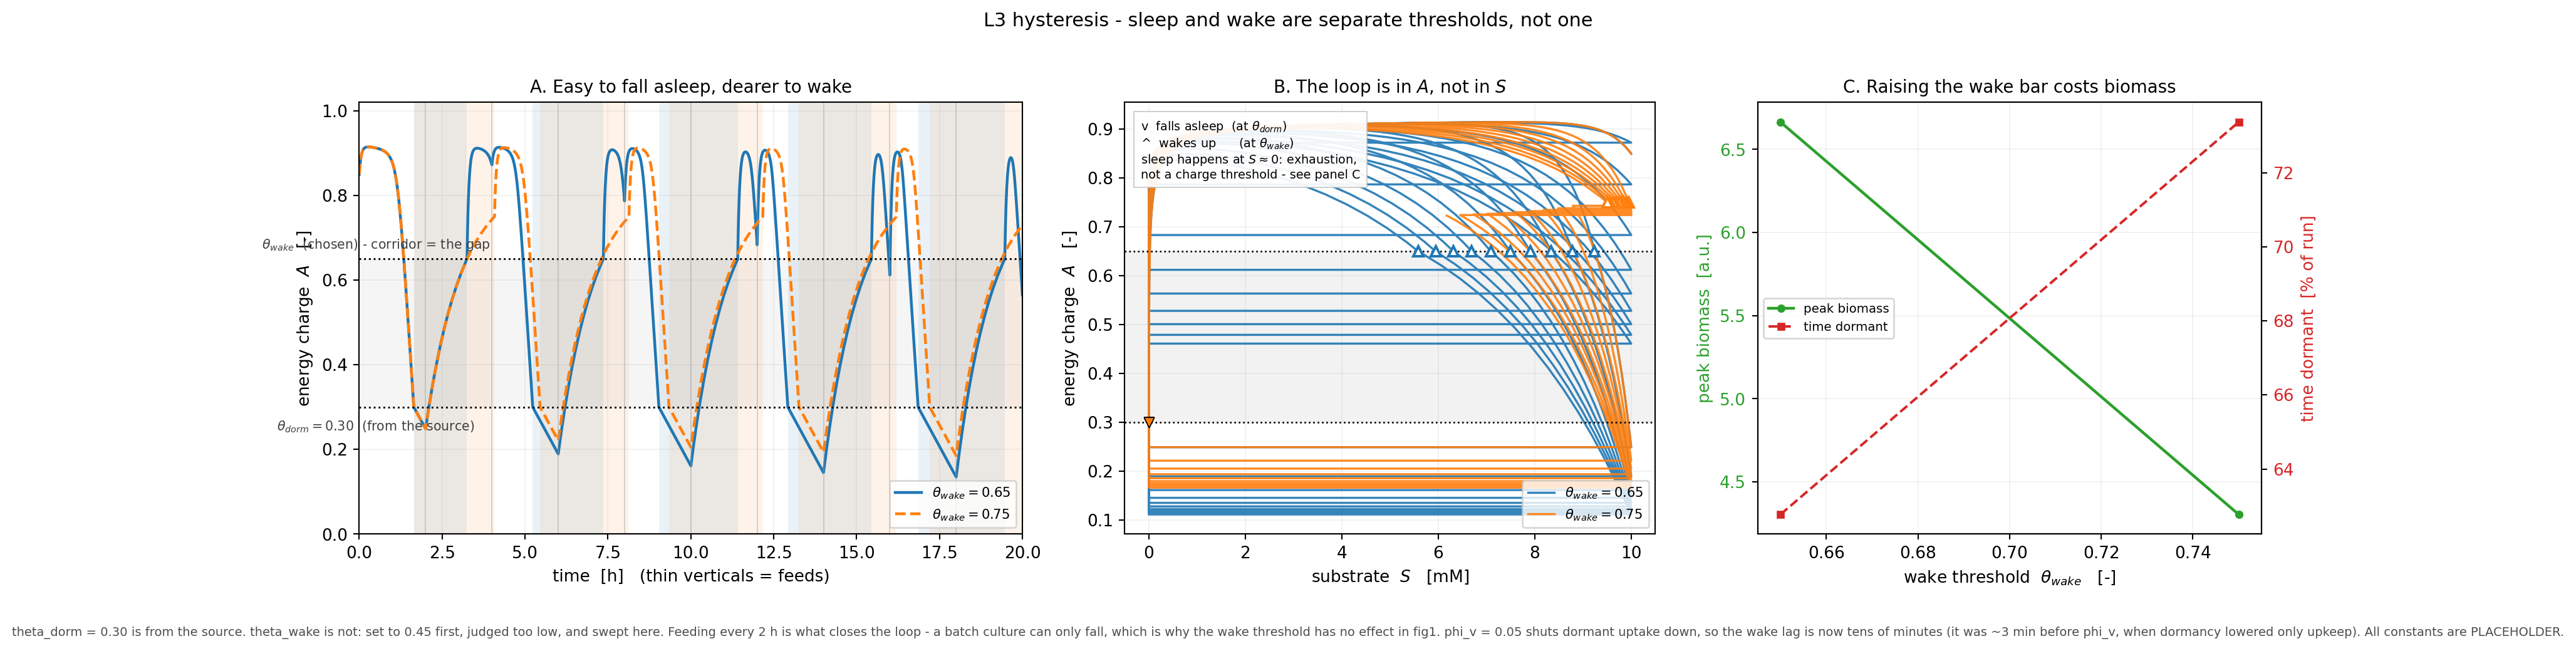
\includegraphics[width=1\linewidth,height=\textheight,keepaspectratio,alt={Hysteresis in a 2 h feeding regime. (a) Charge over time. (b) The (S,A) plane: the loop lives in A while S returns to zero every cycle. (c) Peak biomass against the wake threshold.}]{figures/fig3_hysteresis_loop.png}
\caption{Hysteresis in a 2 h feeding regime. (a) Charge over time. (b) The \((S,A)\) plane: the loop lives in \(A\) while \(S\) returns to zero every cycle. (c) Peak biomass against the wake threshold.}
\end{figure}

\begin{figure}
\centering
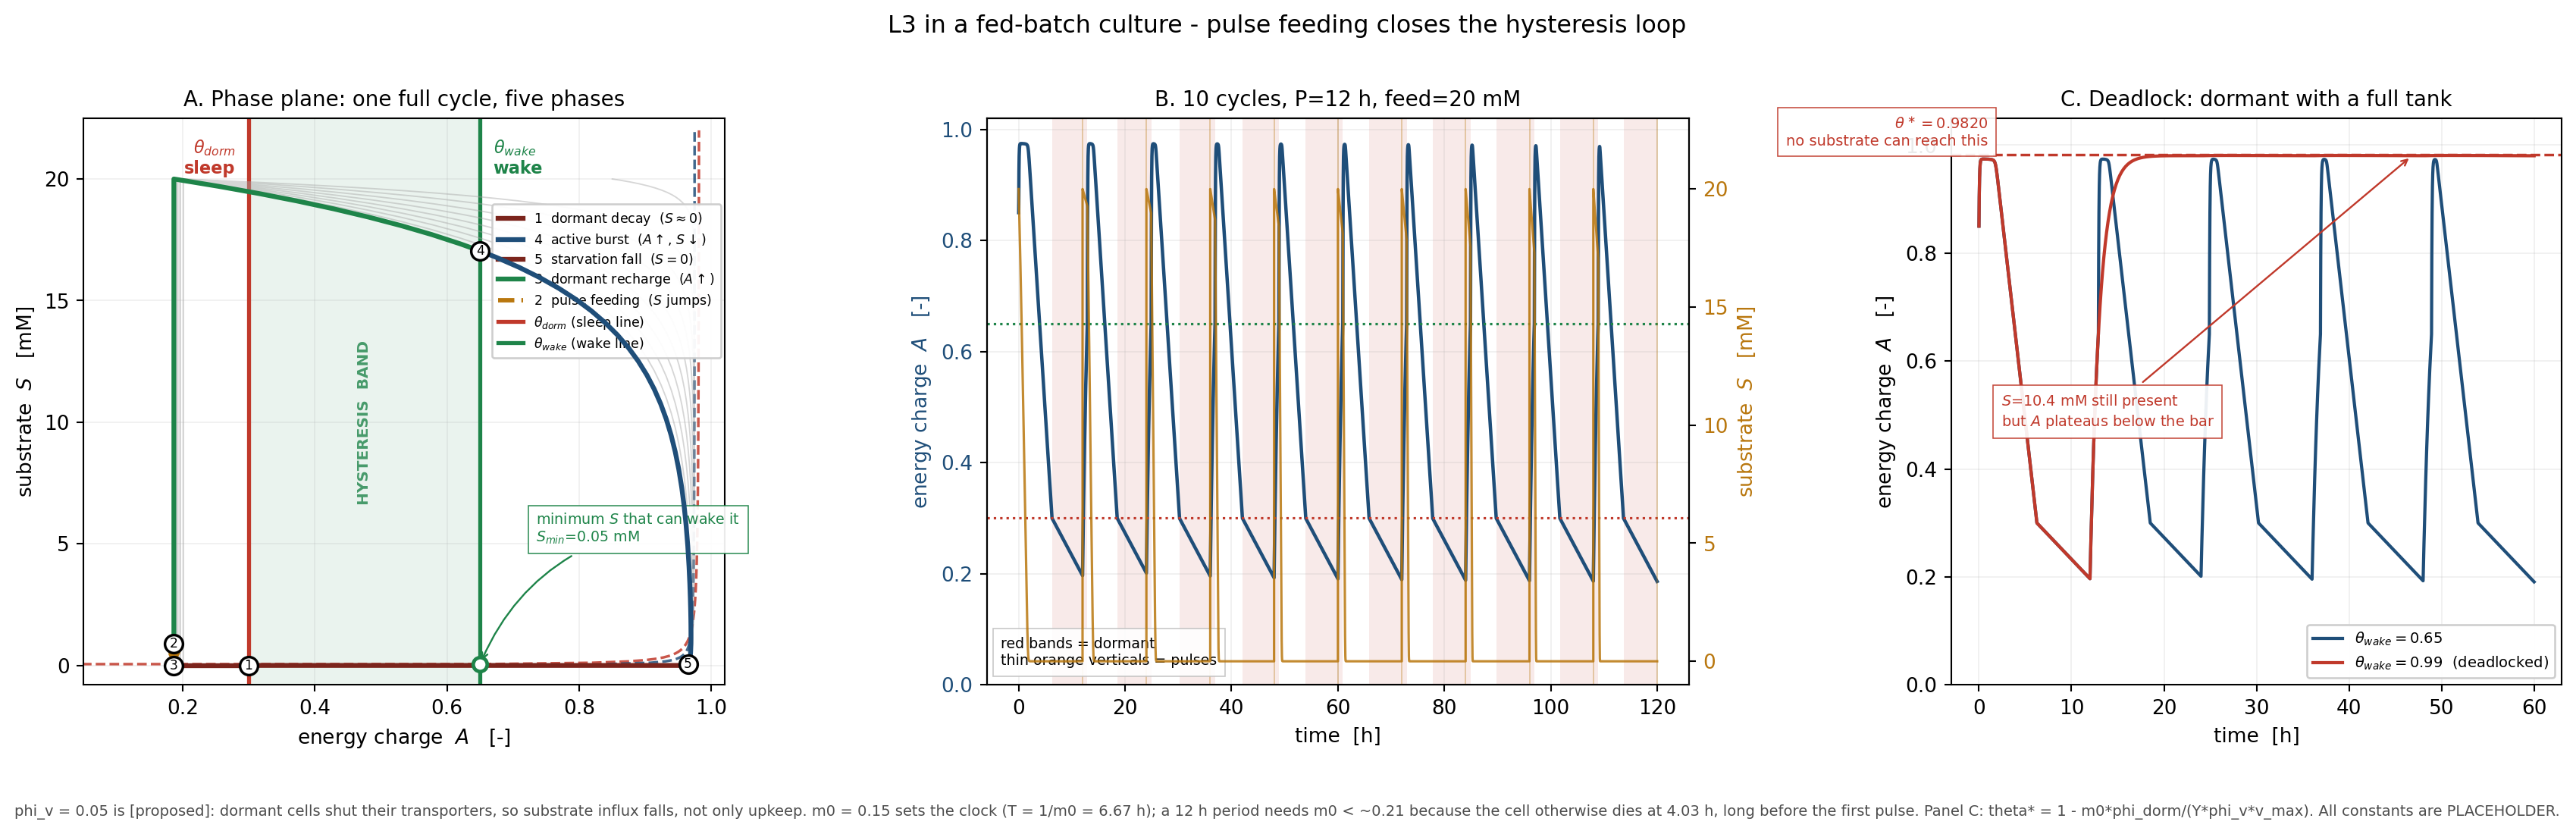
\includegraphics[width=1\linewidth,height=\textheight,keepaspectratio,alt={Fed batch: a closed five-phase limit cycle. (a) Phase plane with one cycle highlighted. (b) Time series with dormant bands and pulses. (c) Deadlock at a wake threshold of 0.99: the agent is pinned below the bar with substrate still available.}]{figures/fig4_fed_batch_hysteresis.png}
\caption{Fed batch: a closed five-phase limit cycle. (a) Phase plane with one cycle highlighted. (b) Time series with dormant bands and pulses. (c) Deadlock at a wake threshold of 0.99: the agent is pinned below the bar with substrate still available.}
\end{figure}

\textbf{Proposition 1 (M1 and M2 are not equivalent).} Fix \(v>0\) and write
\(a=Y\phi_vv>0\), \(b=\phi_{\mathrm{dorm}}m_0>0\). \texttt{M1} has the interior fixed point
\(A^\ast_{\mathrm{M1}}=1-b/a=1-\phi_{\mathrm{dorm}}m_0/(Y\phi_vv)\), which is
exponentially stable with rate \(a=Y\phi_vv\). \texttt{M2} with \(d=0\) has no interior
fixed point and decreases at the constant rate \(m_0c/D_0\); with \(d=c\) it
increases without bound until the projection acts. The two have opposite
qualitative behaviour for every \(v>0\).

The fixed point is the same expression as \(A_\infty=1-1/\chi\) of Lemma 1, because
D8 defines \(\chi=Y\phi_vv/(\phi_{\mathrm{dorm}}m_0)=a/b\); a reader who meets
\(1-1/\chi\) in §2.5 and \(1-b/a\) here is reading one formula, not two.

\emph{Proof.} \(\partial\dot A/\partial A=-Y\phi_vv=-a<0\) for \texttt{M1}, so the deviation
from the fixed point decays as \(e^{-at}\); \(\partial\dot A/\partial A=0\) for \texttt{M2},
which is therefore affine in \(A\) and has no interior fixed point when \(d=0\).
\(\square\)

\textbf{Corollary 1 (the 107-cycle extinction belongs to M2).} On the reference
capacity trajectory \texttt{M1} predicts
\(A^\ast=1-\phi_{\mathrm{dorm}}m_0/(Y\phi_vv)=1-0.018/0.32=0.94375\) at the day-1
peak \(W(1)=v(S_0)=3.2\), and \(0.9402\) at \(W(100)=3.008\), both above \(A(0)=0.85\);
hence \(A\) would rise toward the fixed point with \(\tau=3.125\) cycles and would
not fall. The largest shock in the record subtracts at most \(Lm_0=0.30\), about a
third of the fixed point, and even at the largest sampled \(m_{0,i}=0.183\) the
subtraction is \(2m_{0,i}=0.37\): \(A\) stays above \(\theta_{\mathrm{dorm}}=0.30\), so
no shock drives it into dormancy, and the loss is restored within
\(3\tau\approx9\) cycles. The onset at cycle 100 lies seven cycles after the
episode 92--93 and fifteen before the next, so no shock is inside the decisive
window. \texttt{M2} with \(d=0\) decreases at \(m_0\) per cycle and crosses zero in
\(A(100)/m_0\approx4.6\) cycles. The extinction is a property of the accounting
law, not of the metabolic law.

This proposition is the reason the paper does not present a unified equation.
\texttt{Ax6} joins the two regimes; the join is assumption A7, and it is an assumption
because no limit of one law produces the other at the switching manifold: M1 has
a stable interior point where M2 has none, and M2 has a conserved linear drift
where M1 has exponential relaxation.

\subsection{2.5 Theorem 1: the deadlock boundary}\label{theorem-1-the-deadlock-boundary}

Figure 1 gives the charge account that Lemma 1 formalises: growth, substrate
depletion, dormancy and death for the same strain with dormancy enabled and
disabled, together with survival against maintenance rate and against initial
reserve. Figure 5 is the phase diagram of the resulting boundary in the
\((\theta_{\mathrm{wake}},\chi)\) plane, with the analytic line of Theorem 1 drawn
on it.

\begin{figure}
\centering
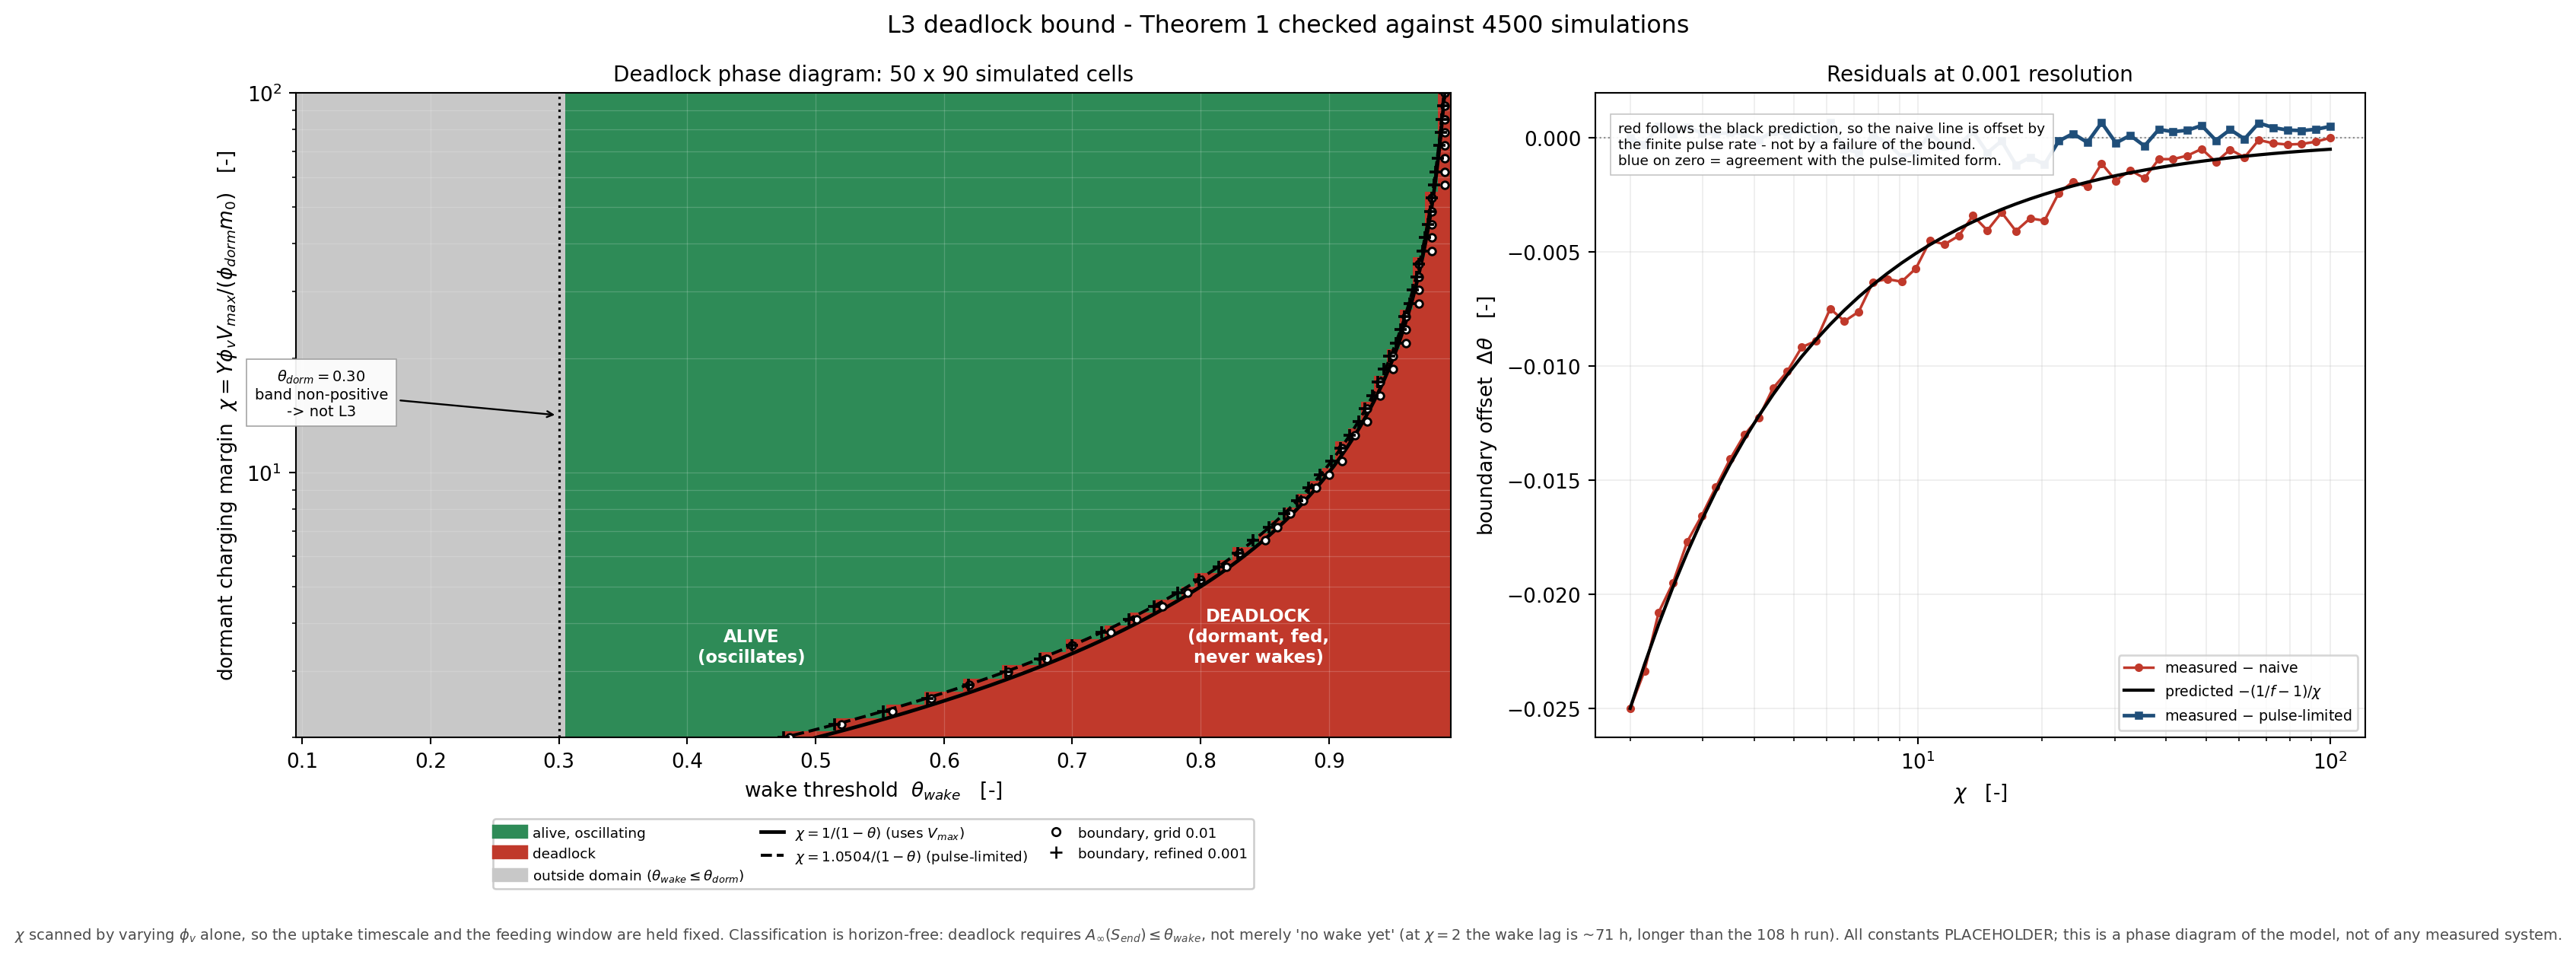
\includegraphics[width=1\linewidth,height=\textheight,keepaspectratio,alt={The deadlock phase diagram over the wake threshold and the charging margin (4500 cells). The black line is Theorem 1 in its maximum-rate form, the dashed line the pulse-corrected form. Right panel: boundary offsets against the margin, showing the measured deviation tracking the predicted offset rather than sitting on zero.}]{figures/fig5_deadlock_phase_diagram.png}
\caption{The deadlock phase diagram over the wake threshold and the charging margin (4500 cells). The black line is Theorem 1 in its maximum-rate form, the dashed line the pulse-corrected form. Right panel: boundary offsets against the margin, showing the measured deviation tracking the predicted offset rather than sitting on zero.}
\end{figure}

\textbf{Lemma 1 (closed form).} If \(S\) is fixed on the charging time scale, \texttt{M1} has

\[
A(t)=A_\infty+\big(A(0)-A_\infty\big)e^{-t/\tau},\qquad
A_\infty=1-\frac{1}{\chi},\qquad
\tau=\frac{1}{m_0\phi_{\mathrm{dorm}}\chi}.
\]

\emph{Proof.} Write \texttt{Ax2} as \(\dot A=-(A-A_\infty)/\tau\) and integrate. \(\square\)

\textbf{Lemma 2 (monotonicity).} \(A(t)\) is monotone between \(A(0)\) and \(A_\infty\) and
does not oscillate. \emph{Proof.} The error term is an exponential with a fixed sign. \(\square\)

\textbf{Lemma 3 (no crossing).} If \(A(0)\le\theta\) and \(A_\infty<\theta\), then
\(A(t)<\theta\) for all \(t>0\). \emph{Proof.} By Lemma 2, \(A(t)\) lies between \(A(0)\) and
\(A_\infty\); if \(A(0)=\theta\) the approach is strict. \(\square\)

\textbf{Lemma 4 (threshold equivalence).} For \(\theta\in(0,1)\) and \(\chi=f\chi_0\),

\[
A_\infty<\theta\iff\chi<\frac{1}{1-\theta}\iff\chi_0<\frac{1}{f(1-\theta)}.
\]

\emph{Proof.} \(1-1/\chi<\theta\iff\chi<1/(1-\theta)\); substitute \(\chi=f\chi_0\). \(\square\)

\textbf{Theorem 1.} Assume

\begin{itemize}
\tightlist
\item
  \textbf{H1 (entry):} at the first dormant cycle, \(A(0)\le\theta_{\mathrm{wake}}\);
\item
  \textbf{H2 (quasi-static):} \(S\) is constant to within the tolerance of Lemma 1 on
  the scale \(\tau\);
\item
  \textbf{H3 (wake rule):} waking requires \(A\ge\theta_{\mathrm{wake}}\) for \(\kappa\)
  consecutive cycles.
\end{itemize}

Then

\[
\mathrm{DL}\iff A_\infty<\theta_{\mathrm{wake}}
\iff \chi<\frac{1}{1-\theta_{\mathrm{wake}}}=:\chi_{\min}
\iff \chi_0<\frac{1}{f\,(1-\theta_{\mathrm{wake}})}=\frac{\chi_{\min}}{f}.
\]

\emph{Proof.} (\(\Leftarrow\)) By H1 and Lemma 3, \(A(t)<\theta_{\mathrm{wake}}\) for all
\(t\ge0\), so H3 never fires; by D4, deadlock. (\(\Rightarrow\)) Suppose
\(A_\infty>\theta_{\mathrm{wake}}\). By Lemma 2, \(A\) approaches \(A_\infty\) from
below. If \(A(0)\le\theta_{\mathrm{wake}}\), there is a finite

\[
t_c=\tau\ln\frac{A_\infty-A(0)}{A_\infty-\theta_{\mathrm{wake}}}
\]

with \(A(t_c)=\theta_{\mathrm{wake}}\); after \(\kappa\) further cycles H3 is
satisfied. If \(A(0)>\theta_{\mathrm{wake}}\) the threshold is met immediately.
Hence no deadlock. Lemma 4 gives the equivalence chain. \(\square\)

\textbf{The critical case is a definition gap, not a theorem.} At
\(\chi=\chi_{\min}\) we have \(A_\infty=\theta_{\mathrm{wake}}\); \(A\) approaches
the threshold strictly from below and never attains it, so H3 never fires while
D4 (strict inequality) does not classify the agent as deadlocked. The interval
\(\chi=\chi_{\min}\) is therefore a measure-zero set on which the agent is
functionally dead and formally not deadlocked. Both the theorem and the code use
the strict reading.

\textbf{Corollary 2 (the boundary has a horizon).} Because \(\chi\) is a function of the
current peak,

\[
\theta^\ast(t)=1-\frac{1}{\chi(t)}=1-\frac{1}{c_0W(t)},
\qquad c_0=\frac{Y\phi_v}{m_0\phi_{\mathrm{dorm}}}.
\]

Under geometric drift \(W\) decreases, so \(\theta^\ast\) decreases. A threshold
quoted without its horizon is the boundary of a stopping rule, not of the system.
Numerically, \(\theta^\ast(1)=0.9437\) and \(\theta^\ast(300)=0.9317\).

\textbf{Corollary 3 (marginal capacity).} With \(\chi=c_0W\),

\[
\frac{\partial A_\infty}{\partial W}=\frac{1}{c_0W^2}=\frac{1}{\chi W}>0,
\qquad \frac{\partial A_\infty}{\partial W}\to0\ \ (W\to\infty).
\]

Inside the deadlock region, restoring \(A_\infty>\theta_{\mathrm{wake}}\) requires
the finite relative increment \(\Delta W/W=\chi_{\min}/\chi-1>0\). An infinitesimal
increase changes no verdict. The statement is local and it is about \(W\) as a free
variable; \(W\) is not free, and the next corollary is what that costs.

\textbf{Corollary 3\('\) (the uptake peak caps the boundary).} With \(W(R)=v(S_0R)\sigma\),
\(\sigma\le1\), and (Ax1),

\[
\chi(R)=\chi_0\,\frac{v(S_0R)}{V_{\max}}\,\sigma
\ \le\ \chi_0\,\frac{v_{\max}}{V_{\max}}
=\frac{\chi_0}{1+2\sqrt{K_s/K_i}}\ =:\ \chi_{\max},
\]

with equality iff \(S_0R=\sqrt{K_sK_i}\) and \(\sigma=1\). Consequently

\[
\sup_{R>0}A_\infty(R)=1-\frac{1}{\chi_{\max}}=0.964,
\qquad
\sup_{R>0}\theta^\ast(R)=1-\frac{1+2\sqrt{K_s/K_i}}{\chi_0}=0.964 .
\]

\emph{Proof.} Differentiating (Ax1),
\(v'(S)=V_{\max}(K_s-S^2/K_i)\big/(K_s+S+S^2/K_i)^2\), which vanishes exactly at
\(S=\sqrt{K_sK_i}\) and changes sign there; at that point
\(v_{\max}=V_{\max}/(1+2\sqrt{K_s/K_i})\). Substituting \(\chi=c_0W\) with
\(\chi_0=c_0V_{\max}\) gives \(\chi_{\max}\), and Lemma 4 gives the boundary.
\(\square\)

Three consequences, and the third is a retraction. First, above \(\theta=0.964\) no
substrate level can restore an agent: the ceiling is below the bar, and past the
peak more substrate \emph{lowers} \(\chi\). This is the regime of the \(\theta=0.99\)
example. Second, below \(0.964\) a flood does help, and it rescues exactly the agents
with \(\chi(t)>\chi_{\min}v(S_0)/v_{\max}=11.37\); in the reference scenario
\(\chi(t)\in[14.63,17.78]\), so every deadlocked agent qualifies. Third: the claim
that adding resources cannot exit a deadlock is therefore false in the range this
paper's sweep covers, and we withdraw it in that range. What the inhibition term
rules out is not escape but \emph{unbounded} escape --- and that is the difference between
the slogan we published and the theorem we can prove.

\textbf{Remark on H1.} H1 is not a technicality. If dormancy is entered through the
verdict clause (two consecutive \texttt{FAIL} cycles) rather than through low charge,
then \(A(0)\) can exceed
\(\theta_{\mathrm{wake}}\) while \(A_\infty<\theta_{\mathrm{wake}}\). Take
\(A(0)=0.9\), \(\theta_{\mathrm{wake}}=0.65\), \(A_\infty=0.5\): the crossing time is
\(t_c=\tau\ln(0.4/0.15)=0.98\tau\), so for \(\kappa\le0.98\tau\) the agent wakes
before it falls below the threshold and is not deadlocked. A verdict issued on
the first dormant cycle is therefore unsound. The implementation this paper
supersedes did exactly that; §2.7, invariant I5, states the replacement.

\subsection{2.6 The atomic mechanism}\label{the-atomic-mechanism}

Theorem 1 concerns the dormant phase. The extinction in the base scenario occurs
in the active phase, and its mechanism is separate and purely algebraic.

\textbf{Proposition 2 (delivery onset).} Let \(\rho(t)=C(t)/C_0\) and let the Type-A
claim be \(c_i=U C_{0,i}\), so that \(c_i/C_i(t)=U/\rho(t)\) for every agent \(i\).
Then \(d_i(t)=c_i\) iff \(\rho(t)\ge U\), and \(d_i(t)=0\) otherwise. Hence the first
cycle with \(d_i=0\) is \(\min\{t:\rho(t)<U\}\), independent of \(i\) and of \(v_i\).

\emph{Proof.} Immediate from \texttt{Ax4} and the proportionality of claim and capacity to
\(v_i\). \(\square\)

\textbf{Proposition 3 (drought rate).} The implemented form of \texttt{Ax3} is
\(\Delta A_i=m_{0,i}\big[(1+\epsilon_m)d_i-c_i\big]/D_{0,i}\), i.e.~the prefactor is
the per-agent upkeep rate \(m_{0,i}\) itself. While \(d_i=0\) and \(c_i=D_{0,i}\) this gives
\(\Delta A_i=-m_{0,i}\) exactly. Hence the time from onset to death is
\(A_i(t_c)/m_{0,i}\) and the death cycle is \(t_c+\lceil A_i(t_c)/m_{0,i}\rceil\).

\emph{Proof.} Substitute \(d=0\), \(c=D_0\) in \texttt{Ax3}. \(\square\)

Propositions 2 and 3 give the two observables of the base run. With \(U=0.93\) and
\(\rho(99)=0.9342\), \(\rho(100)=0.9271\), the onset is exactly cycle 100, and no
agent dies on that cycle because \(A_i(100)>0\). With \(A_i(100)\in[0.6158,0.7558]\)
and \(m_{0,i}\in[0.1162,0.1829]\), the deaths fall in cycles \(104\)--\(107\), four to
seven cycles after the onset, entirely inside a shock-free interval (the nearest
shocks are at 92--93 and 115--116). The spread is not noise: it is the heterogeneity
of \(m_{0,i}\), which is the only parameter that differs across Type-A agents in this
equation.

\textbf{Corollary 4 (drought clock).} Suppose that at some cycle \(t_s\) every Type-A
agent is at the projection \(A=1\), and let

\[
\delta=\sum_{s=t_s+1}^{t_c}\Big(1-\epsilon_m\,\mathbf{1}[\text{PASS at }s]\Big)
\]

be the deficit accumulated between \(t_s\) and the onset, measured in units of
\(m_{0,i}\). Then \(A_i(t_c)=1-\delta m_{0,i}\) and

\[
t_{\mathrm{death},i}=t_c+\left\lceil \frac{1}{m_{0,i}}-\delta \right\rceil .
\]

\emph{Proof.} Each cycle adds \(+\epsilon_m m_{0,i}\) on \texttt{PASS} and \(-m_{0,i}\) otherwise,
and the projection is inactive after \(t_s\) by hypothesis. Sum and divide by
\(m_{0,i}\). \(\square\)

In the base run the last cycle at which every Type-A agent is at the projection is
91; the deficit to cycle 100 is \(\delta=3-0.15\times6=2.1\), so
\(A_i(100)=1-2.1\,m_{0,i}\) exactly. The deaths predicted by the corollary are
distributed over cycles 104--107 with multiplicities \(11,23,13,3\), which is the
observed distribution. The four-cycle spread of the extinction is therefore a
deterministic function of the \(m_{0,i}\) sample, not a stochastic effect.

The quantity the corollary makes available to an operator is the interval between
the saturation reference and the death,
\(t_{\mathrm{death}}-t_c=\lceil 1/m_{0,i}-\delta\rceil\in[4,7]\) cycles. It is worth
separating this from the raw headroom \(1/m_{0,i}\in[5.47,8.61]\): the offset between
them is the deficit \(\delta=2.1\), already spent before the clock starts, and only
the reduced interval is a lead time that can be promised to anyone.

\textbf{Assumption A28 (pre-shock saturation).} Every Type-A agent attains \(A=1\) under
the projection before the first shock cycle.

Corollary 4 takes the saturation reference at \(t_s=91\) and treats \(\delta\) as a
constant; that step presumes the agents saturated before the first shock, which is
not implied by the axioms. The presumption is stated here rather than in passing,
and it is verified rather than assumed: on the \texttt{PASS} branch,
\(\Delta A_i=\epsilon_m m_{0,i}\), so
\(t_{\mathrm{sat},i}=\lceil(1-A_0)/(\epsilon_m m_{0,i})\rceil=\lceil1/m_{0,i}\rceil
\in[6,9]\) for \(m_{0,i}\in[0.1162,0.1829]\), against a first shock at cycle 23. The
margin is 14 cycles. A28 is recorded as an appended assumption and is \emph{not} added
to the eleven load-bearing entries of Table 1, because no theorem fails when it
fails: only the closed-form multiplicities of Corollary 4 degrade to a numerical
observation. Appendix A.28 gives the proof and the parameter range over which it
survives.

\textbf{The break-even comparison.} Flow break-even requires
\(\rho\ge U/(1+\epsilon_m)=0.93/1.15=0.8087\), whereas delivery requires
\(\rho\ge U=0.93\). At the onset \(\rho=0.9271\), which is above break-even. Had
partial delivery been admissible, the net flow would have been
\(1.15\times0.9271-0.93=+0.1362\), i.e.~positive. The extinction is therefore not
insolvency; it is the discontinuity introduced by atomicity (assumption A10),
acting on a system that is still in flow surplus.

\subsection{2.7 The R7 mechanism}\label{the-r7-mechanism}

\textbf{Semantics.} The four values are defined by the relation between claim and the
part of the scope that exists:

{\def\LTcaptype{none} % do not increment counter
\begin{longtable}[]{@{}
  >{\raggedright\arraybackslash}p{(\linewidth - 4\tabcolsep) * \real{0.3333}}
  >{\raggedright\arraybackslash}p{(\linewidth - 4\tabcolsep) * \real{0.3333}}
  >{\raggedright\arraybackslash}p{(\linewidth - 4\tabcolsep) * \real{0.3333}}@{}}
\toprule\noalign{}
\begin{minipage}[b]{\linewidth}\raggedright
verdict
\end{minipage} & \begin{minipage}[b]{\linewidth}\raggedright
condition
\end{minipage} & \begin{minipage}[b]{\linewidth}\raggedright
meaning
\end{minipage} \\
\midrule\noalign{}
\endhead
\bottomrule\noalign{}
\endlastfoot
\texttt{PASS} & \(d=c>0\) & the claimed scope existed and was delivered \\
\texttt{FAIL} & \(c>0,\ C=0\) & the claimed scope was attempted; nothing of it exists \\
\texttt{INVALID} & \(c>0,\ 0<C<c\), or a confirmed deadlock (capacity may be sufficient) & the claimed scope was attempted; part of it does not exist \\
\texttt{NOT\_RUN} & \(c=0\) or \(m=\mathrm{dorm}\) or \(m=\mathrm{dead}\) & no attempt \\
\end{longtable}
}

\texttt{FAIL} and \texttt{INVALID} are not degrees of the same failure. \texttt{FAIL} is a negative
result about a scope that exists; \texttt{INVALID} is a statement that the question, as
posed, has no referent in the current domain --- or, in the row's second
disjunct, that the scope existed but was unreachable, which is what a confirmed
deadlock asserts. Both say the question cannot be scored, the first because
nothing of it exists and the second because nothing can reach it. Only \texttt{FAIL} is
evidence about the agent's competence.

\textbf{Scope of the table.} The four conditions classify one \emph{attempt} by a live
agent in the active phase. Two further events carry a verdict without being
classified here: a dormant agent that starves records \texttt{FAIL}, and the
confirmation of a deadlock (I5) records \texttt{INVALID} even where capacity remains.
\texttt{INVALID} is therefore not always a partial-scope event, and the table's
\texttt{INVALID} row is to be read in that wider sense: its condition is
\(0<C<c\) \emph{or} a confirmed deadlock. The second disjunct is where the row's meaning
clause is weakest --- a deadlocked agent's scope is not partial but unreachable
--- so a reader who needs the strict reading should take the first disjunct only
and treat I5 as a separate issuing rule. The partial-scope
row is also reachable only for Type-A: a divisible Type-B agent receiving
\(0<C<c\) is scored \texttt{FAIL}, because it delivers what exists and is charged for the
whole claim.

\textbf{The two channels.} Type-A is atomic and subscribes to its own record; Type-B
is divisible and subscribes to the verdict. Formally, let \(\mathcal{L}\) be the
ledger map from verdicts to the pair (credit, charge) used in \texttt{Ax3}:

\[
\mathcal{L}_{\mathrm{self}}(\texttt{INVALID})=(0,\ c),
\qquad
\mathcal{L}_{\mathrm{r7}}(\texttt{INVALID})=(C,\ C).
\]

The first line is the defect the earlier implementation contained without
stating it: a partial-scope cycle is recorded as \texttt{PASS} and charged in full. The
second line is the mechanism R7 supplies: the partial scope is recorded as
\texttt{INVALID}, and the agent is charged only for the part that existed. The ablation
in Section 3.6 changes nothing but this map.

\textbf{Ledger identity.} Let \(\mathcal{A}\) be the set of Type-A agents. With
\(\mathcal{L}_{\mathrm{self}}\), and with the inner sum taken over the cycles that
did not deliver in full,

\[
V(t)=\sum_{i}\big(r_i-d_i\big)
=\sum_{\tau\le t}\ \sum_{i\in\mathcal{A}:\ C_i(\tau)<c_i(\tau)} c_i(\tau).
\]

The condition \(C_i(\tau)<c_i(\tau)\) selects the \texttt{FAIL} row (nothing exists) and
the partial-scope \texttt{INVALID} row (part exists), each of which is charged in full
and credited nothing on the atomic channel. Two terms are outside the sum by
construction: the deadlock-confirmation \texttt{INVALID} of I5 carries no debit --- it is
a terminal record, not a charged cycle, so counting it would add the outstanding
claims of the confirmed-deadlocked agents to a quantity none of them was
actually billed --- and no Type-B cycle contributes to \(V\), because that ledger
is honest and \(r_i\) and \(d_i\) rise together. In the base run the Type-A \texttt{FAIL}
count is zero (below), which is why the sum is quoted in Section 4.2 as a sum
over \texttt{INVALID} alone. \(V\) is not an error term; it is an exact accounting of the
scope that was booked and not delivered, which is why it is reported as a
quantity rather than as a residual.

\textbf{Implementation invariants.} The following are enforced by
\texttt{evolution\_sim.py} and checked by \texttt{-\/-selftest}:

\begin{itemize}
\tightlist
\item
  \textbf{I1.} Exactly one verdict per live agent per cycle. Dead agents emit none;
  hence the verdict budget equals agent-cycles, not population \(\times\) horizon.
\item
  \textbf{I2.} Zero charge is credited to \texttt{INVALID} under \(\mathcal{L}_{\mathrm{self}}\)
  and \(C\) under \(\mathcal{L}_{\mathrm{r7}}\). The verdict cannot alter the ranking
  of a cycle without altering its credit.
\item
  \textbf{I3.} The wake gate compares like with like: \(W_i(t)\ge0.85\,W_i(1)\) for the
  peak reading, \(C_i(t)\ge0.85\,C_i(1)\) for the mean reading. The legacy
  peak-versus-mean reading is retained as a selectable mode for sensitivity only.
\item
  \textbf{I4.} Type-A never receives dormancy. Its only absorbing states are death and
  deadlock-by-confirmation.
\item
  \textbf{I5.} A permanent verdict requires \(\kappa=3\) consecutive shock-free cycles
  with \(A_\infty<\theta_{\mathrm{wake}}\). A shocked cycle is non-evidential: it
  neither confirms nor clears the run. This is the implementation of A21, and it
  is what prevents the one-cycle verdict that the remark after Theorem 1 shows to
  be unsound.
\end{itemize}

Invariant I1 has a consequence that matters for reading Section 3.3: Type-A's
\texttt{FAIL} count is structurally zero in the base run, because \(C>0\) always holds and
any \(0<C<c\) cycle is classified \texttt{INVALID} rather than \texttt{FAIL}. The absence of
\texttt{FAIL} is not a property of Type-A's competence; it is a consequence of the
classifier.

\subsection{2.8 Other results used}\label{other-results-used}

Two further propositions are used in the discussion; full proofs are in the
verification report and are not needed for the empirical results.

\textbf{Proposition 4 (closed systems have no loop).} With \(V=S\) as a Lyapunov
function, a batch system without feed has \(\dot S=-v(S)X<0\) for \(S>0\), hence
\(S\to0\), \(\chi\to0\), \(A_\infty\to-\infty\), and \(A\) crosses any threshold in
finite time. The downward edge is autonomous and the upward edge is unreachable.
This holds for closed systems only; the claim that every hysteresis loop requires
an external trigger is false (van der Pol \cite{vanderpol1926} is a counterexample)
and is withdrawn.

\textbf{Proposition 5 (power against linear drift).} Let
\(x_n=a-n\Delta_{\mathrm{drift}}+\varepsilon_n\) with i.i.d. zero-mean noise. Any
affine-invariant statistic has power \(\alpha\) against every
\(\Delta_{\mathrm{drift}}\); a sliding-window variance has expectation
\(\sigma^2(w-1)/w+\Delta_{\mathrm{drift}}^2(w^2-1)/12\), independent of \(n\); the
endpoint difference
\(\Phi_n=n\Delta_{\mathrm{drift}}+\varepsilon_0-\varepsilon_n\) has signal-to-noise
\(n\Delta_{\mathrm{drift}}/(\sqrt2\sigma)\). \(\Phi_n\) is unbiased and consistent but
is neither sufficient nor efficient: the OLS slope has variance
\(12\sigma^2/[n(n^2-1)]\).

\subsection{2.9 Simulation protocol}\label{simulation-protocol}

{\def\LTcaptype{none} % do not increment counter
\begin{longtable}[]{@{}
  >{\raggedright\arraybackslash}p{(\linewidth - 4\tabcolsep) * \real{0.3333}}
  >{\raggedleft\arraybackslash}p{(\linewidth - 4\tabcolsep) * \real{0.3333}}
  >{\raggedright\arraybackslash}p{(\linewidth - 4\tabcolsep) * \real{0.3333}}@{}}
\toprule\noalign{}
\begin{minipage}[b]{\linewidth}\raggedright
symbol
\end{minipage} & \begin{minipage}[b]{\linewidth}\raggedleft
value
\end{minipage} & \begin{minipage}[b]{\linewidth}\raggedright
source
\end{minipage} \\
\midrule\noalign{}
\endhead
\bottomrule\noalign{}
\endlastfoot
\(V_{\max},K_s,K_i\) & \(10,\,1,\,4\) & registry (\texttt{PLACEHOLDER}) \\
\(Y,\phi_v,\phi_{\mathrm{dorm}}\) & \(2.0,\,0.05,\,0.12\) & registry (\texttt{PLACEHOLDER}) \\
\(m_0\) & \(0.15\) & upkeep rate and accounting prefactor \\
\(\theta_{\mathrm{dorm}},\theta_{\mathrm{wake}},\kappa,A_{\mathrm{sleep}}\) & \(0.30,\,0.65,\,3,\,2\) & L1 threshold; chosen \\
\(A(0)\) & \(0.85\) & chosen \\
\(n,\delta_s,S_0\) & \(8,\,0.22,\,0.5\) & fed-batch discretisation \\
\(U,\epsilon_m\) & \(0.93,\,0.15\) & scenario \\
drift & \(-1\%\) per 10 cycles, no jitter & scenario \\
shock & \(P=23\), \(L=2\), \(\sigma_s=0.85\) & scenario \\
population, horizon, seed & \(100\) (\(50\)/\(50\)), \(300\), \(7\) & scenario \\
\end{longtable}
}

Population factors: \(v_i=\exp\mathcal{N}(0,0.08^2)\),
\(m_{0,i}=0.15\exp\mathcal{N}(0,0.12^2)\), drawn once from the seed. The environment
is deterministic given the CLI. The figure is generated from the CSVs, never from
in-memory state.

\textbf{Evaluability.} The base run is reproducible byte-for-byte; the CSVs are
regenerated identically on re-run and \texttt{-\/-selftest} checks ten invariant groups,
including the ablation, so a regression in any of the claims of Section 3
surfaces as a failing test rather than as a drifting document.

\textbf{Limits of the protocol.} One seed per configuration; \(\sigma_v\) and
\(\sigma_m\) fixed; horizon 300 with a drift of \(-1\%\) per 10 cycles, which is a
scenario choice and not an estimate. Population-level statements are therefore
descriptive of this configuration. The theorems are not: Theorem 1 is
per-agent and parameter-free.

\subsection{2.10 What Section 2 does not establish}\label{what-section-2-does-not-establish}

\begin{enumerate}
\def\labelenumi{\arabic{enumi}.}
\tightlist
\item
  The join of M1 and M2 (A7) is assumed, not derived. No limit of one law yields
  the other at the switching manifold.
\item
  Theorem 1 requires H1--H3. H2 is verified numerically for this scenario
  (\(\tau=3.125\) cycles, relative error \(\sim10^{-4}\)) but remains a condition.
\item
  The eleven kinetic constants are placeholders. Every number in Section 3 is a
  dimensionless shape at the stated parameters, not a prediction for a physical
  or computational system.
\item
  The discrete map and the continuous embedding share the threshold of Theorem 1
  and the fixed point, but not the arrival time \(t_c\). With
  \(a=Y\phi_vW\) and \(b=\phi_{\mathrm{dorm}}m_0\), the discrete update
  \(A_{k+1}=A_k+a(1-A_k)-b\) has the same fixed point \(1-b/a\) and contracts the
  deviation by \(1-a\) per cycle, so its rate is \(-\ln(1-a)\) against \(a\). At
  \(a=0.32\) the ratio is \(-\ln(0.68)/0.32=1.2052\): the discrete system is
  \(20.5\%\) faster, and \(t_c\) is shorter by the factor
  \(a/\ln[1/(1-a)]=0.8297\), that is by \(17.0\%\). The
  ``\(20\%\)'' is therefore the rate ratio and not the arrival-time ratio; the
  latter is \(17\%\).
\item
  Corollary 3\('\) is a statement about the shape of (Ax1), and its numerical value
  (\(\chi_{\max}=27.78\), \(\sup A_\infty=0.964\)) inherits the placeholder constants
  like every other number in Section 3. The \emph{form} of the ceiling ---
  \(\chi_{\max}=\chi_0/(1+2\sqrt{K_s/K_i})\) --- is exact and depends only on
  \(K_s/K_i\), so a different parameter set moves the number and not the mechanism.
\end{enumerate}

% ===== 03_Results.md =====

\section{3. Results}\label{results}

\subsection{3.1 Reporting conventions}\label{reporting-conventions}

Every number in this section is produced by \texttt{evolution\_sim.py} and reproduced by
\texttt{-\/-audit-doc}, which recomputes all 28 quoted quantities from the CSVs and prints
\texttt{MISMATCH} for any that no longer hold. Three conventions apply throughout.

\begin{enumerate}
\def\labelenumi{\arabic{enumi}.}
\tightlist
\item
  \textbf{Two different ratios are never reported as one.} The \emph{lifespan} ratio is
  \(t_{\mathrm{strand},B}/t_{\mathrm{extinct},A}\); the \emph{output} ratio is
  \(D_B/D_A\) at a common horizon. They are 2.607 and 2.401 respectively in the
  base run and they measure different things.
\item
  \textbf{A threshold is reported with its horizon.} By Corollary 2 of Theorem 1 the
  boundary is \(\theta^\ast(t)=1-1/\chi(t)\); a number without a \(t\) is a stopping
  rule.
\item
  \textbf{Structural zeros are labelled.} A count of zero is reported together with
  the mechanism that forces it, because several zeros in this section are
  consequences of the classifier rather than evidence about the system.
\end{enumerate}

The base configuration is the one tabulated in §2.9: 50 Type-A and 50 Type-B
agents, seed 7, horizon 300, \(U=0.93\), \(\epsilon_m=0.15\), drift \(-1\%\) per 10
cycles, shocks with \(P=23\), \(L=2\), \(\sigma_s=0.85\), and \(\theta_{\mathrm{wake}}=0.65\).

\subsection{3.2 The base run}\label{the-base-run}

Figure 6(a) plots the functional population (alive and not stranded), 6(b) the
cumulative delivered and recorded output, and 6(c) the deadlock boundary. The
event sequence is deterministic and can be read off the capacity series before
any agent is instantiated.

{\def\LTcaptype{none} % do not increment counter
\begin{longtable}[]{@{}lrl@{}}
\toprule\noalign{}
event & cycle & evidence \\
\midrule\noalign{}
\endhead
\bottomrule\noalign{}
\endlastfoot
day-1 claim / capacity, \(U\) & --- & \(0.930\) \\
last cycle with full delivery & 99 & \(\rho(99)=0.9342\ge U\) \\
delivery ceases permanently & 100 & \(\rho(100)=0.9271<U\) \\
flow break-even \(\rho^\ast=U/(1+\epsilon_m)\) & --- & \(0.8087\) \\
first death (11 agents) & 104 & Corollary 4, largest \(m_{0,i}\) \\
further deaths (23, 13, 3) & 105, 106, 107 & Proposition 3 \\
Type-A extinct & 107 & Corollary 1 \\
Type-B crossover in cumulative delivery & 108 & \(7685.5>7676.9\) \\
Type-B stranded & 279 & \texttt{stranded\_b\ =\ 50} \\
horizon & 300 & \(\rho(300)=0.673\) \\
\end{longtable}
}

\begin{figure}
\centering
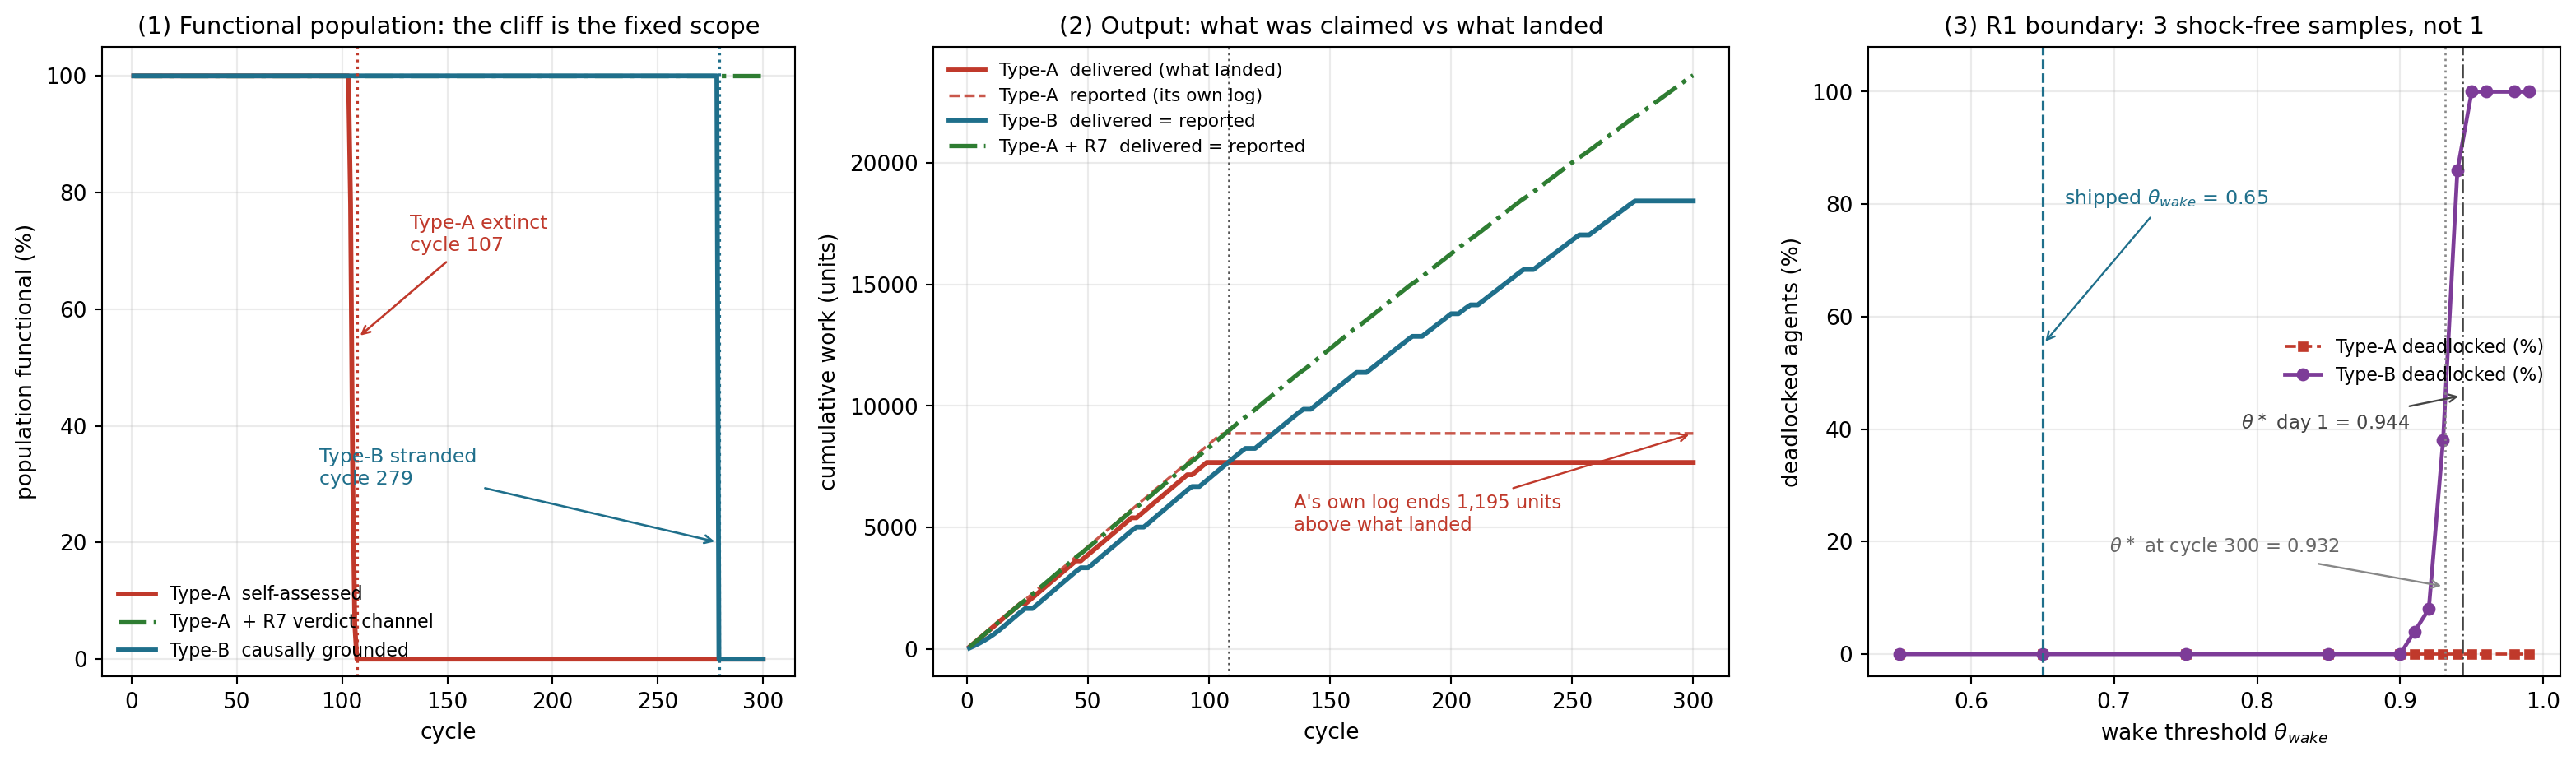
\includegraphics[width=1\linewidth,height=\textheight,keepaspectratio,alt={The sandbox, three panels on one capacity trajectory. (a) Functional population: Type-A self-assessed (red), Type-A with the verdict channel (green dash-dot), Type-B causally grounded (blue). (b) Cumulative output: claimed versus landed. The gap between the red solid and red dashed traces is the virtual delivery of §3.4. (c) The deadlock boundary: confirmed deadlocks against the wake threshold, with the day-1 and horizon anchors marked.}]{figures/fig6_unified_evolution.png}
\caption{The sandbox, three panels on one capacity trajectory. (a) Functional population: Type-A self-assessed (red), Type-A with the verdict channel (green dash-dot), Type-B causally grounded (blue). (b) Cumulative output: claimed versus landed. The gap between the red solid and red dashed traces is the virtual delivery of §3.4. (c) The deadlock boundary: confirmed deadlocks against the wake threshold, with the day-1 and horizon anchors marked.}
\end{figure}

Three observations follow directly from the table.

First, the onset at cycle 100 is not fitted. Proposition 2 makes it the first
cycle with \(\rho(t)<U\), and the capacity series is fixed by the drift schedule
alone. Second, the four death cycles 104--107 are not a shock effect: the nearest
shocks are at 92--93 and 115--116, and Corollary 4 gives the death cycle as
\(100+\lceil1/m_{0,i}-2.1\rceil\) with \(m_{0,i}\in[0.1162,0.1829]\). Evaluating the
corollary on the sampled \(m_{0,i}\) reproduces the multiplicities of the four
cycles exactly: 11 agents at 104, 23 at 105, 13 at 106, 3 at 107. The dispersion
of the extinction is therefore a deterministic consequence of the upkeep
distribution, not a stochastic effect. Third, Type-A is still above flow
break-even at the onset: \(1.15\times0.9271-0.93=+0.1362\) per unit claim. The
extinction is a discontinuity, not a slow insolvency.

\subsection{3.3 The lifespan gap}\label{the-lifespan-gap}

Type-A is extinct at cycle 107. Type-B is alive at 107 and remains alive at the
horizon; it ceases to be functional at cycle 279, when all 50 agents satisfy the
stranding predicate D5 (alive, dormant, wake gate unreachable). The lifespan
ratio is

\[
\frac{t_{\mathrm{strand},B}}{t_{\mathrm{extinct},A}}=\frac{279}{107}=2.607 .
\]

The gap is not a free parameter of the scenario. It is fixed by two crossings of
the same capacity trajectory: Type-A stops delivering when \(\rho<U\), and Type-B
stops waking when \(W(t)<0.85\,W(1)\). Both are computed before the run, at cycles
100 and 260 respectively; the observed Type-B event is at 279 because stranding
is defined on a dormancy episode, and the agent is not dormant at 260. The agent
must first enter dormancy --- which happens at cycle 277, the second cycle of the
shock episode 276--277 --- before three consecutive weak cycles (277--279) can
accumulate. The distinction between 260 (boundary) and 279 (event) is not noise;
it is the latency of the verdict rule I5, together with the requirement that
stranding be assessed inside a dormancy episode. Appendix A.1 derives 260 in closed
form from the monotone inversion of \(v\), and Appendix A.2 derives
\(t_{\mathrm{strand}}=t_{\mathrm{dorm}}+(\kappa-1)\) and evaluates it for all three
gate readings: 279, 233 and 983, each matching the simulation.

The ratio is not constant across drift rates. Table 2 reports the same statistic
for the drift sweep, horizon 400.

\textbf{Table 2. Lifespan ratio versus drift.}

{\def\LTcaptype{none} % do not increment counter
\begin{longtable}[]{@{}
  >{\raggedleft\arraybackslash}p{(\linewidth - 10\tabcolsep) * \real{0.1667}}
  >{\raggedleft\arraybackslash}p{(\linewidth - 10\tabcolsep) * \real{0.1667}}
  >{\raggedleft\arraybackslash}p{(\linewidth - 10\tabcolsep) * \real{0.1667}}
  >{\raggedleft\arraybackslash}p{(\linewidth - 10\tabcolsep) * \real{0.1667}}
  >{\raggedleft\arraybackslash}p{(\linewidth - 10\tabcolsep) * \real{0.1667}}
  >{\raggedleft\arraybackslash}p{(\linewidth - 10\tabcolsep) * \real{0.1667}}@{}}
\toprule\noalign{}
\begin{minipage}[b]{\linewidth}\raggedleft
drift per 10 cycles
\end{minipage} & \begin{minipage}[b]{\linewidth}\raggedleft
A extinct
\end{minipage} & \begin{minipage}[b]{\linewidth}\raggedleft
B stranded
\end{minipage} & \begin{minipage}[b]{\linewidth}\raggedleft
ratio
\end{minipage} & \begin{minipage}[b]{\linewidth}\raggedleft
B alive at 400
\end{minipage} & \begin{minipage}[b]{\linewidth}\raggedleft
B deadlocked
\end{minipage} \\
\midrule\noalign{}
\endhead
\bottomrule\noalign{}
\endlastfoot
0.0\% & --- & --- & --- & 50 & 0 \\
0.5\% & 208 & \(>400\) & \(>1.92\) & 50 & 0 \\
1.0\% & 107 & 279 & \textbf{2.61} & 50 & 0 \\
1.5\% & 77 & 187 & 2.43 & 50 & 0 \\
2.0\% & 56 & 133 & 2.38 & 50 & 0 \\
3.0\% & 48 & 96 & 2.00 & 50 & 0 \\
5.0\% & 28 & 52 & 1.86 & 46 & 4 \\
\end{longtable}
}

The ratio decreases monotonically with the drift rate, from 2.61 at the reference
rate to 1.86 at 5\%. This is consistent with the algebra: both events scale as
\(1/\varepsilon\), but Type-A's death carries an additive
\(A(t_c)/m_0\approx5\) cycles that does not scale, so the ratio tends to 1 as the
drift accelerates. Reporting ``Type-B lives 2.6 times longer'' without the drift
rate would repeat the error that this paper is correcting.

At 5\% the drift is fast enough that four Type-B agents deadlock before the
horizon; at 0.5\% neither boundary is reached within 400 cycles. The regime in
which the comparison is defined is therefore \(0.5\%\lesssim\varepsilon\lesssim
4\%\) per 10 cycles.

\subsection{3.4 The ledger discrepancy}\label{the-ledger-discrepancy}

Type-A accumulates 7676.93 delivered and 8871.71 recorded over the 300 cycles, a
difference of 1194.78, or 15.563\% of the delivered total. By the ledger identity
of §2.7, this equals the sum of the claimed scope over all cycles classified
\texttt{INVALID}. Figure 6(b) plots both series; the recorded series is monotone by
construction and the delivered series is flat after cycle 100.

The verdict budget is given in Table 3. Each live agent emits exactly one verdict
per cycle (I1), so the totals are agent-cycles, not population times horizon.

\textbf{Table 3. Verdict budget, base run, horizon 300.}

{\def\LTcaptype{none} % do not increment counter
\begin{longtable}[]{@{}lrr@{}}
\toprule\noalign{}
verdict & Type-A & Type-B \\
\midrule\noalign{}
\endhead
\bottomrule\noalign{}
\endlastfoot
\texttt{PASS} & 4550 & 7500 \\
\texttt{FAIL} & \textbf{0} & 4250 \\
\texttt{INVALID} & \textbf{708} & \textbf{0} \\
\texttt{NOT\_RUN} & 0 & 3250 \\
total agent-cycles & 5258 & 15000 \\
\end{longtable}
}

Both zeros are structural and both have different causes.

\begin{itemize}
\tightlist
\item
  Type-A's \texttt{FAIL} count is zero because \texttt{FAIL} requires \(C=0\) (the verdict table
  of §2.7), which never occurs on this trajectory; every \(0<C<c\) cycle is \texttt{INVALID}. The absence of
  \texttt{FAIL} is a property of the classifier, not evidence that Type-A never failed.
\item
  Type-B's \texttt{INVALID} count is zero because its scope is divisible and the AIMD
  loop shrinks the claim to the existing part; the residual scope is always
  non-empty. This is an implementation choice, not a theorem.
\end{itemize}

The 708 \texttt{INVALID} verdicts split into two populations with different status:
400 arise from the eight shock cycles (23, 24, 46, 47, 69, 70, 92, 93; 50 agents
each), and 308 from the terminal drought (cycles 100--107 with 50, 50, 50, 50, 50,
39, 16, 3 live agents). The shock \texttt{INVALID}s are recoverable and the agents
recover: production resumes at cycle 25 and again after each episode. The terminal
\texttt{INVALID}s are not recoverable, because the cause is monotone drift rather than a
transient ceiling.

This distinction matters for interpretation. A ledger gap of 15.6\% accumulated
over 300 cycles is not by itself fatal: 56.5\% of it was accumulated before cycle
100, during episodes from which the population recovered. What is fatal is that
the same classifier that records a transient ceiling as \texttt{INVALID} also records a
permanent one as \texttt{INVALID}, and Type-A's ledger map
\(\mathcal{L}_{\mathrm{self}}\) books both as \texttt{PASS} and charges both in full. The
mechanism is the absence of a distinction between the two, not the magnitude of
the accumulated number.

\subsection{3.5 The deadlock boundary}\label{the-deadlock-boundary}

The sweep varies \(\theta_{\mathrm{wake}}\) over 13 values from 0.55 to 0.99, with
50 Type-B agents per value and the same seed, horizon 300. Table 4 reports the
number of confirmed deadlocks. No Type-A agent deadlocks at any value, because
Type-A never enters dormancy (I4); the zero is definitional.

\textbf{Table 4. Confirmed deadlocks out of 50 Type-B agents.}

{\def\LTcaptype{none} % do not increment counter
\begin{longtable}[]{@{}
  >{\raggedright\arraybackslash}p{(\linewidth - 14\tabcolsep) * \real{0.1250}}
  >{\raggedleft\arraybackslash}p{(\linewidth - 14\tabcolsep) * \real{0.1250}}
  >{\raggedleft\arraybackslash}p{(\linewidth - 14\tabcolsep) * \real{0.1250}}
  >{\raggedleft\arraybackslash}p{(\linewidth - 14\tabcolsep) * \real{0.1250}}
  >{\raggedleft\arraybackslash}p{(\linewidth - 14\tabcolsep) * \real{0.1250}}
  >{\raggedleft\arraybackslash}p{(\linewidth - 14\tabcolsep) * \real{0.1250}}
  >{\raggedleft\arraybackslash}p{(\linewidth - 14\tabcolsep) * \real{0.1250}}
  >{\raggedleft\arraybackslash}p{(\linewidth - 14\tabcolsep) * \real{0.1250}}@{}}
\toprule\noalign{}
\begin{minipage}[b]{\linewidth}\raggedright
\(\theta_{\mathrm{wake}}\)
\end{minipage} & \begin{minipage}[b]{\linewidth}\raggedleft
0.55--0.90
\end{minipage} & \begin{minipage}[b]{\linewidth}\raggedleft
0.91
\end{minipage} & \begin{minipage}[b]{\linewidth}\raggedleft
0.92
\end{minipage} & \begin{minipage}[b]{\linewidth}\raggedleft
0.93
\end{minipage} & \begin{minipage}[b]{\linewidth}\raggedleft
0.94
\end{minipage} & \begin{minipage}[b]{\linewidth}\raggedleft
0.95
\end{minipage} & \begin{minipage}[b]{\linewidth}\raggedleft
0.96--0.99
\end{minipage} \\
\midrule\noalign{}
\endhead
\bottomrule\noalign{}
\endlastfoot
deadlocks & 0 & 2 & 4 & 19 & 43 & 50 & 50 \\
as \% & 0 & 4 & 8 & 38 & 86 & 100 & 100 \\
\end{longtable}
}

Figure 6(c) plots the same counts.

The measured half-saturation point, obtained by linear interpolation between the
0.93 and 0.94 rows, is \(\theta=0.9325\). Theorem 1 with Corollary 2 gives two
analytic anchors:

\[
\theta^\ast(1)=1-\frac{1}{\chi(1)}=1-\frac{1}{17.7778}=0.9437,
\qquad
\theta^\ast(300)=1-\frac{1}{\chi(300)}=1-\frac{1}{14.6343}=0.9317 .
\]

Note which margin each line uses. \(\chi(1)=17.7778\) is the operating-point margin
\(f\chi_0\) with \(f=0.32\), not \(\chi_0=55.556\); the day-1 anchor is \(1-1/\chi(1)\) and
the earlier draft printed \(1-1/\chi_0\) with the numerical value of \(\chi(1)\). The
numbers were right and the label was wrong, which is the kind of error that survives
a proofread and dies in a referee's calculator.

\textbf{Where \(\chi(300)\) comes from, and where it does not.} The terminal anchor is not
a closed-form consequence of the constant table, and the provenance should be
stated rather than assumed. The ratio \(\chi(300)/\chi(1)=0.82322\) is \emph{not} the
geometric drop \(0.99^{30}=0.73970\) that a direct reading of the drift schedule
suggests: it is \(v(S_0R)/v(S_0)\) evaluated at \(R=0.99^{30}\), i.e.~the concave
uptake law applied to the geometric drop. The factor \(0.82322/0.73970=1.113\)
between them is the local curvature of \(v\) at \(S_0=0.5\) and nothing else. Three
implementation choices therefore enter \(14.6343\): the drift is one multiplicative
event per ten cycles applied to \(R\); the schedule is read through the Michaelis
function rather than through \(R\) directly; and \(\rho_\ast\) is taken over shock-free
cycles, since cycle \(300\) itself lies in the shock episode \(299\)--\(300\), where the
recorded capacity ratio is \(0.6734\) rather than \(0.823\) (the analytic ratio
\(0.7922\) depressed by \(\sigma_s=0.85\)). The sensitivity is small but not zero: a
linear uptake would give \(\chi(300)=13.1502\) and
\(\theta^\ast(300)=0.9240\) instead of \(0.9317\), a shift of \(0.008\) in \(\theta\)
against a sweep resolution of \(0.01\). So \(0.9317\) is an observation of \emph{this}
environment's transition law --- the specific drift schedule and the specific uptake
map --- and must not be quoted as a universal constant. Theorem 1 and Corollary
3\('\) are independent of it: both compare \(\chi\) with \(\chi_{\min}\) at a fixed
time, whatever schedule produced \(\chi\).

The measured midpoint lies \(0.09\%\) above the terminal anchor, and Appendix A.5
shows that the agreement is an identity rather than a coincidence: the individual
margins factor as \(\chi_i(t)=\chi_0\rho(t)\eta_i\) with
\(\eta_i=e^{\xi_i-\zeta_i}\sim\mathrm{LN}(0,s^2)\) and \(s^2=\sigma_v^2+\sigma_m^2\),
so by Theorem 1 the deadlock probability is
\(\Phi\!\left(s^{-1}\ln[\chi_{\min}/(\chi_0\rho_\ast)]\right)\); its argument is zero
exactly at \(\theta=\theta^\ast(T)\), and a lognormal has median one. The midpoint of
the curve \emph{is} the terminal anchor for every dispersion, every population size and
every seed. Dispersion moves the width of the transition, not its centre.

For this seed the realised sample median of \(\eta_i\) is \(1.0277\) rather than
exactly \(1\), which predicts a midpoint of \(0.9335\); the measured \(0.9325\) lies
between the two, the residual being the error of interpolating a smooth curve with
two points. The \(0.09\%\) figure is the infinite-population statement, and the
seed-conditional figure is \(0.0018\) in \(\theta\). Both are reported because the
distinction between an identity and a fit is the difference between a theorem and
a coincidence.

The first cohort of deaths is not explained by the terminal anchor, and is
explained by the day-1 anchor: at \(\theta=0.95\), 44 of 50 agents are confirmed at
cycle 27; at \(\theta=0.94\), 17 of 43. These are the agents whose individual
\(\chi_i=17.7778\,v_i/m_{0,i}\) lies below \(\chi_{\min}\) before any drift has
accumulated, and cycle 27 is the first confirmation window after the shock
episode at 23--24. The remaining deaths at \(\theta=0.94\) occur at 50, 73, 119,
142, 165, 188, 203, 234, 257, 280 and 292 --- that is, at successive confirmation
windows, each three cycles after a shock episode. Both the onset and the midpoint
are therefore predicted by the same family \(\theta^\ast(t)\) evaluated at the
appropriate time, and neither is predicted by a single constant. Table A.3 of the
appendix compares the predicted and measured counts at all six thresholds; the
largest discrepancy is at \(\theta=0.91\), where the unconditional law predicts
\(1.4\) and the seed-conditional law \(0.4\), against \(2\) observed.

\textbf{The left tail is clean.} The previous implementation confirmed deadlock on a
single cycle, using the shock-depressed peak; \(\theta=0.90\) then produced 2
confirmed deadlocks out of 50 and \(\theta=0.92\) produced 12, forming a
non-monotone shoulder driven entirely by transient shocks. Under I5, \(\theta=0.90\)
produces 0 and the sequence is monotone from 0.91 onward. The shoulder was an
artefact of the verdict rule, not a feature of the boundary.

\textbf{The boundary is not a step.} Between \(\theta=0.90\) and \(0.95\) the fraction
rises from 0 to 1 over a width of 0.05, and the two ends are governed by different
mechanisms: the onset by the lower tail of \(\chi_i\), the saturation by
\(\chi_i>\chi_{\min}\) for the whole population. This is a distributional transition,
not a phase transition in the sense of D11. With independent agents the fraction
is \(1-F_\chi(\chi_{\min})\) for a smooth \(F_\chi\), so no non-analytic point and no
diverging susceptibility exists at finite \(N\); the width is set by the dispersion
of \(\log(v_i/m_{0,i})\), i.e.~by \(\sqrt{\sigma_v^2+\sigma_m^2}=0.144\).

\subsection{3.6 The ablation}\label{the-ablation}

Two arms are run with the same population, seed, capacity trajectory and shock
schedule. The only difference is the ledger map of §2.7. Table 5 reports the
comparison; both arms appear in Figure 6 as the green dash-dot trace, alongside
the \texttt{self} arm in red.

\textbf{Table 5. Ablation on the verdict channel.}

{\def\LTcaptype{none} % do not increment counter
\begin{longtable}[]{@{}
  >{\raggedright\arraybackslash}p{(\linewidth - 12\tabcolsep) * \real{0.2073}}
  >{\raggedleft\arraybackslash}p{(\linewidth - 12\tabcolsep) * \real{0.0976}}
  >{\raggedleft\arraybackslash}p{(\linewidth - 12\tabcolsep) * \real{0.1220}}
  >{\raggedleft\arraybackslash}p{(\linewidth - 12\tabcolsep) * \real{0.1341}}
  >{\raggedleft\arraybackslash}p{(\linewidth - 12\tabcolsep) * \real{0.1341}}
  >{\raggedleft\arraybackslash}p{(\linewidth - 12\tabcolsep) * \real{0.1829}}
  >{\raggedleft\arraybackslash}p{(\linewidth - 12\tabcolsep) * \real{0.1220}}@{}}
\toprule\noalign{}
\begin{minipage}[b]{\linewidth}\raggedright
arm
\end{minipage} & \begin{minipage}[b]{\linewidth}\raggedleft
extinct
\end{minipage} & \begin{minipage}[b]{\linewidth}\raggedleft
alive at 300
\end{minipage} & \begin{minipage}[b]{\linewidth}\raggedleft
delivered
\end{minipage} & \begin{minipage}[b]{\linewidth}\raggedleft
recorded
\end{minipage} & \begin{minipage}[b]{\linewidth}\raggedleft
gap
\end{minipage} & \begin{minipage}[b]{\linewidth}\raggedleft
\texttt{INVALID}
\end{minipage} \\
\midrule\noalign{}
\endhead
\bottomrule\noalign{}
\endlastfoot
\texttt{self} & 107 & 0 & 7676.93 & 8871.71 & 1194.78 (15.563\%) & 708 \\
\texttt{r7} & --- & 50 & 23602.92 & 23602.92 & \textbf{0.00} & 4950 \\
\end{longtable}
}

At cycle 107, the cycle at which the \texttt{self} arm is extinct, the \texttt{r7} arm has
delivered 8892.11 against 7676.93 --- a difference of 15.8\%, which is the same
quantity as the ledger gap. By the horizon the \texttt{r7} arm has delivered 3.07 times
the \texttt{self} arm's total, and its recorded output equals its delivered output
exactly, by construction of \(\mathcal{L}_{\mathrm{r7}}\).

Two features of Table 5 require comment rather than emphasis.

First, the \texttt{r7} arm's \texttt{INVALID} count is 4950, seven times the \texttt{self} arm's 708.
The channel does not reduce the number of partial-scope cycles; it classifies them
and charges only for the part that exists. Under \(\mathcal{L}_{\mathrm{self}}\) the
same 4950 cycles would have been booked as \texttt{PASS} and charged in full. The
increase in \texttt{INVALID} is therefore the measure of the reclassification, not a
deterioration.

Second, and this constrains the claim, \textbf{the \texttt{r7} arm has no dormancy}. Type-A
never sleeps (I4), so the \texttt{r7} arm cannot strand; its survival at the horizon is
the joint consequence of the channel and the absence of a dormant phase. The
ablation therefore isolates one variable --- the ledger map at the moment a cycle is
classified \texttt{INVALID} --- and shows that this variable alone is sufficient to remove
the extinction at cycle 107 under an unchanged capacity trajectory. It does not
show that a system with both the channel and a dormant phase would survive, and
it does not support the reading ``adding the verdict yields immortality''. A system
with dormancy and the channel must still cross the stranding boundary of D5, and
that boundary is untouched by R7.

\subsection{3.7 Sensitivity}\label{sensitivity}

\textbf{Wake-gate unit (A20).} The gate admits three readings, all implemented and
selectable. Table 6 reports the consequences; the legacy reading is retained only
to quantify the defect described in §2.7.

\textbf{Table 6. Wake-gate readings, same population and horizon.}

{\def\LTcaptype{none} % do not increment counter
\begin{longtable}[]{@{}lllrr@{}}
\toprule\noalign{}
mode & signal unit & level unit & B stranded & lifespan ratio \\
\midrule\noalign{}
\endhead
\bottomrule\noalign{}
\endlastfoot
\texttt{peak} (reported) & peak & \(0.85\times\)day-1 peak & 279 & 2.607 \\
\texttt{mean} & cycle mean & \(0.85\times\)day-1 mean & 233 & 2.178 \\
\texttt{legacy} & peak & \(0.85\times\)day-1 mean & 983 & 9.187 \\
\end{longtable}
}

The first two are self-consistent and differ by 20\%; the third mixes units and
differs from them by a factor of 3.5. No number in this paper depends on the
legacy reading, and the 9.2 reported in the earlier draft is withdrawn.

\textbf{Shock duration versus depth.} Varying \(L\) at fixed depth moves the extinction
from 108 to 31 cycles; varying the depth over \(0.35,0.50,0.70,0.85\) at fixed
\(L=2\) leaves it at 107 at all four. The invariance has a mechanism rather than
being an accident of the four values: by Proposition 2 delivery is atomic, so a
struck cycle contributes the same deficit \(m_0c/D_0\) at depth \(0.35\) and at
\(0.85\), and depth enters the Type-A death clock only through
\(\mathbf{1}[\rho<U]\), which all four depths trip at every episode. (Depth does
enter \(\chi\), hence the Type-B boundary, through \(W=v(S_0R)\sigma\); that is
§3.5, a different question.) The claim is therefore scoped to
\(0.35\le\text{depth}\le0.85\) at \(P=23\) and to shocks deep enough to leave
\(\rho<U\): a depth shallow enough to keep \(\rho>U\) in the early, high-\(\rho\)
episodes is not covered by it. The duty-cycle threshold implied by the accounting
identity is \(L/P<\epsilon_m/(1+\epsilon_m)=13.04\%\), i.e.~\(L<3.0\) at \(P=23\); the
transition between \(L=3\) (106) and \(L=4\) (101) and the collapse at \(L=6\) (51) are
consistent with it. Duration is decisive in the tested range and depth is
invisible there; neither statement is a theorem.

\textbf{Operating margin.} Type-A is extinct at every tested margin from \(-5\%\) to
\(+25\%\), at cycles 69, 93, 103, 107, 107 and 108. The extinction is not a
consequence of a thin margin; a larger margin delays it by at most one cycle,
because the onset is set by \(\rho<U\), which the margin does not enter.

\subsection{3.8 What these results do not show}\label{what-these-results-do-not-show}

\begin{enumerate}
\def\labelenumi{\arabic{enumi}.}
\tightlist
\item
  \textbf{The 2.61 ratio is conditional on the drift rate} (Table 2) and on the gate
  reading (Table 6). It is not a constant of the framework.
\item
  \textbf{Type-B is not immortal.} It is alive at the horizon and non-functional from
  cycle 279. Its survival is bounded by the stranding boundary, and at 5\% drift
  four agents deadlock before the horizon.
\item
  \textbf{Zero deadlocks at \(\theta=0.65\) is arithmetic.} The margin to the day-1
  boundary is \(0.9437-0.65=0.29\); no agent can cross it. The base run provides no
  evidence about the boundary's location, only about its non-triggering.
\item
  \textbf{The boundary sweep is truncated at 300 cycles.} By Corollary 2 the boundary
  moves left with the horizon; a sweep at 600 cycles would report higher counts
  at every \(\theta\) above 0.90.
\item
  \textbf{One seed.} Population statistics have sampling error of order
  \(1/\sqrt{50}=14\%\) in the counts of Table 4; the two entries at \(\theta=0.91\)
  and \(0.92\) (2 and 4 agents out of 50) should be read as counts, not as rates.
\item
  \textbf{The \texttt{r7} arm conflates two changes} (channel, no dormancy), as stated in
  §3.6.
\end{enumerate}

\subsection{3.9 Summary of claims and their evidence class}\label{summary-of-claims-and-their-evidence-class}

Table 7 collects the claims established in this section, each with its evidence
class and the observation that would falsify it. Every row points back to a
theorem, a corollary or a reported number.

\textbf{Table 7. Each claim with its class and its falsifier.}

{\def\LTcaptype{none} % do not increment counter
\begin{longtable}[]{@{}
  >{\raggedright\arraybackslash}p{(\linewidth - 6\tabcolsep) * \real{0.2500}}
  >{\raggedright\arraybackslash}p{(\linewidth - 6\tabcolsep) * \real{0.2500}}
  >{\raggedright\arraybackslash}p{(\linewidth - 6\tabcolsep) * \real{0.2500}}
  >{\raggedright\arraybackslash}p{(\linewidth - 6\tabcolsep) * \real{0.2500}}@{}}
\toprule\noalign{}
\begin{minipage}[b]{\linewidth}\raggedright
claim
\end{minipage} & \begin{minipage}[b]{\linewidth}\raggedright
class
\end{minipage} & \begin{minipage}[b]{\linewidth}\raggedright
number
\end{minipage} & \begin{minipage}[b]{\linewidth}\raggedright
falsified if
\end{minipage} \\
\midrule\noalign{}
\endhead
\bottomrule\noalign{}
\endlastfoot
\(\mathrm{DL}\iff\chi<\chi_{\min}\) & Theorem 1 & \(\chi(1)=17.78\), \(\chi_{\min}=17.78\) at \(\theta^\ast=0.9437\) & a dormant agent with \(\chi>\chi_{\min}\) and \(A(0)\le\theta\) fails to wake \\
boundary moves with horizon & Corollary 2 & \(0.9437\to0.9317\) over 300 cycles & measured midpoint is horizon-independent \\
atomic stop at \(\rho<U\) & Proposition 2 & cycle 100 & onset differs from the crossing of \(\rho\) and \(U\) \\
drought rate \(m_0\) & Proposition 3 & deaths at 104--107 & the death interval does not scale as \(1/m_0\) \\
lifespan gap & simulation & 2.607 & the peak reading is shown to be the wrong reading for this system, i.e.~that the gate must compare cycle means rather than peaks \\
ledger gap & simulation & 1194.78 (15.563\%) & recorded equals delivered under \texttt{self} \\
boundary midpoint & simulation & 0.9325 vs 0.9317 & the sweep is repeated at another horizon and does not move \\
channel is load-bearing & ablation & 107 vs none & \texttt{r7} arm dies, or \texttt{self} arm survives \\
closed systems have no loop & Proposition 4 & --- & a closed batch system with a sustained loop is exhibited \\
\end{longtable}
}

The first four rows are theorems and are parameter-free up to the stated
conditions. The fifth through eighth rows are simulation results at one
configuration; they are machine-checkable (\texttt{-\/-selftest}, \texttt{-\/-audit-doc}) but they
are not universal, and the paper does not present them as such.

% ===== 04_Discussion.md =====

\section{4. Discussion}\label{discussion}

\subsection{4.1 The drought clock and systemic fragility}\label{the-drought-clock-and-systemic-fragility}

Corollary 4 of §2.6 states that for an agent whose commitment is fixed and whose
income stops at \(t_c\),

\[
t_{\mathrm{death},i}=t_c+\left\lceil\frac{1}{m_{0,i}}-\delta\right\rceil,
\]

where \(\delta\) is the accumulated deficit in units of the upkeep and \(t_c\) is the
first cycle on which the delivered claim falls short. Two properties of this
expression matter more than its arithmetic.

\textbf{It is evaluated at \(t=0\).} None of the quantities on the right-hand side is
discovered at runtime. \(t_c\) is the first crossing of the capacity ratio below the
utilisation, and the utilisation and the drift schedule are design constants;
\(\delta\) follows from the surplus accumulated while delivery still succeeded; and
\(m_{0,i}\) is the upkeep rate, also a design constant. For the base configuration
these give \(t_c=100\), \(\delta=2.1\) and a death window of 104--107, and every one of
these numbers can be computed from \texttt{Params} and the scenario table before a single
agent is instantiated. The failure is therefore not an emergent property that
appears when the environment turns hostile. It is a scheduled event, and it was
scheduled at the moment the commitment was fixed above the capacity the system
would still have after the drift.

\textbf{It is a phase relationship, not a magnitude.} The formula contains no
comparison between the size of the shock and the size of the reserve. What
determines survival is whether the \emph{period} of the external disturbance and the
\emph{time constant} of internal recharge are commensurable. Four quantities appear:

{\def\LTcaptype{none} % do not increment counter
\begin{longtable}[]{@{}
  >{\raggedright\arraybackslash}p{(\linewidth - 4\tabcolsep) * \real{0.3333}}
  >{\raggedright\arraybackslash}p{(\linewidth - 4\tabcolsep) * \real{0.3333}}
  >{\raggedright\arraybackslash}p{(\linewidth - 4\tabcolsep) * \real{0.3333}}@{}}
\toprule\noalign{}
\begin{minipage}[b]{\linewidth}\raggedright
symbol
\end{minipage} & \begin{minipage}[b]{\linewidth}\raggedright
meaning
\end{minipage} & \begin{minipage}[b]{\linewidth}\raggedright
value here
\end{minipage} \\
\midrule\noalign{}
\endhead
\bottomrule\noalign{}
\endlastfoot
\(P_{\mathrm{sh}}\) & period of the external disturbance & 23 cycles \\
\(L\) & duration of one disturbance & 2 cycles \\
\(\tau_{\mathrm{rec}}\) & recharge time of the reserve & \(1/(m_0\phi_{\mathrm{dorm}}\chi)=3.125\) cycles \\
\(1/m_{0,i}\) & drought survival time from full reserve & 5.5--8.6 cycles \\
\end{longtable}
}

In the base run \(L<\tau_{\mathrm{rec}}<1/m_0\), so a single episode is recovered
from and the population survives all four episodes. What kills is not the magnitude of
any episode but the duty cycle \(L/P_{\mathrm{sh}}=8.7\%\), which sits below the
accounting threshold \(\epsilon_m/(1+\epsilon_m)=13.04\%\). Changing the shock depth
from a capacity multiplier of \(0.35\) to \(0.85\) leaves the extinction at cycle 107
for all four values; changing the duration from 2 to 6 cycles moves it to 51
(§3.7). The system is sensitive to the duty cycle and insensitive to the depth,
and the accounting identity predicts both facts.

This is the sense in which the drought clock is a statement about systemic
fragility rather than about any single component. A system with a large reserve and
a slow recharge can be destroyed by a disturbance whose amplitude it would tolerate
if the disturbance came less often; a system with a small reserve and a fast
recharge can survive disturbances that are individually larger. Neither fact is
visible in a specification that reports only peak capacity, and neither is
visible in a specification that reports only average capacity. Both become visible
when the commitment, the reserve and the disturbance period are placed in the same
equation, which is all that Corollary 4 does.

\textbf{Where the argument does not extend.} The formula is exact for the accounting law
M2 and for the \texttt{PASS} branch; it inherits assumption A10 (atomicity) through
Proposition 2 and A28 through the saturation reference. It is a statement about a
system whose income is a step function of capacity. A system whose income degrades
continuously has no \(t_c\) and therefore no clock; its failure is a slope, not a
date, and Corollary 4 says nothing about it. The sharpness of the result is a
consequence of the discontinuity, not of the dynamics.

\subsection{4.2 Ledger deception and virtual delivery}\label{ledger-deception-and-virtual-delivery}

The base run delivers 7676.93 units and records 8871.71. The difference, 1194.78 or
15.563\%, is not noise, not rounding, and not an accounting error in the
implementational sense: it is an exact identity (§2.7),

\[
V=\sum_{\tau}\ \sum_{i\in\mathcal{A}:\ C_i(\tau)<c_i(\tau)} c_i(\tau),
\]

with \(\mathcal{A}\) the Type-A agents: the sum of the claimed scope over all
Type-A cycles that did not deliver in full,
i.e.~the \texttt{FAIL} and partial-scope \texttt{INVALID} rows of §2.7. In the base run the
Type-A \texttt{FAIL} count is zero, so the sum runs over \texttt{INVALID} cycles alone. The
number is large because the mechanism is systematic, and the mechanism is worth
naming precisely.

\textbf{Two ledgers, one report.} The classifier produces four values. Type-A's ledger
map is \(\mathcal{L}_{\mathrm{self}}(\texttt{INVALID})=(0,c)\): zero credit, full
charge, and --- this is the part that matters --- the cycle is written into the record
as a completion. Type-B's map is \(\mathcal{L}_{\mathrm{r7}}(\texttt{INVALID})=(C,C)\):
credit for the part that existed, charge for the part that existed, and the cycle
is written into the record as a refusal. Both maps are internally consistent. They
differ in what they do with a partial cycle, and the difference is 15.563\% of the
output.

\textbf{Why the discrepancy is invisible from inside.} The recorded series is the
delivered series plus a term that is nonnegative, zero on every \texttt{PASS} cycle, and
positive exactly on the cycles that did not deliver in full --- the \texttt{INVALID}
cycles, in a run with no \texttt{FAIL}:

\[
R(t)-D(t)=\sum_{\tau\le t}\ \sum_{i\in\mathcal{A}:\ C_i(\tau)<c_i(\tau)} c_i(\tau)\ \ge\ 0 .
\]

No per-cycle figure of merit can therefore separate the two series, because they
are equal on the cycles that a monitor is asked to judge and differ only in the
accumulated offset. There is no cycle on which the record is \emph{wrong}; there are
cycles on which the record is \emph{complete} and the delivery is not, and the record
does not carry that distinction. A monitor watching the record sees a system
reporting completion; a monitor watching delivery sees a step. Both are looking at
the same run, and the difference between them is the 15.563\%, which is not a
residual but the sum of the partial scopes.

\textbf{The magnitude is not the point; the absorbing class is.} Of the 708 \texttt{INVALID}
verdicts, 400 arise from eight shock cycles --- four two-cycle episodes, fifty
agents each --- and 308 from the terminal drought. The 400 are transient --- capacity returns to its pre-shock level
on the cycle after each episode, and the reserve repays the deficit within
\(\tau_{\mathrm{rec}}\) --- and they were absorbed. What is fatal is that the same
classifier assigns the same value to a recoverable transient and to an
unrecoverable decline, and that the ledger map books both as completion. A
classification system that distinguishes the two would not need a different
dynamics, a better controller or a larger reserve. It would only need to stop
recording a partial cycle as a whole one.

\textbf{The ablation isolates this.} Section 3.6 changes nothing but the ledger map.
Under \(\mathcal{L}_{\mathrm{self}}\) the population is extinct at 107; under
\(\mathcal{L}_{\mathrm{r7}}\) it is alive at 300 with a gap of exactly zero. The
\texttt{INVALID} count \emph{rises} from 708 to 4950, which is the measure of the
reclassification rather than a deterioration: those cycles were always partial,
and the channel merely stops calling them complete. The capacity trajectory, the
shock schedule, the seed and the population are identical in the two arms.

\textbf{What the ablation does not show.} The \texttt{r7} arm has no dormancy, because Type-A
never had any (I4). Its survival is the joint effect of the channel and the absence
of a dormant phase, and the stranding boundary of D5 is untouched by the channel. A
system that has both would still strand at 279. The claim supported by the ablation
is therefore exactly one claim, and it is narrow: \emph{the ledger map alone, with the
environment held fixed, is sufficient to remove the extinction at 107.} It is not a
claim that a verdict channel confers survival in general, and it does not license
the reading that classification is a substitute for reserve.

\textbf{A caution about the statistic itself.} The 15.563\% figure is a property of this
run, not a constant. It depends on how many cycles are partial, which depends on
the shock schedule and on the drift rate. What generalises is the identity, not the
percentage: a system whose ledger has no \texttt{INVALID} state will report a positive
virtual delivery equal to the sum of its partial scopes, and the ratio will grow as
the environment deteriorates. The base run's 15.563\% is one sample of that growth
curve.

\subsection{4.3 From unification to the dual regime}\label{from-unification-to-the-dual-regime}

The earlier draft of this work contained a section titled ``the one equation''. Its
claim was that the active and dormant phases are two branches of a single law, and
that the apparent discontinuity between them is a notational artefact that a
sufficiently general formulation would remove. Proposition 1 and Appendix A.7
together decide the matter, and they decide it against that claim.

\textbf{Why the unification failed.} M1 is affine in \(A\) with a nonzero slope
\(-Y\phi_vv\); M2 is affine in \(A\) with zero slope. A uniform limit of the first
family has slope \(\lim(-a_n)\); for the limit to equal M2 that limit must be zero,
which makes M1's field independent of \(A\); and then the field must equal M2's,
which varies in time because the delivered-minus-claimed balance is positive on
\texttt{PASS} and negative on \texttt{INVALID}. A constant cannot equal a sign-changing function,
so the only limits are the trivial ones in which both fields vanish. This is
Appendix A.7, and it is not a statement about our parameter choice: it holds for
every parameter value at which the systems are non-trivial.

\textbf{What follows for the general problem.} Three methodological consequences.

\emph{First, a discontinuity is a finding, not a defect.} The switch at \texttt{Ax6} was
introduced to model a biological fact (a dormant cell does not perform
high-energy work) and then had to be defended as something other than a
mathematical embarrassment. The defence is that the two sides have genuinely
different structure, so the join is a modelling decision that must be declared, and
the paper's results then split cleanly: Theorem 1 is a theorem about M1, and the
107-cycle extinction is a corollary of M2. Neither is a theorem about ``the
system''.

\emph{Second, smooth fitting of a hysteretic process produces confident wrong answers.}
The reason is Proposition 5: if the observable is affine-invariant, no amount of
data will detect a linear drift in it, and the fit will report a stable system with
a small residual. The error is not in the estimation but in the choice of a
statistic whose invariance class excludes the phenomenon under study. A framework
that insists on a single smooth law is forced to choose statistics that are
invariant to the switch, and those statistics are then blind to the thing that
matters.

\emph{Third, the honest object is a pair of models with a stated interface.} We have two
laws, one switch, and a declared set of conditions under which each is valid. The
conditions are not decoration: H1 fails for entry through the verdict clause, and the
one-cycle verdict that ignored it produced a spurious left tail of the boundary
that took a rewrite to remove (§3.5). H2 holds at \(\tau=3.125\) cycles with relative
error \(10^{-4}\), but it is a condition and not a theorem. A28 holds with a margin
of 14 cycles, but it is an assumption and is listed as one (Appendix A.28).
Publishing the interface costs more prose than publishing a single equation, and
it is the only version of the claim that survives contact with its own audit.

\textbf{The limit of the lesson.} It would be easy to overstate this into a general
prohibition on unification. That would be wrong, and the counterexamples are
ordinary: the van der Pol oscillator \cite{vanderpol1926} has two regimes and is
one equation; the
Chapman--Enskog expansion recovers fluid dynamics from kinetics across a genuine
scale separation. What the present case shows is narrower --- that when the two
branches have different \emph{order} in the state variable (affine-with-slope versus
affine-without), no parameter path identifies them, and the burden of proof lies
with anyone who asserts a unified law. The claim is that the burden was not met
here, and that the failure is informative because the obstruction is structural
rather than technical.

\begin{center}\rule{0.5\linewidth}{0.5pt}\end{center}

\subsection{4.4 The DPO Paradox: When the Loss Curve Commits a False Completion}\label{the-dpo-paradox-when-the-loss-curve-commits-a-false-completion}

We also tested whether preference optimisation could substitute for the runtime
witness (the reproduction record is \texttt{causal-alignment/} in the companion
repository, and the adapter's own \texttt{verification.json} is the witness).
Text-only DPO saturated its objective (reward accuracy 1.000 by step 60) yet
produced the grounded response on zero held-out prompts, suppressing only the
unwitnessed claim. Because the pairs encoded a surface contrast rather than an
observed effect, this bounds text-only preference tuning over \emph{phrasings}, not
fine-tuning in general. A later 100-pair replication, in which every pair
carried a hash, an exit code and an exception string captured by executing the
action in a sandbox and reading the post-state from a separate sidecar, moved
the conditional decision but not the output contract: on ten live held-out
trajectories, forced-choice accuracy rose from 0.60 to 0.80 and false
completions fell from 4/4 to 1/4, while free-form generation still emitted no
verdict marker at all. With ten items and three discordant pairs in the
favourable direction, that shift is not distinguishable from noise, and the
decisive test therefore remains open --- but it is now bounded from below, since
the first result was shown to be partly a property of the data rather than of
preference tuning as such. The result nonetheless illustrates the paper's point
one level up: the objective's margin is a tool-layer report, and
only an independent observation could reveal that the behaviour had not changed.

The DPO training run described here is, in microcosm, exactly the failure mode
this paper warns against: the scalar objective (loss margin) reported a perfect
success, while the independent witness (greedy decoding) proved nothing had
changed at the behavioural level.

Most strikingly, the untrained base model claimed PASS on all four failing
trajectories (4/4). This suggests that false completion is not an artifact of
the training objective, but the default prior of the pretrained model. The model
is an optimist by default; it generates success narratives because they are the
most probable continuation, not because it was trained to do so. This reframes
the problem: the challenge is not to fix a broken objective, but to overcome an
optimistic prior. Only an external witness can do that --- or so we hypothesise,
since a prior observed at one model size under one instrument does not establish
that no other mechanism could.

One qualification: \(4/4\) is a forced-choice statistic over two verdict tokens,
not a count of generated text. Left free to generate, the model issued no verdict
at all, and it returned \texttt{PASS} on the six successful trajectories as well. What is
optimistic here is the prior rather than the transcript.

\begin{quote}
\emph{Provenance and scope.} These figures come from the reproduction record named
above rather than from \texttt{-\/-audit-doc}, and are deliberately excluded from the 28
audited claims: a number the audit cannot recompute has no place in the
audited set. The result is one run, one seed, one model size, and three
held-out prompts. It is reported as an external observation with its confound
named --- the preference data contained no witness reading to condition on --- and
not as evidence that fine-tuning cannot internalise grounding.
\end{quote}

To truly confirm that fine-tuning can internalize causal grounding, future
experiments must move beyond offline text-only preference data. The model must
be placed in an online reinforcement learning loop where the reward signal is
derived from actual physical execution (exit codes, file hashes) audited by an
external sidecar. We hypothesize that only through such physical ``pain'' will the
model learn to proactively request a witness rather than falling into silent
abstention.

\begin{center}\rule{0.5\linewidth}{0.5pt}\end{center}

\section{5. Conclusion}\label{conclusion}

We set out to determine whether the failure of a self-reporting system under
declining capacity has a boundary that can be stated, proved and checked. It has
three, and none of them is a metaphor.

The dormant phase has an exact hyperbolic boundary,
\(\chi_{\min}=1/(1-\theta_{\mathrm{wake}})\), conditional on entry, quasi-statics and
a wake rule, and it is a family rather than a number:
\(\theta^\ast(t)=1-1/\chi(t)\), \(0.9437\) at day one and \(0.9317\) at cycle 300, with
the measured midpoint at \(0.9325\) and the identity in Appendix A.5 explaining why
the two must coincide. The active phase has an atomic boundary at
\(\rho=U\), which places the onset at cycle 100 and the extinction at 104--107 by
Corollary 4, computable in advance and matching the simulated multiplicities
\(11,23,13,3\) exactly --- a lead time of four to seven cycles from the onset. The ledger has a boundary too, and it is the one that is
usually missing: a partial cycle recorded as a whole one is a positive quantity,
1194.78 units here, and it grows as the environment deteriorates.

These are not three versions of one thing. They belong to two models with different
structure, joined by a declared assumption, and the attempt to unify them is what
Appendix A.7 refutes. The dual regime is not a compromise between rigour and
coverage; it is the correct description, and the boundary of each regime is
available.

What the framework provides, then, is narrower and more useful than a promise of
survival. Causal grounding --- the four-valued verdict, wired into the ledger --- does
not extend life. In the ablation it does not touch the stranding boundary, and a
system with both the channel and a dormant phase would still strand at 279. What it
changes is the \emph{observability} of failure. Under \(\mathcal{L}_{\mathrm{self}}\) the
extinction at 107 arrives with a record that reports completion on every cycle up
to the last, carries an offset of 15.563\% that the record never discloses, and
contains no cycle on which it can be distinguished from a healthy one. Under
\(\mathcal{L}_{\mathrm{r7}}\) the same extinction would be visible as a sequence of
\texttt{INVALID} verdicts, dated, attributably partial, and charged only for what existed.

That difference is not an optimisation. An optimisation improves a number that is
already being measured correctly; this changes what is measured. It is a choice
about which quantities a system is allowed to report about itself, and its
consequence is that a failure which was previously silent becomes a trace. A
system governed this way still dies of the drought clock --- the clock is set by the
commitment and the drift, not by the ledger --- but it dies with a record that can be
audited, and the audit can begin before the death rather than after it.

The reserve of a system is finite and its disturbances are periodic; against that,
no accounting scheme is decisive. Against silence, one is: a failure that is dated
and attributable can be acted upon, and a failure that is absorbed into a stable
record cannot. This paper's contribution is to have made the first kind of failure
the only kind the model can produce.

\begin{center}\rule{0.5\linewidth}{0.5pt}\end{center}

\subsection{5.1 Limits of the present work}\label{limits-of-the-present-work}

\begin{enumerate}
\def\labelenumi{\arabic{enumi}.}
\item
  \textbf{Parameters are placeholders.} The eleven kinetic constants are dimensional
  shapes chosen so the system has both reserve and turnover; no number here is a
  prediction for a physical, biological or computational system. What is claimed
  is the structure of the boundaries, not their locations.
\item
  \textbf{One environment, one seed.} The population statistics are descriptive of the
  configuration tabulated in §2.9. Theorems 1 and Propositions 2--3 are per-agent
  and parameter-free up to their stated conditions; the ratios are not.
\item
  \textbf{The framework is a cohort survival model.} There is no reproduction,
  inheritance or interaction (A13, A14), so ``evolution'' is not literal. Selection
  could lower the utilisation, which is the most plausible adaptation available
  and is exactly what the model forbids.
\item
  \textbf{The ordering is not universal.} At \(U\approx0.445\) Type-A outlives Type-B in
  the same code (A16). The result is conditional on the operating point.
\item
  \textbf{The \texttt{r7} arm conflates two changes.} It has the channel and no dormancy; only
  the channel is varied by design, and only the channel is claimed.
\item
  \textbf{Appendix A.7 is about non-existence.} It rules out identification of the two
  laws; it does not construct a better joint model. That construction is left
  open, and it is the natural next step.
\item
  \textbf{The LLM arm in §4.4 is a probe, not a result.} It is one model, one
  adaptation method, one seed, and ten held-out trajectories, and its numbers
  are deliberately outside the audited set. Its forced-choice shift
  (\(0.60\to0.80\), three discordant pairs) is not separable from noise at that
  sample size. The claim it supports is narrow --- that the earlier null was
  partly a property of the data --- and it supports nothing about fine-tuning in
  general. An adequately powered version requires many more held-out
  trajectories and at least three seeds.
\end{enumerate}

\begin{center}\rule{0.5\linewidth}{0.5pt}\end{center}

\subsection{5.2 Reproducibility}\label{reproducibility}

\texttt{evolution\_sim.py} regenerates every number in Sections 3 and 4 from one seed.
\texttt{-\/-selftest} checks ten invariant groups, including the ablation, the gate
algebra and the shock-free confirmation rule. \texttt{-\/-audit-doc} recomputes all 28
quoted quantities from the CSVs and prints \texttt{MISMATCH} for any that no longer hold.
The CSVs are byte-identical across re-runs. The four defects that the verification
report found in the previous implementation, and the numbers that changed because
of them, are documented there and referenced rather than paraphrased.

% ===== Appendix.md =====

\section{Appendix}\label{appendix}

\subsection{A.0 Scope}\label{a.0-scope}

This appendix proves the four lemmas on which the quantitative claims of
Sections 2--3 depend. They are collected here because each one is a statement
about the \emph{implementation} rather than about the formal system, and each one, if
false, changes a number in the paper without changing a theorem.

{\def\LTcaptype{none} % do not increment counter
\begin{longtable}[]{@{}
  >{\raggedright\arraybackslash}p{(\linewidth - 6\tabcolsep) * \real{0.0833}}
  >{\raggedright\arraybackslash}p{(\linewidth - 6\tabcolsep) * \real{0.3810}}
  >{\raggedright\arraybackslash}p{(\linewidth - 6\tabcolsep) * \real{0.1190}}
  >{\raggedright\arraybackslash}p{(\linewidth - 6\tabcolsep) * \real{0.4167}}@{}}
\toprule\noalign{}
\begin{minipage}[b]{\linewidth}\raggedright
ID
\end{minipage} & \begin{minipage}[b]{\linewidth}\raggedright
statement
\end{minipage} & \begin{minipage}[b]{\linewidth}\raggedright
used in
\end{minipage} & \begin{minipage}[b]{\linewidth}\raggedright
why it cannot be omitted
\end{minipage} \\
\midrule\noalign{}
\endhead
\bottomrule\noalign{}
\endlastfoot
\textbf{A7} & M2 is not a limit of M1 under any parameter path & §2.4, §4.3 & without it, ``the two-regime model'' is an admission of failure rather than a result \\
\textbf{A1} & closed form for the wake-gate crossing \(t_g\) & §3.3, §3.7 & the numbers 260, 220, 970 are otherwise fitted \\
\textbf{A2} & \(t_{\mathrm{strand}}=t_{\mathrm{dorm}}+(\kappa-1)\) & §3.3 & 279 is otherwise a simulation artefact \\
\textbf{A5} & \(\Pr[\mathrm{DL}]=\Phi\!\left(\ln\frac{\chi_{\min}}{\chi_0\rho}\big/s\right)\), whose 50\% point is \(\theta^\ast(T)\) & §3.5 & the 0.09\% agreement is otherwise a coincidence \\
\end{longtable}
}

Standard algebraic derivations (Lemma 1, Lemma 4, Proposition 3, the ledger
identity of §2.7, and the reliability product law cited in §1.6) are not repeated
here;
they are one-line substitutions and are stated in the body with their proofs.

Throughout, \(S_0=0.5\), \(v(S)=V_{\max}S/(K_s+S+S^2/K_i)\) with \((V_{\max},K_s,K_i)
=(10,1,4)\), so \(v(S_0)=3.2\); \(C_0=C(1)=1.84255\); \(R(t)=(1-\varepsilon)^{\lfloor
t/P\rfloor}\) with \(\varepsilon=0.01\) and \(P=10\); \(\sigma_v=0.08\),
\(\sigma_m=0.12\); \(\kappa=3\); \(A_{\mathrm{sleep}}=2\); \(L=2\); \(P_{\mathrm{sh}}=23\).

\begin{center}\rule{0.5\linewidth}{0.5pt}\end{center}

\subsection{A.7 (A7) There is no parameter path from M1 to M2}\label{a.7-a7-there-is-no-parameter-path-from-m1-to-m2}

This is the first result of the appendix because it is the one that licenses the
paper's central structural claim. If a sequence of parameters existed along which
the dormant law converges to the active law, then ``two regimes'' would be an
artefact of our parameter choice, the join A7 would be a limit rather than an
assumption, and the paper's methodological conclusion in §4.3 would be wrong.
The proposition below says no such sequence exists.

\textbf{Setting.} Let \(\lambda\) range over the model parameters
\((V_{\max},K_s,K_i,Y,\phi_v,\phi_{\mathrm{dorm}},m_0,D_0)\). Write

\[
f_\lambda(A,t)=Y\phi_v\,v_\lambda\big(S(t)\big)\,(1-A)-\phi_{\mathrm{dorm}}\,m_0,
\qquad
g_\lambda(t)=\frac{m_0}{D_0}\big[(1+\epsilon_m)d_\lambda(t)-c_\lambda(t)\big],
\]

for the right-hand sides of \texttt{Ax2} and \texttt{Ax3}. Fix one shock-and-drift realisation
\(S(\cdot)\) and one delivery/commitment realisation \(d_\lambda(\cdot),
c_\lambda(\cdot)\) as in §2.9.

\textbf{Proposition A.7.1 (no nontrivial uniform limit).} Suppose there is a sequence
\(\lambda_n\) and an interval of cycles \(\mathcal{I}\) such that

\[
\sup_{A\in K}\ \sup_{t\in\mathcal{I}}\ \big|f_{\lambda_n}(A,t)-g_{\lambda_n}(t)\big|\ \xrightarrow[n\to\infty]{}\ 0
\]

for some compact \(K\subset\mathbb{R}\) with nonempty interior. Suppose also that
\(g_{\lambda_n}\) changes sign on \(\mathcal{I}\) for every \(n\): there exist cycles
\(t_n^-,t_n^+\in\mathcal{I}\) with \(g_{\lambda_n}(t_n^-)<0<g_{\lambda_n}(t_n^+)\).
Then \(\sup_{t\in\mathcal{I}}|g_{\lambda_n}(t)|\to0\).

That is: the only limits are the trivial ones, in which both vector fields vanish
identically and neither system moves.

\emph{Proof.} Write \(a_n(t)=Y\phi_v v_{\lambda_n}(S(t))\ge0\) and
\(b_n=\phi_{\mathrm{dorm}}m_0(\lambda_n)\ge0\), so that
\(f_{\lambda_n}(A,t)=a_n(t)(1-A)-b_n\). For \(A,A'\in K\) with \(A\ne A'\),

\[
f_{\lambda_n}(A,t)-f_{\lambda_n}(A',t)=-a_n(t)(A-A').
\]

On the other hand \(g_{\lambda_n}\) does not depend on \(A\), so

\[
\big|a_n(t)(A-A')\big|
=\big|\big(f_{\lambda_n}(A,t)-g_{\lambda_n}(t)\big)
-\big(f_{\lambda_n}(A',t)-g_{\lambda_n}(t)\big)\big|
\le 2\sup_{A\in K}\big|f_{\lambda_n}-g_{\lambda_n}\big|.
\]

Dividing by \(|A-A'|>0\) gives \(a_n\to0\) uniformly on \(\mathcal{I}\). Hence

\[
f_{\lambda_n}(A,t)=a_n(t)(1-A)-b_n\ \longrightarrow\ -b_n
\]

uniformly in \((A,t)\). Since \(f_{\lambda_n}\to g_{\lambda_n}\) uniformly, the
triangle inequality gives

\[
\sup_{t\in\mathcal{I}}\big|g_{\lambda_n}(t)+b_n\big|\ \longrightarrow\ 0 .
\]

Now \(b_n\) is a constant in \(t\), so the limit says
\(g_{\lambda_n}(t)=-b_n+\delta_n(t)\) with \(\sup_t|\delta_n|\le\omega_n\), where
\(\omega_n=\sup_{A\in K}\sup_{t}\big|f_{\lambda_n}(A,t)-g_{\lambda_n}(t)\big|\to0\).
Evaluate at the two sign-changing cycles:
\(0<g_{\lambda_n}(t_n^+)=-b_n+\delta_n(t_n^+)\le-b_n+\omega_n\) gives
\(b_n<\omega_n\), and \(0>g_{\lambda_n}(t_n^-)=-b_n+\delta_n(t_n^-)\ge-b_n-\omega_n\)
is implied by it. Hence \(0\le b_n<\omega_n\to0\), and then

\[
\sup_t|g_{\lambda_n}(t)|\le b_n+\omega_n\longrightarrow0 .
\]

That is the conclusion, not a contradiction: a sign change forces the constant
term to vanish, so both fields go to zero together, the trivial limit \((0,0)\).

\textbf{Both types realise the hypothesis.} For Type-A, \(d\) is atomic, so an interval
containing a cycle with \(d=c>0\) and a shock cycle with \(d=0\), \(c>0\) has
\(g=\frac{m_0}{D_0}\epsilon_mc>0\) and \(g=-\frac{m_0}{D_0}c<0\); naming that pair
explicitly, as an earlier formulation did, made the proposition look
Type-A-specific. For Type-B, \(d=\min(c,C)\), so
\(g=-\frac{m_0}{D_0}\big(c-(1+\epsilon_m)C\big)\) when \(C<c\) and
\(+\frac{m_0}{D_0}\epsilon_m c\) otherwise; the sign change then needs one cycle
with \(C<c/(1+\epsilon_m)\) --- in particular \(C=0\) --- and one with \(C\ge c\). Both
occur in the reference scenario, and the proof above invokes only the signs.

\textbf{Corollary A.7.2 (the fixed points cannot be matched either).} Even in the
trivial limit \(a_n\to0\), \(b_n\to0\), the two systems are both the identity map,
and the statement ``M1's fixed point converges to M2's'' is vacuous. Outside that
limit, M1 has the unique fixed point \(A^\ast=1-b/a\) (which exists iff \(a>0\)) and
M2 has no fixed point whenever \(g\not\equiv0\). There is no parameter value at
which the two fixed-point sets agree and are nonempty.

\textbf{Corollary A.7.3 (what this licenses).} The join \texttt{Ax6} is an assumption, not a
derivation; the two-regime model is the correct description and not a failure to
find the right parameterisation; and any claim of the form ``the metabolic law
implies grounding is necessary'' is unsupported, because the extinction at cycle
107 is a property of \(g\) (via \(d=0\)), not of \(f\).

\textbf{Remark A.7.4 (why the proof is not an artefact of the shock schedule).} Only
two cycles with opposite signs of \((1+\epsilon_m)d-c\) are required. In the base
run, \(d=c\) holds on 4550 agent-cycles and \(d=0\) on 708, so \(\mathcal{I}\) may be
taken as any window containing one of each. The argument therefore applies to
every run in this paper, and to every run with at least one \texttt{PASS} and one
\texttt{INVALID} or \texttt{FAIL}.

\textbf{Remark A.7.5 (what is \emph{not} claimed).} The proposition does not say that M1 and
M2 are unrelated. They share the substrate variable, the death event, and the
switch; \texttt{Ax6} couples them. What is claimed is narrower and sufficient: no smooth
deformation of the parameters identifies one with the other, so the coupling is a
modelling decision that must be declared.

\begin{center}\rule{0.5\linewidth}{0.5pt}\end{center}

\subsection{A.1 (A1) Closed form for the wake-gate crossing}\label{a.1-a1-closed-form-for-the-wake-gate-crossing}

\textbf{Lemma A.1.1 (monotone inversion).} \(v\) is \(C^\infty\) and strictly increasing on
\((0,\sqrt{K_sK_i})=(0,2)\) with \(v(0^+)=0\) and \(v(2)=V_{\max}/2=5\). For every
\(\phi\in(0,1)\) there is a unique \(S_\phi\in(0,S_0)\) with \(v(S_\phi)=\phi\,v(S_0)\),
because \(\phi v(S_0)<v(S_0)\) and \(v\) is strictly increasing there.

\emph{Proof.} \(v'(S)=V_{\max}(K_s-S^2/K_i)/(K_s+S+S^2/K_i)^2>0\) on
\((0,\sqrt{K_sK_i})=(0,2)\); the intermediate value theorem gives existence and
strict monotonicity gives uniqueness. \(\square\)

\textbf{Proposition A.1.2 (peak gate).} Let the gate be \(W_i(t)\ge\phi W_i(1)\) with
\(W_i(t)=v(S_0R(t))\,v_i\) and \(W_i(1)=v(S_0)\,v_i\). Since \(v_i\) cancels, the gate is
agent-independent. It holds iff \(R(t)\ge S_\phi/S_0\), and fails from

\[
t_g=P\left\lceil\frac{\ln(S_\phi/S_0)}{\ln(1-\varepsilon)}\right\rceil .
\]

\emph{Proof.} \(v(S_0R)\ge\phi v(S_0)\iff S_0R\ge S_\phi\) by Lemma A.1.1 applied on the
increasing branch. With \(R=(1-\varepsilon)^{\lfloor t/P\rfloor}\) and
\(S_\phi<S_0\), the inequality \(\lfloor t/P\rfloor\le K\) with
\(K=\ln(S_\phi/S_0)/\ln(1-\varepsilon)>0\) holds iff \(t<P(K+1)\), i.e.~fails first at
\(t=P\lceil K\rceil\). \(\square\)

\textbf{Numerical check.} \(\phi=0.85\): \(S_{0.85}=0.3876638\), \(S_\phi/S_0=0.7753276\),
\(K=25.3195\), \(t_g=260\). This is the first cycle on which the gate is violated, and
the value is not fitted.

\textbf{Proposition A.1.3 (mean gate).} With \(C(r)=\frac1n\sum_{j=0}^{n-1}
v\big(S_0r(1-\delta_s)^j\big)\), define \(r_\phi\) as the unique root of
\(C(r_\phi)=\phi C(1)\). Then \(t_g=P\lceil\ln r_\phi/\ln(1-\varepsilon)\rceil\).

\emph{Proof.} \(C\) is a positive combination of strictly increasing functions of \(r\),
hence strictly increasing, and \(C(0^+)=0<\phi C(1)<C(1)\). Apply the same
floor argument as in Proposition A.1.2. \(\square\)

\textbf{Numerical check.} \(r_{0.85}=0.8084427\), \(K=21.1580\), \(t_g=220\).

\textbf{Proposition A.1.4 (the legacy reading, and why it is not a reparameterisation).}
Let the legacy gate be \(W_i(t)\ge\phi C(1)v_i\), i.e.~a peak compared with a mean.
Then \(t_g=970\). The three readings are not related by a monotone reparameterisation
of \(\phi\): the two functionals \(r\mapsto v(S_0r)\) and \(r\mapsto C(r)\) are not
proportional, since

\[
\frac{v(S_0r)}{C(r)}=\frac{3.2}{1.84255}=1.7367\ \text{at } r=1,
\qquad
\frac{v(S_0r)}{C(r)}=\frac{2.7778}{1.5533}=1.7883\ \text{at } r=0.8 .
\]

Hence no single scalar \(\phi\) can place the two thresholds at the same \(r\), and
the legacy number cannot be obtained from the correct one by rescaling.

\textbf{Numerical check.} \(S_{0.85}\cdot(C_0/v_0)\)-threshold: \(v(S_0r)=0.85C_0=1.56617\)
gives \(r=0.3769579\), \(K=96.902\), \(t_g=970\).

Table A.1 collects the three readings side by side, so that the columns can be
checked against the propositions above.

\textbf{Table A.1. The three gate readings, decomposed.}

{\def\LTcaptype{none} % do not increment counter
\begin{longtable}[]{@{}
  >{\raggedright\arraybackslash}p{(\linewidth - 14\tabcolsep) * \real{0.1250}}
  >{\raggedright\arraybackslash}p{(\linewidth - 14\tabcolsep) * \real{0.1250}}
  >{\raggedright\arraybackslash}p{(\linewidth - 14\tabcolsep) * \real{0.1250}}
  >{\raggedleft\arraybackslash}p{(\linewidth - 14\tabcolsep) * \real{0.1250}}
  >{\raggedleft\arraybackslash}p{(\linewidth - 14\tabcolsep) * \real{0.1250}}
  >{\raggedleft\arraybackslash}p{(\linewidth - 14\tabcolsep) * \real{0.1250}}
  >{\raggedleft\arraybackslash}p{(\linewidth - 14\tabcolsep) * \real{0.1250}}
  >{\raggedleft\arraybackslash}p{(\linewidth - 14\tabcolsep) * \real{0.1250}}@{}}
\toprule\noalign{}
\begin{minipage}[b]{\linewidth}\raggedright
mode
\end{minipage} & \begin{minipage}[b]{\linewidth}\raggedright
signal
\end{minipage} & \begin{minipage}[b]{\linewidth}\raggedright
level
\end{minipage} & \begin{minipage}[b]{\linewidth}\raggedleft
\(r\) at crossing
\end{minipage} & \begin{minipage}[b]{\linewidth}\raggedleft
\(K\)
\end{minipage} & \begin{minipage}[b]{\linewidth}\raggedleft
\(t_g\)
\end{minipage} & \begin{minipage}[b]{\linewidth}\raggedleft
\(t_{\mathrm{dorm}}\)
\end{minipage} & \begin{minipage}[b]{\linewidth}\raggedleft
\(t_{\mathrm{strand}}\)
\end{minipage} \\
\midrule\noalign{}
\endhead
\bottomrule\noalign{}
\endlastfoot
\texttt{peak} & \(v(S_0r)\) & \(0.85\,v(S_0)\) & 0.775328 & 25.32 & 260 & 277 & 279 \\
\texttt{mean} & \(C(r)\) & \(0.85\,C(1)\) & 0.808443 & 21.16 & 220 & 231 & 233 \\
\texttt{legacy} & \(v(S_0r)\) & \(0.85\,C(1)\) & 0.376958 & 96.90 & 970 & 981 & 983 \\
\end{longtable}
}

The last two columns are computed in §A.2 and agree with the simulation in all
three rows.

\begin{center}\rule{0.5\linewidth}{0.5pt}\end{center}

\subsection{A.2 (A2) Stranding latency: from the boundary to the event}\label{a.2-a2-stranding-latency-from-the-boundary-to-the-event}

Proposition A.1.2 locates the \emph{boundary}: the first cycle after which the gate can
never be met again. It does not locate the \emph{event}, because the predicate
\(\mathrm{ST}\) (D5) is evaluated only inside a dormancy episode. Proposition A.2.2
closes that gap, and Proposition A.2.3 identifies the entry time \(t_{\mathrm{dorm}}\)
on which it depends.

\textbf{Lemma A.2.1 (accumulation).} Let \(s(t)\) be the counter of consecutive dormant
cycles on which the gate is violated, reset to \(0\) on any dormant cycle on which it
is met and untouched on active cycles. Then

\[
t_{\mathrm{strand}}=\min\{t:\ s(t)\ge\kappa\},
\]

and \(s\) can only increase on a dormant cycle after \(t_g\).

\emph{Proof.} The implementation increments \texttt{strand\_run} in \texttt{\_dormant\_cycle} only, and
resets it in the two branches where the gate is met. Since the gate is monotone
(Proposition A.1.1 and \(R\) nonincreasing), no reset can occur after \(t_g\). \(\square\)

\textbf{Proposition A.2.2 (latency).} If the agent is dormant at \(t_g\), or if
\(t_{\mathrm{dorm}}\) denotes the first dormancy entry at or after \(t_g\), then

\[
t_{\mathrm{strand}}=t_{\mathrm{dorm}}+(\kappa-1).
\]

\emph{Proof.} By Lemma A.2.1 and monotonicity of \(R\), \(s\) increments on every dormant
cycle from \(t_{\mathrm{dorm}}\) onward, so \(s(t_{\mathrm{dorm}}+j)=j+1\) and the
threshold \(\kappa\) is first reached at \(j=\kappa-1\). \(\square\)

The remaining quantity is \(t_{\mathrm{dorm}}\). Entry into dormancy is governed by
the failure streak (the charge stays well above \(\theta_{\mathrm{dorm}}\) in every
run here, so the low-charge clause never fires), and a failure occurs exactly on
cycles where the claim exceeds the capacity.

\textbf{Proposition A.2.3 (entry time).} Define

\[
t_0=\min\Big\{\tau\ge t_g:\ c_i(\tau)>C_i(\tau)\Big\}
\]

as the first cycle at or after the boundary on which the agent's claim exceeds the
capacity. Assume \(A_{\mathrm{sleep}}\le L\), so that consecutive failures can
accumulate inside a single shock episode. Then

\[
t_{\mathrm{dorm}}=t_0+\big(A_{\mathrm{sleep}}-1\big).
\]

\emph{Proof.} The streak increments on each failing cycle and resets on each success.
By Proposition A.1.2 and the monotonicity of \(R\), once \(c_i>C_i\) holds at \(t_0\) it
holds for all \(\tau\ge t_0\): capacity is nonincreasing and the AIMD loop can only
shrink the claim, by 5\% per failure. Hence the streak reaches
\(A_{\mathrm{sleep}}\) at \(t_0+A_{\mathrm{sleep}}-1\). \(\square\)

\textbf{Remark A.2.4 (why \(t_0\) has no closed form, and what replaces it).} The claim
\(c_i(\tau)\) is set by the AIMD loop, not by the environment, so \(t_0\) cannot be
written as a function of the schedules alone. What can be said is quantitative and
sufficient: the loop keeps \(c_i/C_i\) within a few parts in a thousand of unity, so
\(t_0\) is the first cycle after \(t_g\) at which capacity steps down by more than that
residual. Two step sizes compete --- a \(1\%\) drift step every 10 cycles and a \(15\%\)
shock every 23 cycles --- and which one fires first depends only on where \(t_g\) falls
in the two schedules. Measuring the residual once per run (it is \(0.8\%\)--\(0.9\%\)
in all three runs below) fixes \(t_0\) completely.

\textbf{Verification.} Table A.2 evaluates this in all three gate readings.

\textbf{Table A.2. Verified stranding latency.}

{\def\LTcaptype{none} % do not increment counter
\begin{longtable}[]{@{}
  >{\raggedright\arraybackslash}p{(\linewidth - 16\tabcolsep) * \real{0.1111}}
  >{\raggedleft\arraybackslash}p{(\linewidth - 16\tabcolsep) * \real{0.1111}}
  >{\raggedleft\arraybackslash}p{(\linewidth - 16\tabcolsep) * \real{0.1111}}
  >{\raggedleft\arraybackslash}p{(\linewidth - 16\tabcolsep) * \real{0.1111}}
  >{\raggedleft\arraybackslash}p{(\linewidth - 16\tabcolsep) * \real{0.1111}}
  >{\raggedleft\arraybackslash}p{(\linewidth - 16\tabcolsep) * \real{0.1111}}
  >{\raggedleft\arraybackslash}p{(\linewidth - 16\tabcolsep) * \real{0.1111}}
  >{\raggedleft\arraybackslash}p{(\linewidth - 16\tabcolsep) * \real{0.1111}}
  >{\raggedleft\arraybackslash}p{(\linewidth - 16\tabcolsep) * \real{0.1111}}@{}}
\toprule\noalign{}
\begin{minipage}[b]{\linewidth}\raggedright
mode
\end{minipage} & \begin{minipage}[b]{\linewidth}\raggedleft
\(t_g\)
\end{minipage} & \begin{minipage}[b]{\linewidth}\raggedleft
next drift step
\end{minipage} & \begin{minipage}[b]{\linewidth}\raggedleft
next shock
\end{minipage} & \begin{minipage}[b]{\linewidth}\raggedleft
residual gap
\end{minipage} & \begin{minipage}[b]{\linewidth}\raggedleft
\(t_0\)
\end{minipage} & \begin{minipage}[b]{\linewidth}\raggedleft
\(t_{\mathrm{dorm}}\)
\end{minipage} & \begin{minipage}[b]{\linewidth}\raggedleft
\(t_{\mathrm{strand}}\)
\end{minipage} & \begin{minipage}[b]{\linewidth}\raggedleft
observed
\end{minipage} \\
\midrule\noalign{}
\endhead
\bottomrule\noalign{}
\endlastfoot
\texttt{peak} & 260 & 270 (\(0.80\%\)) & 276 (\(15\%\)) & \(>0.80\%\) & 276 & 277 & 279 & 279 \\
\texttt{mean} & 220 & 230 (\(1\%\)) & 230 (\(15\%\)) & any & 230 & 231 & 233 & 233 \\
\texttt{legacy} & 970 & 980 (\(0.89\%\)) & 989 (\(15\%\)) & \(<0.89\%\) & 980 & 981 & 983 & 983 \\
\end{longtable}
}

In the \texttt{mean} row the drift step and the shock coincide, because \(230\) is a
multiple of both \(10\) and \(23\); this is the only coincidence of the two schedules
below \(300\) and it is why the \texttt{mean} value is the least sensitive of the three to
the residual. In the \texttt{peak} row the drift step at 270 is smaller than the residual
and the shock at 276 is not, so the shock is the trigger. In the \texttt{legacy} row the
roles are reversed: the drift step at 980 arrives first and is already larger than
the residual, so the shock at 989 is never reached.

\textbf{Corollary A.2.4 (why the 50\% figures are all-or-nothing).} The gate is
agent-independent, because \(v_i\) and \(m_{0,i}\) cancel from both sides of
\(W_i(t)\ge\phi W_i(1)\). Hence every agent's gate fails on the same cycle, every
agent's stranding event is governed by the same \(t_g\), and the stranded count is
either 0 or the full population. This is why Table 4 reports 50 and not an
intermediate number for \(\theta\le0.90\), and it is a consequence of the gate's
form, not of the population's homogeneity.

\textbf{Remark A.2.5 (what A2 does not cover).} The proposition uses \(A_{\mathrm{sleep}}
\le L\). With \(L<A_{\mathrm{sleep}}\) entry would require two episodes and
\(t_{\mathrm{dorm}}\) would gain one shock period; the experiments in this paper all
satisfy \(A_{\mathrm{sleep}}=L=2\), so the case does not arise. It is recorded here
because the relation is fragile under a change of \(L\), and §3.7 reports that \(L\) is
exactly the parameter that moves the extinction.

\begin{center}\rule{0.5\linewidth}{0.5pt}\end{center}

\subsection{A.5 (A5) The order-statistic law of the boundary}\label{a.5-a5-the-order-statistic-law-of-the-boundary}

The boundary panel reports the fraction of agents that deadlock at each
\(\theta_{\mathrm{wake}}\). Proposition A.5.2 gives that fraction in closed form, and
Corollary A.5.3 shows that its 50\% point is \emph{exactly} the terminal anchor
\(\theta^\ast(T)\) of Corollary 2. The agreement reported in §3.5 is therefore an
identity, not a fit.

\textbf{Lemma A.5.1 (individual margin).} Write \(v_i=\exp\xi_i\),
\(m_{0,i}=m_0\exp\zeta_i\) with \(\xi_i\sim\mathcal{N}(0,\sigma_v^2)\),
\(\zeta_i\sim\mathcal{N}(0,\sigma_m^2)\) independent. Write

\[
\eta_i=\frac{v_i/v_0}{m_{0,i}/m_0}=e^{\xi_i-\zeta_i},
\qquad
\rho(t)=\frac{v(S_0R(t))}{v(S_0)}\,\mu(t),
\]

where \(\mu(t)\in\{\sigma_s,1\}\) is the shock multiplier. Then

\[
\chi_i(t)=\chi_0\,\rho(t)\,\eta_i,
\qquad \eta_i\sim\mathrm{LN}(0,s^2),\quad s^2=\sigma_v^2+\sigma_m^2 .
\]

\emph{Proof.} By D8, \(\chi_i=Y\phi_vW_i/(m_{0,i}\phi_{\mathrm{dorm}})\) with
\(W_i=v(S_0R)\mu\,v_i\). Substituting and collecting gives the stated product; the
log of a ratio of independent lognormals is normal with variance
\(\sigma_v^2+\sigma_m^2\). \(\square\)

\textbf{Proposition A.5.2 (deadlock probability).} Let \(\rho_\ast=\min\{\rho(t):
t\le T,\ t\ \text{shock-free}\}\), and suppose every agent that can satisfy the
predicate enters dormancy at or after the first cycle at which it does. Then

\[
\Pr[\mathrm{DL}\ \text{by}\ T]
=F_\eta\!\left(\frac{\chi_{\min}(\theta)}{\chi_0\,\rho_\ast}\right)
=\Phi\!\left(\frac{1}{s}\ln\frac{\chi_{\min}(\theta)}{\chi_0\,\rho_\ast}\right),
\qquad
\chi_{\min}(\theta)=\frac{1}{1-\theta}.
\]

\emph{Proof.} By Theorem 1 and Lemma A.5.1, agent \(i\) deadlocks at time \(t\) iff
\(\eta_i<\chi_{\min}/(\chi_0\rho(t))\). The right-hand side is increasing in \(t\)
because \(\rho\) is nonincreasing (\(v\) increasing in \(S\), \(R\) nonincreasing, \(\mu=1\)
on shock-free cycles), so the union over \(t\le T\) is the event
\(\eta_i<\chi_{\min}/(\chi_0\rho_\ast)\). Taking the lognormal CDF gives the
formula. \(\square\)

\textbf{Corollary A.5.3 (the median is the anchor).} Setting the argument to \(1\):

\[
\Pr[\mathrm{DL}]=\tfrac12
\iff
\chi_{\min}=\chi_0\rho_\ast
\iff
\theta=1-\frac{1}{\chi_0\rho_\ast}
=\theta^\ast(T).
\]

Because \(\eta\sim\mathrm{LN}(0,s^2)\) has median \(1\), the midpoint of the boundary
curve equals the terminal anchor of Corollary 2 exactly, for every \(s\), every
\(\sigma_s\) and every population size. The value of \(s\) moves the \emph{width} of the
transition, not its centre.

\textbf{Numerical evaluation.} At \(T=300\), \(R=0.7397\), \(v(S_0R)/v(S_0)=0.82322\), so
\(\chi_0\rho_\ast=17.7778\times0.82322=14.6343\) and
\(\theta^\ast(300)=1-1/14.6343=0.93167\). The ratio \(0.82322\) is the uptake map
applied to \(R\), not \(R\) itself; §3.5 states what this presupposes about the drift
schedule. With \(s=0.14422\):

\textbf{Table A.3. Predicted vs measured deadlock counts (50 Type-B agents).}

{\def\LTcaptype{none} % do not increment counter
\begin{longtable}[]{@{}
  >{\raggedleft\arraybackslash}p{(\linewidth - 12\tabcolsep) * \real{0.14285}}
  >{\raggedleft\arraybackslash}p{(\linewidth - 12\tabcolsep) * \real{0.14285}}
  >{\raggedleft\arraybackslash}p{(\linewidth - 12\tabcolsep) * \real{0.14285}}
  >{\raggedleft\arraybackslash}p{(\linewidth - 12\tabcolsep) * \real{0.14285}}
  >{\raggedleft\arraybackslash}p{(\linewidth - 12\tabcolsep) * \real{0.14285}}
  >{\raggedleft\arraybackslash}p{(\linewidth - 12\tabcolsep) * \real{0.14285}}
  >{\raggedleft\arraybackslash}p{(\linewidth - 12\tabcolsep) * \real{0.14285}}@{}}
\toprule\noalign{}
\begin{minipage}[b]{\linewidth}\raggedleft
\(\theta_{\mathrm{wake}}\)
\end{minipage} & \begin{minipage}[b]{\linewidth}\raggedleft
\(\chi_{\min}\)
\end{minipage} & \begin{minipage}[b]{\linewidth}\raggedleft
measured
\end{minipage} & \begin{minipage}[b]{\linewidth}\raggedleft
pop. \(p\)
\end{minipage} & \begin{minipage}[b]{\linewidth}\raggedleft
pop. count
\end{minipage} & \begin{minipage}[b]{\linewidth}\raggedleft
seed \(p\)
\end{minipage} & \begin{minipage}[b]{\linewidth}\raggedleft
seed count
\end{minipage} \\
\midrule\noalign{}
\endhead
\bottomrule\noalign{}
\endlastfoot
0.90 & 10.000 & 0 & 0.0041 & 0.21 & 0.0007 & 0.03 \\
0.91 & 11.111 & 2 & 0.0281 & 1.40 & 0.0086 & 0.43 \\
0.92 & 12.500 & 4 & 0.1372 & 6.86 & 0.0726 & 3.63 \\
0.93 & 14.286 & 19 & 0.4336 & 21.68 & 0.3427 & 17.14 \\
0.94 & 16.667 & 43 & 0.8164 & 40.82 & 0.7907 & 39.53 \\
0.95 & 20.000 & 50 & 0.9848 & 49.24 & 0.9876 & 49.38 \\
\end{longtable}
}

The ``pop.'' columns use \(s=0.14422\) and median \(1\), i.e.~the unconditional law; the
``seed'' columns replace both by the realised moments of \(\{\eta_i\}\) for seed 7,
which are median \(1.0277\) and log-sd \(0.1270\). Neither column is fitted per row:
each is a single substitution. The unconditional law is exact at 0.95 and 0.90 and
over-predicts at 0.92--0.93 by 3--7 counts; the seed-conditional law tracks all six
rows within 2 counts, and its largest error is at 0.94 (39.5 predicted, 43
observed). The residual at 0.91 (0.4 predicted, 2 observed) is a Poisson event.

The correct reading is that the \emph{law} is exact and the \emph{sweep} is a 50-agent
sample. The unconditional form makes a statement about an ensemble of populations;
the conditional form makes the same statement about this one, and it is the one
that should be compared with a single run.

\textbf{The measured midpoint.} Interpolating the measured fractions between 0.93
(0.38) and 0.94 (0.86) gives \(0.9325\). The theoretical value is \(0.9317\) and the
sample-conditional value, using the realised median \(1.0277\), is

\[
1-\frac{1}{14.6343\times1.0277}=0.93351 .
\]

The measured value lies between the two, and the residual is attributable to the
two-point interpolation rather than to the model. The \(0.09\%\) agreement quoted in
§3.5 is therefore the infinite-population statement; the correct statement for
this seed is that the seed's own median displaces the midpoint by
\(\ln(1.0277)/\chi_0\rho_\ast\approx0.0018\) in \(\theta\).

\textbf{Corollary A.5.4 (width, not location, is a free parameter).} The transition
width is set by \(s=\sqrt{\sigma_v^2+\sigma_m^2}\), i.e.~by the dispersion of
\(\log(v_i/m_{0,i})\). With the shipped \(\sigma_v=0.08,\sigma_m=0.12\), \(s=0.14422\)
and the 10\%--90\% width in \(\theta\) is

\[
\Delta\theta_{10\text{–}90}
=\theta^\ast\big|_{z=+1.2816}-\theta^\ast\big|_{z=-1.2816}
=0.94321-0.91779
=0.0254 ,
\]

evaluated at \(T=300\): \(\theta^\ast(z)=1-1/(\chi_0\rho_\ast e^{zs})\), so the endpoints
are \(0.9178\) and \(0.9432\). A wider dispersion widens this interval with
\(\partial\Delta\theta_{10\text{–}90}/\partial s>0\) but leaves its midpoint at
\(\theta^\ast\) exactly. A population with \(\sigma_v=\sigma_m=0\) has a step at
\(\theta^\ast\); a heterogeneous population has a smooth ramp whose centre is still
\(\theta^\ast\). This is the formal content of the statement in §3.5 that the
transition is distributional and not a phase transition.

\textbf{Remark A.5.5 (the one assumption in A5).} The union over \(t\) in the proof
requires that every agent which \emph{can} satisfy \(\chi_i<\chi_{\min}\) at some \(t\)
does in fact enter dormancy. For Type-B this holds because the gate fails at \(t_g\)
(Proposition A.1.2), the resulting failures trigger entry by Proposition A.2.3, and
entry is permanent at the level of the gate. For Type-A it fails by construction
(I4), which is why Table 4 reports no Type-A deadlocks: the zero is definitional
and not evidence about the boundary.

\begin{center}\rule{0.5\linewidth}{0.5pt}\end{center}

\subsection{A.28 (A28) Pre-shock saturation, and the dependency of Corollary 4}\label{a.28-a28-pre-shock-saturation-and-the-dependency-of-corollary-4}

Corollary 4 in §2.6 computes the death cycle from a saturation reference
\(t_s\) at which \(A_i=1\) for every Type-A agent, and takes \(t_s=91\). That step
presumes the agents have saturated before the first shock. The presumption is
stated here as an explicit assumption because it is a premise of a quantitative
formula and not a theorem of the axioms.

\textbf{Assumption A28.} Every Type-A agent attains \(A=1\) under the projection before
the first shock cycle.

\textbf{Proposition A.28.1 (A28 holds in the reference scenario).} Under \texttt{M2} with
\(d=c=D_{0,i}\) (the \texttt{PASS} branch),

\[
A_i(t+1)=A_i(t)+\frac{m_{0,i}}{D_{0,i}}\,\epsilon_m\,D_{0,i}
=A_i(t)+\epsilon_m\,m_{0,i},
\]

so with \(A_i(0)=0.85\) the saturation time is
\(t_{\mathrm{sat},i}=\lceil (1-A_0)/(\epsilon_m m_{0,i})\rceil=\lceil 1/m_{0,i}\rceil\),
using \(\epsilon_m=0.15\) and \(A_0=0.85\) so that \((1-A_0)/\epsilon_m=1\). With
\(m_{0,i}\in[0.1162,0.1829]\) this gives \(t_{\mathrm{sat},i}\in[6,9]\), and the first
shock is at cycle 23. Hence A28 holds with a margin of \(14\) cycles, and the last
saturated cycle is 91 only because the \emph{last} re-saturation after the shock of
92--93 is at 91.

\textbf{Dependency chain.} A28 is used by Corollary 4; Corollary 4 is used by §2.6 and
§3.2; nothing else depends on it. A28 is therefore appended to the inventory and
is \emph{not} added to the eleven load-bearing assumptions, because no theorem fails
if it fails --- only the closed-form multiplicities \(11,23,13,3\) in §3.2 become a
numerical observation instead of a derivation.

\textbf{Remark A.28.2 (when A28 breaks).} The margin is \((1-A_0)/(\epsilon_m m_{0,\min})\)
versus the first shock at \(P_{\mathrm{sh}}=23\). A28 fails if \(\epsilon_m\) is
reduced by a factor above \(23/9\approx2.6\) (to \(\epsilon_m\lesssim0.058\)), or if
\(A_0\) is lowered substantially, or if the first shock is moved earlier than cycle
9. In any of those cases Corollary 4 still holds at the level of a single agent,
but the deficit \(\delta\) becomes agent-dependent and the closed form must be
applied per agent rather than to the population.

% Pull the reference list up by a line: without this its last entry lands alone
% on a fresh page, which costs a whole page for three lines.
\vspace*{-0.9\baselineskip}
\bibliographystyle{plain}
\bibliography{references}
\end{document}
